\documentclass[twoside]{book}

% Packages required by doxygen
\usepackage{fixltx2e}
\usepackage{calc}
\usepackage{doxygen}
\usepackage[export]{adjustbox} % also loads graphicx
\usepackage{graphicx}
\usepackage[utf8]{inputenc}
\usepackage{makeidx}
\usepackage{multicol}
\usepackage{multirow}
\PassOptionsToPackage{warn}{textcomp}
\usepackage{textcomp}
\usepackage[nointegrals]{wasysym}
\usepackage[table]{xcolor}

% Font selection
\usepackage[T1]{fontenc}
\usepackage[scaled=.90]{helvet}
\usepackage{courier}
\usepackage{amssymb}
\usepackage{sectsty}
\renewcommand{\familydefault}{\sfdefault}
\allsectionsfont{%
  \fontseries{bc}\selectfont%
  \color{darkgray}%
}
\renewcommand{\DoxyLabelFont}{%
  \fontseries{bc}\selectfont%
  \color{darkgray}%
}
\newcommand{\+}{\discretionary{\mbox{\scriptsize$\hookleftarrow$}}{}{}}

% Page & text layout
\usepackage{geometry}
\geometry{%
  a4paper,%
  top=2.5cm,%
  bottom=2.5cm,%
  left=2.5cm,%
  right=2.5cm%
}
\tolerance=750
\hfuzz=15pt
\hbadness=750
\setlength{\emergencystretch}{15pt}
\setlength{\parindent}{0cm}
\setlength{\parskip}{0.2cm}
\makeatletter
\renewcommand{\paragraph}{%
  \@startsection{paragraph}{4}{0ex}{-1.0ex}{1.0ex}{%
    \normalfont\normalsize\bfseries\SS@parafont%
  }%
}
\renewcommand{\subparagraph}{%
  \@startsection{subparagraph}{5}{0ex}{-1.0ex}{1.0ex}{%
    \normalfont\normalsize\bfseries\SS@subparafont%
  }%
}
\makeatother

% Headers & footers
\usepackage{fancyhdr}
\pagestyle{fancyplain}
\fancyhead[LE]{\fancyplain{}{\bfseries\thepage}}
\fancyhead[CE]{\fancyplain{}{}}
\fancyhead[RE]{\fancyplain{}{\bfseries\leftmark}}
\fancyhead[LO]{\fancyplain{}{\bfseries\rightmark}}
\fancyhead[CO]{\fancyplain{}{}}
\fancyhead[RO]{\fancyplain{}{\bfseries\thepage}}
\fancyfoot[LE]{\fancyplain{}{}}
\fancyfoot[CE]{\fancyplain{}{}}
\fancyfoot[RE]{\fancyplain{}{\bfseries\scriptsize Generated on Thu Aug 31 2017 21\+:58\+:00 for Tiny protocol by Doxygen }}
\fancyfoot[LO]{\fancyplain{}{\bfseries\scriptsize Generated on Thu Aug 31 2017 21\+:58\+:00 for Tiny protocol by Doxygen }}
\fancyfoot[CO]{\fancyplain{}{}}
\fancyfoot[RO]{\fancyplain{}{}}
\renewcommand{\footrulewidth}{0.4pt}
\renewcommand{\chaptermark}[1]{%
  \markboth{#1}{}%
}
\renewcommand{\sectionmark}[1]{%
  \markright{\thesection\ #1}%
}

% Indices & bibliography
\usepackage{natbib}
\usepackage[titles]{tocloft}
\setcounter{tocdepth}{3}
\setcounter{secnumdepth}{5}
\makeindex

% Hyperlinks (required, but should be loaded last)
\usepackage{ifpdf}
\ifpdf
  \usepackage[pdftex,pagebackref=true]{hyperref}
\else
  \usepackage[ps2pdf,pagebackref=true]{hyperref}
\fi
\hypersetup{%
  colorlinks=true,%
  linkcolor=blue,%
  citecolor=blue,%
  unicode%
}

% Custom commands
\newcommand{\clearemptydoublepage}{%
  \newpage{\pagestyle{empty}\cleardoublepage}%
}


%===== C O N T E N T S =====

\begin{document}

% Titlepage & ToC
\hypersetup{pageanchor=false,
             bookmarks=true,
             bookmarksnumbered=true,
             pdfencoding=unicode
            }
\pagenumbering{roman}
\begin{titlepage}
\vspace*{7cm}
\begin{center}%
{\Large Tiny protocol \\[1ex]\large 0.\+5.\+2 }\\
\vspace*{1cm}
{\large Generated by Doxygen 1.8.9.1}\\
\vspace*{0.5cm}
{\small Thu Aug 31 2017 21:58:00}\\
\end{center}
\end{titlepage}
\clearemptydoublepage
\tableofcontents
\clearemptydoublepage
\pagenumbering{arabic}
\hypersetup{pageanchor=true}

%--- Begin generated contents ---
\chapter{Tiny Protocol}
\label{index}\hypertarget{index}{}This is Tiny protocol implementation for microcontrollers (Arduino, Stellaris).\hypertarget{index_introduction}{}\section{Introduction}\label{index_introduction}
This protocol is intended to be used in low-\/memory systems, like microcontrollers (Stellaris, A\+VR, Espressif, S\+TM). It is also can be compiled for desktop Linux systems, and it is possible to build it for Windows.\hypertarget{index_api}{}\section{Tiny Protocol A\+PI}\label{index_api}
Library A\+PI supports C-\/\+Style functions -\/ the basic A\+PI, and C++ A\+PI, which provides high level easy to use classes. Please refer to documentation. Basically Tiny\+Proto library provides 4 different protocol implementations\+:

\hyperlink{group__HDLC__API}{Tiny H\+D\+LC protocol A\+PI functions} This is basis, which all other protocols implementations are built on top of. Hdlc api provides basic input/output operations, like F\+CS, escape sequencies, etc. There is no C++ wrappers for it.

\hyperlink{group__LIGHT__API}{Tiny light protocol A\+PI functions} This is simple protocol, based on H\+D\+LC api. It simplifies sending and receiving messages on small controllers, and at the same time it has low memory consumption (800 bytes of flash). But, be careful since light version doesn\textquotesingle{}t have any confirmation from remote side. At the same time light version checks for checksum, and validates received data.

\hyperlink{group__HALF__DUPLEX__API}{Tiny Half Duplex A\+PI functions} This is simple implementation with A\+CK from remote side. It needs a little more memory than light version, but it is good still for small microcontrollers. The disadvantages of hd protocol is\+: it doesn\textquotesingle{}t use official H\+D\+LC frame format, each frame being sent must be confirmed before sending next frame. This can cause slow down in communication.

\hyperlink{group__FULL__DUPLEX__API}{Tiny Full Duplex A\+PI functions} This is the heaviest protocol implementation in the library. For atmega controllers it requires 7\+KiB of flash, and at least 700 bytes of R\+AM to operate with 64-\/byte length frames. Unlike hd version, fd version of protocol is much faster, as it doesn\textquotesingle{}t wait for confirmation before sending next frame (thanks to window, specified in H\+D\+LC specs). Fd version of protocol uses official H\+D\+LC frame format, and implements U-\/frames (S\+A\+BM,UA), S-\/frames (RR,R\+EJ), I-\/frames.\hypertarget{index_packet}{}\section{Packet Structure}\label{index_packet}
H\+D\+LC frame format\+: 
\begin{DoxyPre}
     8        any len    None/8/16/32     8
 |   7E   |    DATA     |    FCS     |   7E   |
\end{DoxyPre}


Full duplex hdlc uses standard hdlc frame format\+: 
\begin{DoxyPre}
     8     ADDR  CONTROL     any len    None/8/16/32     8
 |   7E   | FF | hdlc ctl | USER DATA  |    FCS     |   7E   |
\end{DoxyPre}



\begin{DoxyItemize}
\item 7E is packet delimiter (commonly used on layer 2) as defined in H\+D\+L\+C/\+P\+PP framing. packet delimiter is used by the protocol to find first and last byte of the frame being transmitted.
\item U\+S\+ER D\+A\+TA of any length. This field contains user data with replaced 0x7D and 0x7E bytes by special sequenced as defined in H\+D\+L\+C/\+P\+PP framing. Length of data is now limited on buffer used to receive frames and/or 32767 bytes (Tiny Protocol using 16-\/bit field to store frame length).
\item F\+CS is standard checksum. Depending on your selection, this is 8-\/bit, 16-\/bit or 32-\/bit field, or it can be absent at all. Refer to R\+F\+C1662 for examples. F\+CS field is also optional and can be disabled. But in this case transport errors are not detected.
\end{DoxyItemize}\hypertarget{index_callback}{}\section{User-\/defined callbacks}\label{index_callback}
\hyperlink{group__HDLC__API}{Tiny H\+D\+LC protocol A\+PI functions} needs 3 callback functions, defined by a user (you may use any function names you need).

H\+D\+LC callbacks\+: 
\begin{DoxyCode}
\textcolor{keywordtype}{int} write\_func\_cb(\textcolor{keywordtype}{void} *user\_data, \textcolor{keyword}{const} \textcolor{keywordtype}{void} *data, \textcolor{keywordtype}{int} len);
\textcolor{keywordtype}{int} on\_frame\_read(\textcolor{keywordtype}{void} *user\_data, \textcolor{keywordtype}{void} *data, \textcolor{keywordtype}{int} len);
\textcolor{keywordtype}{int} on\_frame\_sent(\textcolor{keywordtype}{void} *user\_data, \textcolor{keyword}{const} \textcolor{keywordtype}{void} *data, \textcolor{keywordtype}{int} len);
\end{DoxyCode}



\begin{DoxyItemize}
\item write\+\_\+func\+\_\+cb() is called by H\+D\+LC implementation every time, it needs to send bytes to TX channel
\item on\+\_\+frame\+\_\+read() is called by H\+D\+LC implementation every time, new frame arrives and checksum is correct.
\item on\+\_\+frame\+\_\+sent() is called by H\+D\+LC implementation every time, new frame is sent to TX. H\+D\+LC protocol requires only write\+\_\+func\+\_\+cb() to be defined. Other callbacks are optional. As for RX processes, your application code is responsible for reading data from RX line, then all you need to do, is to pass received bytes to H\+D\+LC implementation for processing via \hyperlink{group__HDLC__API_ga911a3f1cb32dd6cadd00223e0097642c}{hdlc\+\_\+run\+\_\+rx()}.
\end{DoxyItemize}

All higher level protocols (\hyperlink{group__LIGHT__API}{Tiny light protocol A\+PI functions}, \hyperlink{group__HALF__DUPLEX__API}{Tiny Half Duplex A\+PI functions}, \hyperlink{group__FULL__DUPLEX__API}{Tiny Full Duplex A\+PI functions}) needs 4 callback functions, defined by a user\+: read\+\_\+func\+\_\+cb() is added. The list of callbacks\+:


\begin{DoxyCode}
\textcolor{keywordtype}{int} write\_func\_cb(\textcolor{keywordtype}{void} *user\_data, \textcolor{keyword}{const} \textcolor{keywordtype}{void} *data, \textcolor{keywordtype}{int} len);
\textcolor{keywordtype}{int} read\_func\_cb(\textcolor{keywordtype}{void} *user\_data, \textcolor{keywordtype}{void} *data, \textcolor{keywordtype}{int} len);
\textcolor{keywordtype}{int} on\_frame\_read(\textcolor{keywordtype}{void} *user\_data, \textcolor{keywordtype}{void} *data, \textcolor{keywordtype}{int} len);
\textcolor{keywordtype}{int} on\_frame\_sent(\textcolor{keywordtype}{void} *user\_data, \textcolor{keyword}{const} \textcolor{keywordtype}{void} *data, \textcolor{keywordtype}{int} len);
\end{DoxyCode}


Unlike H\+D\+LC implementation, higher level protocols use different approach. They control both TX and RX channels, for example, to transparently send A\+CK frames, etc. That\textquotesingle{}s why higher level protocols need to read\+\_\+func\+\_\+cb to be defined\+:


\begin{DoxyItemize}
\item read\+\_\+func\+\_\+cb() is called by higher level protocol implementation every time, it needs to read bytes from RX channel.
\end{DoxyItemize}\hypertarget{index_arduino_section}{}\section{Arduino related documentation}\label{index_arduino_section}
\hyperlink{arduino}{Arduino related A\+PI (C++)} 
\chapter{Arduino related A\+P\+I (C++)}
\label{arduino}
\hypertarget{arduino}{}
This is Tiny protocol implementation for microcontrollers (Arduino, Stellaris).\hypertarget{arduino_arduino_tiny}{}\section{Simple Tiny Protocol examples}\label{arduino_arduino_tiny}
Simple Tiny Protocol examples section is applicable only when working with \hyperlink{group__SIMPLE__API}{Tiny simple A\+P\+I functions} and \hyperlink{group__ADVANCED__API}{Tiny advanced A\+P\+I functions}. If you want to work with Tiny Half Duplex protocol, please refere to \hyperlink{arduino_arduino_tiny_hd}{Half Duplex Tiny Protocol examples} section.\hypertarget{arduino_arduino_tiny_init}{}\subsection{Initialization}\label{arduino_arduino_tiny_init}

\begin{DoxyCode}
\hyperlink{classTiny_1_1Proto}{Tiny::Proto} proto;

\textcolor{keywordtype}{void} setup()
\{
    proto.\hyperlink{classTiny_1_1Proto_a1dcad822337b6155148b1da9222fdd82}{beginToSerial}();
\}
\end{DoxyCode}
\hypertarget{arduino_arduino_tiny_send}{}\subsection{Sending/\+Receiving data over protocol}\label{arduino_arduino_tiny_send}
\hypertarget{arduino_arduino_tiny_send_receive1}{}\subsubsection{Variant 1}\label{arduino_arduino_tiny_send_receive1}
First variant\+: without using any helpers to work with data 
\begin{DoxyCode}
\hyperlink{classTiny_1_1Proto}{Tiny::Proto} proto;

\textcolor{comment}{/* The buffer must be defined globally */}
uint8\_t g\_buffer[16];

\textcolor{keywordtype}{void} loop()
\{
    \textcolor{keywordflow}{if} (needToSend)
    \{
        \textcolor{comment}{/* define buffer, you want to use */}
        uint8\_t buffer[16];

        \textcolor{comment}{/* Prepare data you want to send here */}
        buffer[0] = 10;
        buffer[1] = 20;

        \textcolor{comment}{/* Send 2 bytes to remote side */}
        proto.\hyperlink{classTiny_1_1Proto_a46fbc8b8681431b9b0a9a4b953a8dc33}{write}( buffer, 2 );
    \}
    \textcolor{keywordtype}{int} length;
    length = proto.\hyperlink{classTiny_1_1Proto_acc00ac10509eaa11a83b0b88a2278b3e}{read}( g\_buffer, \textcolor{keyword}{sizeof}(g\_buffer), TINY\_FLAG\_NO\_WAIT );
    \textcolor{keywordflow}{if} ( length > 0 )
    \{
        \textcolor{comment}{/* Parse your data received from remote side here. */}
    \}
\}
\end{DoxyCode}
\hypertarget{arduino_arduino_tiny_send_receive2}{}\subsubsection{Variant 2}\label{arduino_arduino_tiny_send_receive2}
Second variant\+: with using special helper to pack the data being sent 
\begin{DoxyCode}
\hyperlink{classTiny_1_1Proto}{Tiny::Proto} proto;

\textcolor{comment}{/* The buffer must be defined globally */}
uint8\_t g\_buffer[16];
\hyperlink{classTiny_1_1Packet}{Tiny::Packet} packet(g\_buffer, \textcolor{keyword}{sizeof}(g\_buffer));

\textcolor{keywordtype}{void} loop()
\{
    \textcolor{keywordflow}{if} (needToSend)
    \{
        \textcolor{comment}{/* define buffer, you want to use */}
        uint8\_t buffer[16];
        \textcolor{comment}{/* Create helper object to simplify packing of data being sent */}
        \hyperlink{classTiny_1_1Packet}{Tiny::Packet} packet(buffer, \textcolor{keyword}{sizeof}(buffer));

        \textcolor{comment}{/* Pack data you want to send here */}
        packet.put( \textcolor{stringliteral}{"message"} );

        \textcolor{comment}{/* Send message to remote side */}
        proto.\hyperlink{classTiny_1_1Proto_a46fbc8b8681431b9b0a9a4b953a8dc33}{write}( packet );
    \}
    \textcolor{keywordtype}{int} length;
    length = proto.\hyperlink{classTiny_1_1Proto_acc00ac10509eaa11a83b0b88a2278b3e}{read}( packet, TINY\_FLAG\_NO\_WAIT );
    \textcolor{keywordflow}{if} ( length > 0 )
    \{
        \textcolor{comment}{/* Parse your data received from remote side here. */}
        \textcolor{comment}{/* For example, read sent ealier in example above "message" */}
        \textcolor{keywordtype}{char} * str = packet.getString();
    \}
\}
\end{DoxyCode}
\hypertarget{arduino_arduino_tiny_close}{}\subsection{Stopping communication}\label{arduino_arduino_tiny_close}

\begin{DoxyCode}
\hyperlink{classTiny_1_1Proto}{Tiny::Proto} proto;

\textcolor{keywordtype}{void} loop()
\{
    ...
    \textcolor{keywordflow}{if} ( needToStop )
    \{
        proto.\hyperlink{classTiny_1_1Proto_ae9f52fa1c4f18981672ad7af12633d4e}{end}();
    \}
\}
\end{DoxyCode}
\hypertarget{arduino_arduino_tiny_hd}{}\section{Half Duplex Tiny Protocol examples}\label{arduino_arduino_tiny_hd}
Half Duplex Tiny Protocol examples section is applicable when working with \hyperlink{group__HALF__DUPLEX__API}{Tiny Half Duplex A\+P\+I functions}, \hyperlink{group__SIMPLE__API}{Tiny simple A\+P\+I functions} and \hyperlink{group__ADVANCED__API}{Tiny advanced A\+P\+I functions}.\hypertarget{arduino_arduino_tiny_hd_init}{}\subsection{Initialization}\label{arduino_arduino_tiny_hd_init}

\begin{DoxyCode}
uint8\_t g\_buffer[64];

\textcolor{keywordtype}{void} onReceiveData(uint8\_t *buffer, \textcolor{keywordtype}{int} len)
\{
\}

\hyperlink{classTiny_1_1ProtoHd}{Tiny::ProtoHd} proto(g\_buffer, \textcolor{keyword}{sizeof}(g\_buffer), onReceiveData);

\textcolor{keywordtype}{void} setup()
\{
    proto.\hyperlink{classTiny_1_1Proto_a1dcad822337b6155148b1da9222fdd82}{beginToSerial}();
\}
\end{DoxyCode}
\hypertarget{arduino_arduino_tiny_hd_send_receive}{}\subsection{Sending/\+Receiving data over protocol}\label{arduino_arduino_tiny_hd_send_receive}
\hypertarget{arduino_arduino_tiny_hd_send_receive1}{}\subsubsection{Variant 1}\label{arduino_arduino_tiny_hd_send_receive1}
First variant\+: without using any helpers to work with data 
\begin{DoxyCode}
uint8\_t g\_buffer[64];

\textcolor{keywordtype}{void} onReceiveData(uint8\_t *buffer, \textcolor{keywordtype}{int} len)
\{
    \textcolor{comment}{/* Parse your received data from remote side here. */}
\}

\hyperlink{classTiny_1_1ProtoHd}{Tiny::ProtoHd} proto(g\_buffer, \textcolor{keyword}{sizeof}(g\_buffer), onReceiveData);

\textcolor{keywordtype}{void} loop()
\{
    \textcolor{keywordflow}{if} (needToSend)
    \{
        \textcolor{comment}{/* define buffer, you want to use */}
        uint8\_t buffer[16];

        \textcolor{comment}{/* Prepare data you want to send here */}
        buffer[0] = 10;
        buffer[1] = 20;

        \textcolor{comment}{/* Send 2 bytes to remote side */}
        proto.\hyperlink{classTiny_1_1Proto_a46fbc8b8681431b9b0a9a4b953a8dc33}{write}( buffer, 2 );
    \}
    proto.run();
    ...
\}
\end{DoxyCode}
\hypertarget{arduino_arduino_tiny_hd_send_receive2}{}\subsubsection{Variant 2}\label{arduino_arduino_tiny_hd_send_receive2}
Second variant\+: with using special helper to pack the data being sent 
\begin{DoxyCode}
uint8\_t g\_buffer[64];

\textcolor{keywordtype}{void} onReceiveData(uint8\_t *buffer, \textcolor{keywordtype}{int} len)
\{
    \textcolor{comment}{/* Parse your received data here. */}
    \textcolor{comment}{/* For example, read sent ealier in example above "message" */}
    \hyperlink{classTiny_1_1Packet}{Tiny::Packet} packet(buffer, len);
    \textcolor{keywordtype}{char} * str = packet.getString();
\}

\hyperlink{classTiny_1_1ProtoHd}{Tiny::ProtoHd} proto(g\_buffer, \textcolor{keyword}{sizeof}(g\_buffer), onReceiveData);

\textcolor{keywordtype}{void} loop()
\{
    \textcolor{keywordflow}{if} (needToSend)
    \{
        \textcolor{comment}{/* define buffer, you want to use */}
        uint8\_t buffer[16];
        \textcolor{comment}{/* Create helper object to simplify packing of data being sent */}
        \hyperlink{classTiny_1_1Packet}{Tiny::Packet} packet(buffer, \textcolor{keyword}{sizeof}(buffer));

        \textcolor{comment}{/* Pack data you want to send here */}
        packet.put( \textcolor{stringliteral}{"message"} );

        \textcolor{comment}{/* Send message to remote side */}
        proto.\hyperlink{classTiny_1_1Proto_a46fbc8b8681431b9b0a9a4b953a8dc33}{write}( packet );
    \}
    proto.run();
    ...
\}
\end{DoxyCode}
\hypertarget{arduino_arduino_tiny_hd_close}{}\subsection{Stopping communication}\label{arduino_arduino_tiny_hd_close}

\begin{DoxyCode}
\hyperlink{classTiny_1_1ProtoHd}{Tiny::ProtoHd} proto(g\_buffer, \textcolor{keyword}{sizeof}(g\_buffer), onReceiveData);

\textcolor{keywordtype}{void} loop()
\{
    ...
    \textcolor{keywordflow}{if} ( needToStop )
    \{
        proto.\hyperlink{classTiny_1_1Proto_ae9f52fa1c4f18981672ad7af12633d4e}{end}();
    \}
\}
\end{DoxyCode}
 
\chapter{Module Index}
\section{Modules}
Here is a list of all modules\+:\begin{DoxyCompactList}
\item \contentsline{section}{Tiny simple A\+PI functions}{\pageref{group__SIMPLE__API}}{}
\item \contentsline{section}{Tiny advanced A\+PI functions}{\pageref{group__ADVANCED__API}}{}
\item \contentsline{section}{Return error codes for Tiny A\+PI functions}{\pageref{group__ERROR__FLAGS}}{}
\item \contentsline{section}{Flags for Tiny A\+PI functions}{\pageref{group__FLAGS__GROUP}}{}
\item \contentsline{section}{Tiny Half Duplex A\+PI functions}{\pageref{group__HALF__DUPLEX__API}}{}
\item \contentsline{section}{Tiny H\+D\+LC protocol A\+PI functions}{\pageref{group__HDLC__API}}{}
\item \contentsline{section}{Tiny light protocol A\+PI functions}{\pageref{group__LIGHT__API}}{}
\end{DoxyCompactList}

\chapter{Class Index}
\section{Class List}
Here are the classes, structs, unions and interfaces with brief descriptions\+:\begin{DoxyCompactList}
\item\contentsline{section}{\hyperlink{struct__hdlc__handle__t}{\+\_\+hdlc\+\_\+handle\+\_\+t} }{\pageref{struct__hdlc__handle__t}}{}
\item\contentsline{section}{\hyperlink{classTiny_1_1Hdlc}{Tiny\+::\+Hdlc} }{\pageref{classTiny_1_1Hdlc}}{}
\item\contentsline{section}{\hyperlink{classTiny_1_1IHdlc}{Tiny\+::\+I\+Hdlc} }{\pageref{classTiny_1_1IHdlc}}{}
\item\contentsline{section}{\hyperlink{classTiny_1_1IPacket}{Tiny\+::\+I\+Packet} }{\pageref{classTiny_1_1IPacket}}{}
\item\contentsline{section}{\hyperlink{structlist__element__}{list\+\_\+element\+\_\+} \\*Structure defines base type for the lists }{\pageref{structlist__element__}}{}
\item\contentsline{section}{\hyperlink{classTiny_1_1Packet}{Tiny\+::\+Packet$<$ S $>$} }{\pageref{classTiny_1_1Packet}}{}
\item\contentsline{section}{\hyperlink{classTiny_1_1ProtoHd}{Tiny\+::\+Proto\+Hd} }{\pageref{classTiny_1_1ProtoHd}}{}
\item\contentsline{section}{\hyperlink{classTiny_1_1ProtoLight}{Tiny\+::\+Proto\+Light} }{\pageref{classTiny_1_1ProtoLight}}{}
\item\contentsline{section}{\hyperlink{structSTinyData}{S\+Tiny\+Data} }{\pageref{structSTinyData}}{}
\item\contentsline{section}{\hyperlink{structSTinyHdData__}{S\+Tiny\+Hd\+Data\+\_\+} }{\pageref{structSTinyHdData__}}{}
\item\contentsline{section}{\hyperlink{structSTinyHdInit__}{S\+Tiny\+Hd\+Init\+\_\+} }{\pageref{structSTinyHdInit__}}{}
\item\contentsline{section}{\hyperlink{structSTinyLightData}{S\+Tiny\+Light\+Data} }{\pageref{structSTinyLightData}}{}
\item\contentsline{section}{\hyperlink{structSTinyRxStatus}{S\+Tiny\+Rx\+Status} }{\pageref{structSTinyRxStatus}}{}
\item\contentsline{section}{\hyperlink{structSTinyStats}{S\+Tiny\+Stats} }{\pageref{structSTinyStats}}{}
\item\contentsline{section}{\hyperlink{structSTinyTxStatus}{S\+Tiny\+Tx\+Status} }{\pageref{structSTinyTxStatus}}{}
\item\contentsline{section}{\hyperlink{structtiny__events__t}{tiny\+\_\+events\+\_\+t} }{\pageref{structtiny__events__t}}{}
\item\contentsline{section}{\hyperlink{structtiny__request__}{tiny\+\_\+request\+\_\+} \\*Defines type for tiny request list item }{\pageref{structtiny__request__}}{}
\end{DoxyCompactList}

\chapter{File Index}
\section{File List}
Here is a list of all documented files with brief descriptions\+:\begin{DoxyCompactList}
\item\contentsline{section}{src/\hyperlink{TinyLightProtocol_8h}{Tiny\+Light\+Protocol.\+h} \\*Tiny light protocol Arduino A\+PI }{\pageref{TinyLightProtocol_8h}}{}
\item\contentsline{section}{src/\hyperlink{TinyPacket_8h}{Tiny\+Packet.\+h} \\*Tiny protocol Arduino A\+PI }{\pageref{TinyPacket_8h}}{}
\item\contentsline{section}{src/\hyperlink{TinyProtocol_8h}{Tiny\+Protocol.\+h} \\*Tiny protocol Arduino A\+PI }{\pageref{TinyProtocol_8h}}{}
\item\contentsline{section}{src/\hyperlink{TinyProtocolFd_8h}{Tiny\+Protocol\+Fd.\+h} \\*Tiny protocol Arduino A\+PI }{\pageref{TinyProtocolFd_8h}}{}
\item\contentsline{section}{src/\hyperlink{TinyProtocolHd_8h}{Tiny\+Protocol\+Hd.\+h} \\*Tiny protocol Arduino A\+PI }{\pageref{TinyProtocolHd_8h}}{}
\item\contentsline{section}{src/\hyperlink{TinyProtocolHdlc_8h}{Tiny\+Protocol\+Hdlc.\+h} \\*Tiny protocol Arduino A\+PI }{\pageref{TinyProtocolHdlc_8h}}{}
\item\contentsline{section}{src/proto/crc/{\bfseries crc.\+h} }{\pageref{crc_8h}}{}
\item\contentsline{section}{src/proto/fd/\hyperlink{tiny__fd_8h}{tiny\+\_\+fd.\+h} \\*Tiny Protocol Full Duplex A\+PI }{\pageref{tiny__fd_8h}}{}
\item\contentsline{section}{src/proto/fd/{\bfseries tiny\+\_\+fd\+\_\+int.\+h} }{\pageref{tiny__fd__int_8h}}{}
\item\contentsline{section}{src/proto/hal/{\bfseries tiny\+\_\+debug.\+h} }{\pageref{tiny__debug_8h}}{}
\item\contentsline{section}{src/proto/hal/{\bfseries tiny\+\_\+list.\+h} }{\pageref{tiny__list_8h}}{}
\item\contentsline{section}{src/proto/hal/\hyperlink{tiny__serial_8h}{tiny\+\_\+serial.\+h} \\*Tiny U\+A\+RT serial A\+PI }{\pageref{tiny__serial_8h}}{}
\item\contentsline{section}{src/proto/hal/\hyperlink{tiny__types_8h}{tiny\+\_\+types.\+h} \\*Tiny protocol Types }{\pageref{tiny__types_8h}}{}
\item\contentsline{section}{src/proto/hal/include/{\bfseries arduino\+\_\+hal.\+h} }{\pageref{arduino__hal_8h}}{}
\item\contentsline{section}{src/proto/hal/include/{\bfseries avr\+\_\+hal.\+h} }{\pageref{avr__hal_8h}}{}
\item\contentsline{section}{src/proto/hal/include/{\bfseries esp32\+\_\+hal.\+h} }{\pageref{esp32__hal_8h}}{}
\item\contentsline{section}{src/proto/hal/include/{\bfseries linux\+\_\+hal.\+h} }{\pageref{linux__hal_8h}}{}
\item\contentsline{section}{src/proto/hal/include/{\bfseries mingw32\+\_\+hal.\+h} }{\pageref{mingw32__hal_8h}}{}
\item\contentsline{section}{src/proto/hal/include/{\bfseries no\+\_\+platform\+\_\+hal.\+h} }{\pageref{no__platform__hal_8h}}{}
\item\contentsline{section}{src/proto/hal/include/{\bfseries win32\+\_\+hal.\+h} }{\pageref{win32__hal_8h}}{}
\item\contentsline{section}{src/proto/hal/serial/{\bfseries linux\+\_\+serial.\+h} }{\pageref{linux__serial_8h}}{}
\item\contentsline{section}{src/proto/hal/serial/{\bfseries noplatform\+\_\+serial.\+h} }{\pageref{noplatform__serial_8h}}{}
\item\contentsline{section}{src/proto/hal/serial/\hyperlink{win32__serial_8h}{win32\+\_\+serial.\+h} \\*U\+A\+RT serial A\+PI }{\pageref{win32__serial_8h}}{}
\item\contentsline{section}{src/proto/half\+\_\+duplex/\hyperlink{tiny__hd_8h}{tiny\+\_\+hd.\+h} \\*Tiny Protocol Half Duplex A\+PI }{\pageref{tiny__hd_8h}}{}
\item\contentsline{section}{src/proto/half\+\_\+duplex/{\bfseries tiny\+\_\+rq\+\_\+pool.\+h} }{\pageref{tiny__rq__pool_8h}}{}
\item\contentsline{section}{src/proto/hdlc/{\bfseries tiny\+\_\+hdlc.\+h} }{\pageref{tiny__hdlc_8h}}{}
\item\contentsline{section}{src/proto/light/\hyperlink{tiny__light_8h}{tiny\+\_\+light.\+h} \\*Tiny Light protocol A\+PI }{\pageref{tiny__light_8h}}{}
\end{DoxyCompactList}

\chapter{Module Documentation}
\hypertarget{group__HALF__DUPLEX__API}{}\section{Tiny Half Duplex A\+PI functions}
\label{group__HALF__DUPLEX__API}\index{Tiny Half Duplex A\+P\+I functions@{Tiny Half Duplex A\+P\+I functions}}
\subsection*{Classes}
\begin{DoxyCompactItemize}
\item 
struct \hyperlink{structSTinyHdData__}{S\+Tiny\+Hd\+Data\+\_\+}
\item 
struct \hyperlink{structSTinyHdInit__}{S\+Tiny\+Hd\+Init\+\_\+}
\item 
class \hyperlink{classTiny_1_1ProtoHd}{Tiny\+::\+Proto\+Hd}
\end{DoxyCompactItemize}
\subsection*{Typedefs}
\begin{DoxyCompactItemize}
\item 
typedef struct \hyperlink{structSTinyHdData__}{S\+Tiny\+Hd\+Data\+\_\+} \hyperlink{group__HALF__DUPLEX__API_gaf9f81ad129b754a780dfca5dcd7f7cf9}{S\+Tiny\+Hd\+Data}
\item 
typedef struct \hyperlink{structSTinyHdInit__}{S\+Tiny\+Hd\+Init\+\_\+} \hyperlink{group__HALF__DUPLEX__API_ga784f1a0f0ae7f06da4bc288fa3f22408}{S\+Tiny\+Hd\+Init}
\end{DoxyCompactItemize}
\subsection*{Functions}
\begin{DoxyCompactItemize}
\item 
int \hyperlink{group__HALF__DUPLEX__API_ga747e6a3a0b5d2a9e1fe0c143c20057e9}{tiny\+\_\+hd\+\_\+init} (\hyperlink{group__HALF__DUPLEX__API_gaf9f81ad129b754a780dfca5dcd7f7cf9}{S\+Tiny\+Hd\+Data} $\ast$handle, \hyperlink{group__HALF__DUPLEX__API_ga784f1a0f0ae7f06da4bc288fa3f22408}{S\+Tiny\+Hd\+Init} $\ast$init)
\begin{DoxyCompactList}\small\item\em Initialized communication for Tiny Half Duplex protocol. \end{DoxyCompactList}\item 
void \hyperlink{group__HALF__DUPLEX__API_ga275846730a88b9654345d5defbda31e7}{tiny\+\_\+hd\+\_\+close} (\hyperlink{group__HALF__DUPLEX__API_gaf9f81ad129b754a780dfca5dcd7f7cf9}{S\+Tiny\+Hd\+Data} $\ast$handle)
\begin{DoxyCompactList}\small\item\em stops Tiny Half Duplex state machine \end{DoxyCompactList}\item 
int \hyperlink{group__HALF__DUPLEX__API_gac962595f09883dea1dd0992a608a17b9}{tiny\+\_\+hd\+\_\+run} (\hyperlink{group__HALF__DUPLEX__API_gaf9f81ad129b754a780dfca5dcd7f7cf9}{S\+Tiny\+Hd\+Data} $\ast$handle)
\begin{DoxyCompactList}\small\item\em runs receive functions of Tiny Half Duplex protocol. \end{DoxyCompactList}\item 
int \hyperlink{group__HALF__DUPLEX__API_ga84325cc961c3f31e2ba6111d0235bd61}{tiny\+\_\+hd\+\_\+run\+\_\+tx} (\hyperlink{group__HALF__DUPLEX__API_gaf9f81ad129b754a780dfca5dcd7f7cf9}{S\+Tiny\+Hd\+Data} $\ast$handle)
\item 
int \hyperlink{group__HALF__DUPLEX__API_ga5aad8dcb504b80bac923496f2686a6d6}{tiny\+\_\+send\+\_\+wait\+\_\+ack} (\hyperlink{group__HALF__DUPLEX__API_gaf9f81ad129b754a780dfca5dcd7f7cf9}{S\+Tiny\+Hd\+Data} $\ast$handle, void $\ast$buf, uint16\+\_\+t len)
\begin{DoxyCompactList}\small\item\em Sends userdata and waits for acknowledgement from remote side. \end{DoxyCompactList}\end{DoxyCompactItemize}


\subsection{Detailed Description}


\subsection{Typedef Documentation}
\mbox{\Hypertarget{group__HALF__DUPLEX__API_gaf9f81ad129b754a780dfca5dcd7f7cf9}\label{group__HALF__DUPLEX__API_gaf9f81ad129b754a780dfca5dcd7f7cf9}} 
\index{Tiny Half Duplex A\+P\+I functions@{Tiny Half Duplex A\+P\+I functions}!S\+Tiny\+Hd\+Data@{S\+Tiny\+Hd\+Data}}
\index{S\+Tiny\+Hd\+Data@{S\+Tiny\+Hd\+Data}!Tiny Half Duplex A\+P\+I functions@{Tiny Half Duplex A\+P\+I functions}}
\subsubsection{\texorpdfstring{S\+Tiny\+Hd\+Data}{STinyHdData}}
{\footnotesize\ttfamily typedef struct \hyperlink{structSTinyHdData__}{S\+Tiny\+Hd\+Data\+\_\+}  \hyperlink{group__HALF__DUPLEX__API_gaf9f81ad129b754a780dfca5dcd7f7cf9}{S\+Tiny\+Hd\+Data}}

This structure contains service data, required for half-\/duplex functioning. \mbox{\Hypertarget{group__HALF__DUPLEX__API_ga784f1a0f0ae7f06da4bc288fa3f22408}\label{group__HALF__DUPLEX__API_ga784f1a0f0ae7f06da4bc288fa3f22408}} 
\index{Tiny Half Duplex A\+P\+I functions@{Tiny Half Duplex A\+P\+I functions}!S\+Tiny\+Hd\+Init@{S\+Tiny\+Hd\+Init}}
\index{S\+Tiny\+Hd\+Init@{S\+Tiny\+Hd\+Init}!Tiny Half Duplex A\+P\+I functions@{Tiny Half Duplex A\+P\+I functions}}
\subsubsection{\texorpdfstring{S\+Tiny\+Hd\+Init}{STinyHdInit}}
{\footnotesize\ttfamily typedef struct \hyperlink{structSTinyHdInit__}{S\+Tiny\+Hd\+Init\+\_\+}  \hyperlink{group__HALF__DUPLEX__API_ga784f1a0f0ae7f06da4bc288fa3f22408}{S\+Tiny\+Hd\+Init}}

This structure is used for initialization of Tiny Half Duplex protocol. 

\subsection{Function Documentation}
\mbox{\Hypertarget{group__HALF__DUPLEX__API_ga275846730a88b9654345d5defbda31e7}\label{group__HALF__DUPLEX__API_ga275846730a88b9654345d5defbda31e7}} 
\index{Tiny Half Duplex A\+P\+I functions@{Tiny Half Duplex A\+P\+I functions}!tiny\+\_\+hd\+\_\+close@{tiny\+\_\+hd\+\_\+close}}
\index{tiny\+\_\+hd\+\_\+close@{tiny\+\_\+hd\+\_\+close}!Tiny Half Duplex A\+P\+I functions@{Tiny Half Duplex A\+P\+I functions}}
\subsubsection{\texorpdfstring{tiny\+\_\+hd\+\_\+close()}{tiny\_hd\_close()}}
{\footnotesize\ttfamily void tiny\+\_\+hd\+\_\+close (\begin{DoxyParamCaption}\item[{\hyperlink{group__HALF__DUPLEX__API_gaf9f81ad129b754a780dfca5dcd7f7cf9}{S\+Tiny\+Hd\+Data} $\ast$}]{handle }\end{DoxyParamCaption})}



stops Tiny Half Duplex state machine 

stops Tiny Half Duplex state machine.


\begin{DoxyParams}{Parameters}
{\em handle} & -\/ pointer to S\+Tiny\+Hd\+Data \\
\hline
\end{DoxyParams}
\mbox{\Hypertarget{group__HALF__DUPLEX__API_ga747e6a3a0b5d2a9e1fe0c143c20057e9}\label{group__HALF__DUPLEX__API_ga747e6a3a0b5d2a9e1fe0c143c20057e9}} 
\index{Tiny Half Duplex A\+P\+I functions@{Tiny Half Duplex A\+P\+I functions}!tiny\+\_\+hd\+\_\+init@{tiny\+\_\+hd\+\_\+init}}
\index{tiny\+\_\+hd\+\_\+init@{tiny\+\_\+hd\+\_\+init}!Tiny Half Duplex A\+P\+I functions@{Tiny Half Duplex A\+P\+I functions}}
\subsubsection{\texorpdfstring{tiny\+\_\+hd\+\_\+init()}{tiny\_hd\_init()}}
{\footnotesize\ttfamily int tiny\+\_\+hd\+\_\+init (\begin{DoxyParamCaption}\item[{\hyperlink{group__HALF__DUPLEX__API_gaf9f81ad129b754a780dfca5dcd7f7cf9}{S\+Tiny\+Hd\+Data} $\ast$}]{handle,  }\item[{\hyperlink{group__HALF__DUPLEX__API_ga784f1a0f0ae7f06da4bc288fa3f22408}{S\+Tiny\+Hd\+Init} $\ast$}]{init }\end{DoxyParamCaption})}



Initialized communication for Tiny Half Duplex protocol. 

The function initializes internal structures for Tiny Half Duplex state machine.


\begin{DoxyParams}{Parameters}
{\em handle} & -\/ pointer to Tiny Half Duplex data \\
\hline
{\em init} & -\/ pointer to S\+Tiny\+Hd\+Init data. \\
\hline
\end{DoxyParams}
\begin{DoxyReturn}{Returns}
T\+I\+N\+Y\+\_\+\+N\+O\+\_\+\+E\+R\+R\+OR in case of success. T\+I\+N\+Y\+\_\+\+E\+R\+R\+\_\+\+F\+A\+I\+L\+ED if init parameters are incorrect. 
\end{DoxyReturn}
\begin{DoxyRemark}{Remarks}
This function is not thread safe. 
\end{DoxyRemark}
\mbox{\Hypertarget{group__HALF__DUPLEX__API_gac962595f09883dea1dd0992a608a17b9}\label{group__HALF__DUPLEX__API_gac962595f09883dea1dd0992a608a17b9}} 
\index{Tiny Half Duplex A\+P\+I functions@{Tiny Half Duplex A\+P\+I functions}!tiny\+\_\+hd\+\_\+run@{tiny\+\_\+hd\+\_\+run}}
\index{tiny\+\_\+hd\+\_\+run@{tiny\+\_\+hd\+\_\+run}!Tiny Half Duplex A\+P\+I functions@{Tiny Half Duplex A\+P\+I functions}}
\subsubsection{\texorpdfstring{tiny\+\_\+hd\+\_\+run()}{tiny\_hd\_run()}}
{\footnotesize\ttfamily int tiny\+\_\+hd\+\_\+run (\begin{DoxyParamCaption}\item[{\hyperlink{group__HALF__DUPLEX__API_gaf9f81ad129b754a780dfca5dcd7f7cf9}{S\+Tiny\+Hd\+Data} $\ast$}]{handle }\end{DoxyParamCaption})}



runs receive functions of Tiny Half Duplex protocol. 

Runs receive functions of Tiny Half Duplex protocol. This function must be called all the time in the loop if send operation is not performed. For atmega controllers this means to call \hyperlink{group__HALF__DUPLEX__API_gac962595f09883dea1dd0992a608a17b9}{tiny\+\_\+hd\+\_\+run()} in loop() routine. If user packet is received during execution of the function, it wil call on\+\_\+frame\+\_\+cb\+\_\+t callback to process received packet.


\begin{DoxyParams}{Parameters}
{\em handle} & -\/ pointer to S\+Tiny\+Hd\+Data \\
\hline
\end{DoxyParams}
\begin{DoxySeeAlso}{See also}
\hyperlink{group__ERROR__FLAGS_ga84e6ca143550038e1a71cf36078d1926}{T\+I\+N\+Y\+\_\+\+E\+R\+R\+\_\+\+F\+A\+I\+L\+ED} 

\hyperlink{group__ERROR__FLAGS_ga7bbe7440d11ad304b0af68e011f4eab7}{T\+I\+N\+Y\+\_\+\+E\+R\+R\+\_\+\+D\+A\+T\+A\+\_\+\+T\+O\+O\+\_\+\+L\+A\+R\+GE} 

\hyperlink{group__ERROR__FLAGS_gae1949de45d9c478830dad9c9b996193a}{T\+I\+N\+Y\+\_\+\+E\+R\+R\+\_\+\+O\+U\+T\+\_\+\+O\+F\+\_\+\+S\+Y\+NC} 

\hyperlink{group__ERROR__FLAGS_ga9b3e170e1c6ce269f216ef4a1ac61995}{T\+I\+N\+Y\+\_\+\+E\+R\+R\+\_\+\+B\+U\+SY} 

T\+I\+N\+Y\+\_\+\+N\+O\+\_\+\+E\+R\+R\+OR 
\end{DoxySeeAlso}
\begin{DoxyReturn}{Returns}
T\+I\+N\+Y\+\_\+\+E\+R\+R\+\_\+\+O\+U\+T\+\_\+\+O\+F\+\_\+\+S\+Y\+NC -\/ if first byte received from the channel is not packet marker. You may ignore this error. T\+I\+N\+Y\+\_\+\+E\+R\+R\+\_\+\+D\+A\+T\+A\+\_\+\+T\+O\+O\+\_\+\+L\+A\+R\+GE -\/ if incoming packet is too large to fit the buffer T\+I\+N\+Y\+\_\+\+E\+R\+R\+\_\+\+F\+A\+I\+L\+ED -\/ if something wrong with received data T\+I\+N\+Y\+\_\+\+B\+U\+SY -\/ if another receive operation is in progress. T\+I\+N\+Y\+\_\+\+S\+U\+C\+C\+E\+SS -\/ if nothing is received. greater 0 -\/ number of received bytes. Callbak will be called in this case. 
\end{DoxyReturn}
\begin{DoxyWarning}{Warning}
do not use blocking send (tiny\+\_\+send\+\_\+wait\+\_\+ack) in on\+\_\+frame\+\_\+cb\+\_\+t callback. 
\end{DoxyWarning}
\mbox{\Hypertarget{group__HALF__DUPLEX__API_ga84325cc961c3f31e2ba6111d0235bd61}\label{group__HALF__DUPLEX__API_ga84325cc961c3f31e2ba6111d0235bd61}} 
\index{Tiny Half Duplex A\+P\+I functions@{Tiny Half Duplex A\+P\+I functions}!tiny\+\_\+hd\+\_\+run\+\_\+tx@{tiny\+\_\+hd\+\_\+run\+\_\+tx}}
\index{tiny\+\_\+hd\+\_\+run\+\_\+tx@{tiny\+\_\+hd\+\_\+run\+\_\+tx}!Tiny Half Duplex A\+P\+I functions@{Tiny Half Duplex A\+P\+I functions}}
\subsubsection{\texorpdfstring{tiny\+\_\+hd\+\_\+run\+\_\+tx()}{tiny\_hd\_run\_tx()}}
{\footnotesize\ttfamily int tiny\+\_\+hd\+\_\+run\+\_\+tx (\begin{DoxyParamCaption}\item[{\hyperlink{group__HALF__DUPLEX__API_gaf9f81ad129b754a780dfca5dcd7f7cf9}{S\+Tiny\+Hd\+Data} $\ast$}]{handle }\end{DoxyParamCaption})}

Use this function for multithread mode, when you need to run tx in separate thread.


\begin{DoxyParams}{Parameters}
{\em handle} & -\/ pointer to S\+Tiny\+Hd\+Data \\
\hline
\end{DoxyParams}
\begin{DoxyReturn}{Returns}
T\+I\+N\+Y\+\_\+\+E\+R\+R\+\_\+\+F\+A\+I\+L\+ED -\/ if something wrong with received data T\+I\+N\+Y\+\_\+\+S\+U\+C\+C\+E\+SS -\/ if nothing is received. 
\end{DoxyReturn}
\mbox{\Hypertarget{group__HALF__DUPLEX__API_ga5aad8dcb504b80bac923496f2686a6d6}\label{group__HALF__DUPLEX__API_ga5aad8dcb504b80bac923496f2686a6d6}} 
\index{Tiny Half Duplex A\+P\+I functions@{Tiny Half Duplex A\+P\+I functions}!tiny\+\_\+send\+\_\+wait\+\_\+ack@{tiny\+\_\+send\+\_\+wait\+\_\+ack}}
\index{tiny\+\_\+send\+\_\+wait\+\_\+ack@{tiny\+\_\+send\+\_\+wait\+\_\+ack}!Tiny Half Duplex A\+P\+I functions@{Tiny Half Duplex A\+P\+I functions}}
\subsubsection{\texorpdfstring{tiny\+\_\+send\+\_\+wait\+\_\+ack()}{tiny\_send\_wait\_ack()}}
{\footnotesize\ttfamily int tiny\+\_\+send\+\_\+wait\+\_\+ack (\begin{DoxyParamCaption}\item[{\hyperlink{group__HALF__DUPLEX__API_gaf9f81ad129b754a780dfca5dcd7f7cf9}{S\+Tiny\+Hd\+Data} $\ast$}]{handle,  }\item[{void $\ast$}]{buf,  }\item[{uint16\+\_\+t}]{len }\end{DoxyParamCaption})}



Sends userdata and waits for acknowledgement from remote side. 

Sends userdata and waits for acknowledgement from remote side.

\begin{DoxyRemark}{Remarks}
Each outoing packet is assigned 16-\/bit uid, and remote side must confirm with service packet sent back with this 16-\/bit uid. Generated uids have range in \mbox{[}0 \+: 0x0\+F\+FF\mbox{]}. Higher 4 bits of uid field are used to pass flags with the packet.
\end{DoxyRemark}

\begin{DoxyParams}{Parameters}
{\em handle} & -\/ pointer to S\+Tiny\+Hd\+Data \\
\hline
{\em buf} & -\/ data to send \\
\hline
{\em len} & -\/ length of data to send\\
\hline
\end{DoxyParams}
\begin{DoxyReturn}{Returns}
number of bytes, sent. T\+I\+N\+Y\+\_\+\+E\+R\+R\+\_\+\+T\+I\+M\+E\+O\+UT -\/ if no response from remote side after 3 retries. T\+I\+N\+Y\+\_\+\+E\+R\+R\+\_\+\+F\+A\+I\+L\+ED -\/ if request was cancelled, by \hyperlink{group__HALF__DUPLEX__API_ga275846730a88b9654345d5defbda31e7}{tiny\+\_\+hd\+\_\+close()}. other error codes -\/ if send/receive errors happened. 
\end{DoxyReturn}

\hypertarget{group__ERROR__FLAGS}{}\section{Return error codes for Tiny A\+PI functions}
\label{group__ERROR__FLAGS}\index{Return error codes for Tiny A\+P\+I functions@{Return error codes for Tiny A\+P\+I functions}}
\subsection*{Macros}
\begin{DoxyCompactItemize}
\item 
\mbox{\Hypertarget{group__ERROR__FLAGS_ga16cd043c890ed1fa381b3a20f75a626c}\label{group__ERROR__FLAGS_ga16cd043c890ed1fa381b3a20f75a626c}} 
\#define \hyperlink{group__ERROR__FLAGS_ga16cd043c890ed1fa381b3a20f75a626c}{T\+I\+N\+Y\+\_\+\+S\+U\+C\+C\+E\+SS}~(1)
\begin{DoxyCompactList}\small\item\em Tiny operation successful. Only tiny\+\_\+send\+\_\+start and tiny\+\_\+read\+\_\+start functions return this code. \end{DoxyCompactList}\item 
\mbox{\Hypertarget{group__ERROR__FLAGS_ga69c869a686b67bf0b7b8115599515d61}\label{group__ERROR__FLAGS_ga69c869a686b67bf0b7b8115599515d61}} 
\#define \hyperlink{group__ERROR__FLAGS_ga69c869a686b67bf0b7b8115599515d61}{T\+I\+N\+Y\+\_\+\+N\+O\+\_\+\+E\+R\+R\+OR}~(0)
\begin{DoxyCompactList}\small\item\em No error. For tiny\+\_\+send and tiny\+\_\+read functions, this means, no data sent or received. \end{DoxyCompactList}\item 
\mbox{\Hypertarget{group__ERROR__FLAGS_ga84e6ca143550038e1a71cf36078d1926}\label{group__ERROR__FLAGS_ga84e6ca143550038e1a71cf36078d1926}} 
\#define \hyperlink{group__ERROR__FLAGS_ga84e6ca143550038e1a71cf36078d1926}{T\+I\+N\+Y\+\_\+\+E\+R\+R\+\_\+\+F\+A\+I\+L\+ED}~(-\/1)
\begin{DoxyCompactList}\small\item\em Timeout. \end{DoxyCompactList}\item 
\mbox{\Hypertarget{group__ERROR__FLAGS_gac9ba8076a1eb8613e8d1f07629ff0cd1}\label{group__ERROR__FLAGS_gac9ba8076a1eb8613e8d1f07629ff0cd1}} 
\#define \hyperlink{group__ERROR__FLAGS_gac9ba8076a1eb8613e8d1f07629ff0cd1}{T\+I\+N\+Y\+\_\+\+E\+R\+R\+\_\+\+T\+I\+M\+E\+O\+UT}~(-\/2)
\begin{DoxyCompactList}\small\item\em Timeout happened. The function must be called once again. \end{DoxyCompactList}\item 
\mbox{\Hypertarget{group__ERROR__FLAGS_ga7bbe7440d11ad304b0af68e011f4eab7}\label{group__ERROR__FLAGS_ga7bbe7440d11ad304b0af68e011f4eab7}} 
\#define \hyperlink{group__ERROR__FLAGS_ga7bbe7440d11ad304b0af68e011f4eab7}{T\+I\+N\+Y\+\_\+\+E\+R\+R\+\_\+\+D\+A\+T\+A\+\_\+\+T\+O\+O\+\_\+\+L\+A\+R\+GE}~(-\/3)
\begin{DoxyCompactList}\small\item\em Data too large to fit the user buffer, valid for tiny\+\_\+read function. \end{DoxyCompactList}\item 
\mbox{\Hypertarget{group__ERROR__FLAGS_ga541a9e67a84e39595ad647d641c4df2e}\label{group__ERROR__FLAGS_ga541a9e67a84e39595ad647d641c4df2e}} 
\#define \hyperlink{group__ERROR__FLAGS_ga541a9e67a84e39595ad647d641c4df2e}{T\+I\+N\+Y\+\_\+\+E\+R\+R\+\_\+\+I\+N\+V\+A\+L\+I\+D\+\_\+\+D\+A\+TA}~(-\/4)
\begin{DoxyCompactList}\small\item\em Some invalid data passed to Tiny A\+PI function. \end{DoxyCompactList}\item 
\mbox{\Hypertarget{group__ERROR__FLAGS_ga9b3e170e1c6ce269f216ef4a1ac61995}\label{group__ERROR__FLAGS_ga9b3e170e1c6ce269f216ef4a1ac61995}} 
\#define \hyperlink{group__ERROR__FLAGS_ga9b3e170e1c6ce269f216ef4a1ac61995}{T\+I\+N\+Y\+\_\+\+E\+R\+R\+\_\+\+B\+U\+SY}~(-\/5)
\begin{DoxyCompactList}\small\item\em A\+PI function detected that operation cannot be performed right now. \end{DoxyCompactList}\item 
\mbox{\Hypertarget{group__ERROR__FLAGS_gae1949de45d9c478830dad9c9b996193a}\label{group__ERROR__FLAGS_gae1949de45d9c478830dad9c9b996193a}} 
\#define \hyperlink{group__ERROR__FLAGS_gae1949de45d9c478830dad9c9b996193a}{T\+I\+N\+Y\+\_\+\+E\+R\+R\+\_\+\+O\+U\+T\+\_\+\+O\+F\+\_\+\+S\+Y\+NC}~(-\/6)
\begin{DoxyCompactList}\small\item\em Out of sync -\/ received some data, which are not part of the frame (tiny\+\_\+read) \end{DoxyCompactList}\item 
\mbox{\Hypertarget{group__ERROR__FLAGS_gab15347e8e9f90d709d94d9c151d505b7}\label{group__ERROR__FLAGS_gab15347e8e9f90d709d94d9c151d505b7}} 
\#define \hyperlink{group__ERROR__FLAGS_gab15347e8e9f90d709d94d9c151d505b7}{T\+I\+N\+Y\+\_\+\+E\+R\+R\+\_\+\+A\+G\+A\+IN}~(-\/7)
\begin{DoxyCompactList}\small\item\em No data for now, need to retry reading once again. \end{DoxyCompactList}\end{DoxyCompactItemize}


\subsection{Detailed Description}

\hypertarget{group__FLAGS__GROUP}{}\section{Flags for Tiny A\+P\+I functions}
\label{group__FLAGS__GROUP}\index{Flags for Tiny A\+P\+I functions@{Flags for Tiny A\+P\+I functions}}
\subsection*{Macros}
\begin{DoxyCompactItemize}
\item 
\hypertarget{group__FLAGS__GROUP_gadadd60eb21d7949e6d097ad36aab9b2e}{}\#define \hyperlink{group__FLAGS__GROUP_gadadd60eb21d7949e6d097ad36aab9b2e}{T\+I\+N\+Y\+\_\+\+F\+L\+A\+G\+\_\+\+N\+O\+\_\+\+W\+A\+I\+T}~(0)\label{group__FLAGS__GROUP_gadadd60eb21d7949e6d097ad36aab9b2e}

\begin{DoxyCompactList}\small\item\em This flag makes tiny A\+P\+I functions perform as non-\/blocking. \end{DoxyCompactList}\item 
\hypertarget{group__FLAGS__GROUP_ga3a34267804581c5709d03f52d232b307}{}\#define \hyperlink{group__FLAGS__GROUP_ga3a34267804581c5709d03f52d232b307}{T\+I\+N\+Y\+\_\+\+F\+L\+A\+G\+\_\+\+W\+A\+I\+T\+\_\+\+F\+O\+R\+E\+V\+E\+R}~(1)\label{group__FLAGS__GROUP_ga3a34267804581c5709d03f52d232b307}

\begin{DoxyCompactList}\small\item\em This flag makes tiny A\+P\+I functions perform in blocking mode. \end{DoxyCompactList}\item 
\hypertarget{group__FLAGS__GROUP_gadadd60eb21d7949e6d097ad36aab9b2e}{}\#define \hyperlink{group__FLAGS__GROUP_gadadd60eb21d7949e6d097ad36aab9b2e}{T\+I\+N\+Y\+\_\+\+F\+L\+A\+G\+\_\+\+N\+O\+\_\+\+W\+A\+I\+T}~(0)\label{group__FLAGS__GROUP_gadadd60eb21d7949e6d097ad36aab9b2e}

\begin{DoxyCompactList}\small\item\em This flag makes tiny A\+P\+I functions perform as non-\/blocking. \end{DoxyCompactList}\item 
\hypertarget{group__FLAGS__GROUP_ga3a34267804581c5709d03f52d232b307}{}\#define \hyperlink{group__FLAGS__GROUP_ga3a34267804581c5709d03f52d232b307}{T\+I\+N\+Y\+\_\+\+F\+L\+A\+G\+\_\+\+W\+A\+I\+T\+\_\+\+F\+O\+R\+E\+V\+E\+R}~(1)\label{group__FLAGS__GROUP_ga3a34267804581c5709d03f52d232b307}

\begin{DoxyCompactList}\small\item\em This flag makes tiny A\+P\+I functions perform in blocking mode. \end{DoxyCompactList}\end{DoxyCompactItemize}


\subsection{Detailed Description}

\hypertarget{group__SIMPLE__API}{}\section{Tiny simple A\+P\+I functions}
\label{group__SIMPLE__API}\index{Tiny simple A\+P\+I functions@{Tiny simple A\+P\+I functions}}
\subsection*{Functions}
\begin{DoxyCompactItemize}
\item 
int \hyperlink{group__SIMPLE__API_gab9bfaed3c75551c8b7f3f8b25e766546}{tiny\+\_\+init} (\hyperlink{structSTinyData}{S\+Tiny\+Data} $\ast$handle, write\+\_\+block\+\_\+cb\+\_\+t write\+\_\+func, read\+\_\+block\+\_\+cb\+\_\+t read\+\_\+func, void $\ast$pdata)
\item 
int \hyperlink{group__SIMPLE__API_ga48cf9ffab9eeb9665e61ae69e28938b8}{tiny\+\_\+close} (\hyperlink{structSTinyData}{S\+Tiny\+Data} $\ast$handle)
\item 
int \hyperlink{group__SIMPLE__API_ga988a41addbe75dc15cc13006de6740e0}{tiny\+\_\+send} (\hyperlink{structSTinyData}{S\+Tiny\+Data} $\ast$handle, uint16\+\_\+t $\ast$uid, uint8\+\_\+t $\ast$pbuf, int len, uint8\+\_\+t flags)
\begin{DoxyCompactList}\small\item\em sends frame with user payload to communication channel \end{DoxyCompactList}\item 
int \hyperlink{group__SIMPLE__API_ga470d59a60a496944e63031ba43a00e3d}{tiny\+\_\+read} (\hyperlink{structSTinyData}{S\+Tiny\+Data} $\ast$handle, uint16\+\_\+t $\ast$uid, uint8\+\_\+t $\ast$pbuf, int len, uint8\+\_\+t flags)
\item 
int \hyperlink{group__SIMPLE__API_gafae39ccf72f1f22f4dc47bd54998e88c}{tiny\+\_\+simple\+\_\+send} (\hyperlink{structSTinyData}{S\+Tiny\+Data} $\ast$handle, uint8\+\_\+t $\ast$pbuf, int len)
\begin{DoxyCompactList}\small\item\em sends frame with user payload to communication channel in blocking mode \end{DoxyCompactList}\item 
int \hyperlink{group__SIMPLE__API_gac9eaac50ab16b9891ca74e5c5e46b778}{tiny\+\_\+simple\+\_\+read} (\hyperlink{structSTinyData}{S\+Tiny\+Data} $\ast$handle, uint8\+\_\+t $\ast$pbuf, int len)
\begin{DoxyCompactList}\small\item\em reads frame from the channel in blocking mode. \end{DoxyCompactList}\end{DoxyCompactItemize}


\subsection{Detailed Description}


\subsection{Function Documentation}
\hypertarget{group__SIMPLE__API_ga48cf9ffab9eeb9665e61ae69e28938b8}{}\index{Tiny simple A\+P\+I functions@{Tiny simple A\+P\+I functions}!tiny\+\_\+close@{tiny\+\_\+close}}
\index{tiny\+\_\+close@{tiny\+\_\+close}!Tiny simple A\+P\+I functions@{Tiny simple A\+P\+I functions}}
\subsubsection[{tiny\+\_\+close}]{\setlength{\rightskip}{0pt plus 5cm}int tiny\+\_\+close (
\begin{DoxyParamCaption}
\item[{{\bf S\+Tiny\+Data} $\ast$}]{handle}
\end{DoxyParamCaption}
)}\label{group__SIMPLE__API_ga48cf9ffab9eeb9665e61ae69e28938b8}
The function closes channel. 
\begin{DoxyParams}{Parameters}
{\em handle} & -\/ pointer to Tiny data. \\
\hline
\end{DoxyParams}
\begin{DoxySeeAlso}{See also}
\hyperlink{group__SIMPLE__API_gab9bfaed3c75551c8b7f3f8b25e766546}{tiny\+\_\+init()} 
\end{DoxySeeAlso}
\begin{DoxyReturn}{Returns}
T\+I\+N\+Y\+\_\+\+E\+R\+R\+\_\+\+I\+N\+V\+A\+L\+I\+D\+\_\+\+D\+A\+T\+A, T\+I\+N\+Y\+\_\+\+N\+O\+\_\+\+E\+R\+R\+O\+R. 
\end{DoxyReturn}
\begin{DoxyRemark}{Remarks}
This function is not thread safe. 
\end{DoxyRemark}
\hypertarget{group__SIMPLE__API_gab9bfaed3c75551c8b7f3f8b25e766546}{}\index{Tiny simple A\+P\+I functions@{Tiny simple A\+P\+I functions}!tiny\+\_\+init@{tiny\+\_\+init}}
\index{tiny\+\_\+init@{tiny\+\_\+init}!Tiny simple A\+P\+I functions@{Tiny simple A\+P\+I functions}}
\subsubsection[{tiny\+\_\+init}]{\setlength{\rightskip}{0pt plus 5cm}int tiny\+\_\+init (
\begin{DoxyParamCaption}
\item[{{\bf S\+Tiny\+Data} $\ast$}]{handle, }
\item[{write\+\_\+block\+\_\+cb\+\_\+t}]{write\+\_\+func, }
\item[{read\+\_\+block\+\_\+cb\+\_\+t}]{read\+\_\+func, }
\item[{void $\ast$}]{pdata}
\end{DoxyParamCaption}
)}\label{group__SIMPLE__API_gab9bfaed3c75551c8b7f3f8b25e766546}
The function initializes internal structures for Tiny channel and return handle to be used with all Tiny and I\+P\+C functions. 
\begin{DoxyParams}{Parameters}
{\em handle} & -\/ pointer to Tiny data \\
\hline
{\em write\+\_\+func} & -\/ pointer to write data function (to communication channel). \\
\hline
{\em read\+\_\+func} & -\/ pointer to read function (from communication channel). read\+\_\+func is not required and should be N\+U\+L\+L, if event-\/based A\+P\+I of Tiny Protocol is used. For event-\/based A\+P\+I please, refer to \hyperlink{group__ADVANCED__API_gaaf9bf6423bd0b8388c3387225b805278}{tiny\+\_\+on\+\_\+rx\+\_\+byte()}. \\
\hline
{\em pdata} & -\/ pointer to a user private data. This pointer is passed to write\+\_\+func/read\+\_\+func. \\
\hline
\end{DoxyParams}
\begin{DoxySeeAlso}{See also}
write\+\_\+block\+\_\+cb\+\_\+t 

read\+\_\+block\+\_\+cb\+\_\+t 
\end{DoxySeeAlso}
\begin{DoxyReturn}{Returns}
T\+I\+N\+Y\+\_\+\+N\+O\+\_\+\+E\+R\+R\+O\+R or error code. 
\end{DoxyReturn}
\begin{DoxyRemark}{Remarks}
This function is not thread safe. 
\end{DoxyRemark}
\hypertarget{group__SIMPLE__API_ga470d59a60a496944e63031ba43a00e3d}{}\index{Tiny simple A\+P\+I functions@{Tiny simple A\+P\+I functions}!tiny\+\_\+read@{tiny\+\_\+read}}
\index{tiny\+\_\+read@{tiny\+\_\+read}!Tiny simple A\+P\+I functions@{Tiny simple A\+P\+I functions}}
\subsubsection[{tiny\+\_\+read}]{\setlength{\rightskip}{0pt plus 5cm}int tiny\+\_\+read (
\begin{DoxyParamCaption}
\item[{{\bf S\+Tiny\+Data} $\ast$}]{handle, }
\item[{uint16\+\_\+t $\ast$}]{uid, }
\item[{uint8\+\_\+t $\ast$}]{pbuf, }
\item[{int}]{len, }
\item[{uint8\+\_\+t}]{flags}
\end{DoxyParamCaption}
)}\label{group__SIMPLE__API_ga470d59a60a496944e63031ba43a00e3d}
The function reads data from communication channel frame format\+: 0x7\+E, data..., F\+C\+S, 0x7\+E. 
\begin{DoxyParams}{Parameters}
{\em handle} & -\/ pointer to Tiny data. \\
\hline
{\em uid} & -\/ pointer to 16-\/bit uid variable to fill with packet info, can be N\+U\+L\+L. \\
\hline
{\em pbuf} & a const pointer to unsigned char -\/ buffer with data to send \\
\hline
{\em len} & an integer argument -\/ length of data to send \\
\hline
{\em flags} & -\/ T\+I\+N\+Y\+\_\+\+F\+L\+A\+G\+\_\+\+N\+O\+\_\+\+W\+A\+I\+T \\
\hline
\end{DoxyParams}
\begin{DoxySeeAlso}{See also}
T\+I\+N\+Y\+\_\+\+E\+R\+R\+\_\+\+F\+A\+I\+L\+E\+D 

T\+I\+N\+Y\+\_\+\+E\+R\+R\+\_\+\+D\+A\+T\+A\+\_\+\+T\+O\+O\+\_\+\+L\+A\+R\+G\+E 

T\+I\+N\+Y\+\_\+\+E\+R\+R\+\_\+\+O\+U\+T\+\_\+\+O\+F\+\_\+\+S\+Y\+N\+C 

T\+I\+N\+Y\+\_\+\+E\+R\+R\+\_\+\+B\+U\+S\+Y 
\end{DoxySeeAlso}
\begin{DoxyReturn}{Returns}
T\+I\+N\+Y\+\_\+\+E\+R\+R\+\_\+\+O\+U\+T\+\_\+\+O\+F\+\_\+\+S\+Y\+N\+C -\/ if first byte received from the channel is not packet marker. You may ignore this error. T\+I\+N\+Y\+\_\+\+E\+R\+R\+\_\+\+D\+A\+T\+A\+\_\+\+T\+O\+O\+\_\+\+L\+A\+R\+G\+E -\/ if incoming packet is too large to fit the buffer T\+I\+N\+Y\+\_\+\+E\+R\+R\+\_\+\+F\+A\+I\+L\+E\+D -\/ if something wrong with received data T\+I\+N\+Y\+\_\+\+B\+U\+S\+Y -\/ if another receive operation is in progress. T\+I\+N\+Y\+\_\+\+N\+O\+\_\+\+E\+R\+R\+O\+R -\/ if nothing is received in non-\/blocking mode greater 0 -\/ number of received bytes in pbuf buffer. 
\end{DoxyReturn}
\begin{DoxyRemark}{Remarks}
This function is not thread safe. 
\end{DoxyRemark}
\hypertarget{group__SIMPLE__API_ga988a41addbe75dc15cc13006de6740e0}{}\index{Tiny simple A\+P\+I functions@{Tiny simple A\+P\+I functions}!tiny\+\_\+send@{tiny\+\_\+send}}
\index{tiny\+\_\+send@{tiny\+\_\+send}!Tiny simple A\+P\+I functions@{Tiny simple A\+P\+I functions}}
\subsubsection[{tiny\+\_\+send}]{\setlength{\rightskip}{0pt plus 5cm}int tiny\+\_\+send (
\begin{DoxyParamCaption}
\item[{{\bf S\+Tiny\+Data} $\ast$}]{handle, }
\item[{uint16\+\_\+t $\ast$}]{uid, }
\item[{uint8\+\_\+t $\ast$}]{pbuf, }
\item[{int}]{len, }
\item[{uint8\+\_\+t}]{flags}
\end{DoxyParamCaption}
)}\label{group__SIMPLE__API_ga988a41addbe75dc15cc13006de6740e0}


sends frame with user payload to communication channel 

The function sends data to communication channel in the following frame format\+: 0x7\+E, data..., F\+C\+S, 0x7\+E. \begin{DoxyNote}{Note}
if flags field is set to T\+I\+N\+Y\+\_\+\+F\+L\+A\+G\+\_\+\+N\+O\+\_\+\+W\+A\+I\+T, then this function may remember pbuf pointer and return immediately. So, it is responsibility of the caller to make pbuf data to be available all the time until frame is sent. 
\end{DoxyNote}

\begin{DoxyParams}{Parameters}
{\em handle} & -\/ pointer to Tiny data. \\
\hline
{\em uid} & -\/ pointer to 16-\/bit variable containing packet uid, can be N\+U\+L\+L. uid value must be spelled in network order bytes. \\
\hline
{\em pbuf} & -\/ a const pointer to unsigned char -\/ buffer with data to send \\
\hline
{\em len} & -\/ an integer argument -\/ length of data to send \\
\hline
{\em flags} & -\/ T\+I\+N\+Y\+\_\+\+F\+L\+A\+G\+\_\+\+N\+O\+\_\+\+W\+A\+I\+T, T\+I\+N\+Y\+\_\+\+F\+L\+A\+G\+\_\+\+W\+A\+I\+T\+\_\+\+F\+O\+R\+E\+V\+E\+R, T\+I\+N\+Y\+\_\+\+F\+L\+A\+G\+\_\+\+L\+O\+C\+K\+\_\+\+S\+E\+N\+D \\
\hline
\end{DoxyParams}
\begin{DoxySeeAlso}{See also}
T\+I\+N\+Y\+\_\+\+E\+R\+R\+\_\+\+I\+N\+V\+A\+L\+I\+D\+\_\+\+D\+A\+T\+A 

T\+I\+N\+Y\+\_\+\+E\+R\+R\+\_\+\+F\+A\+I\+L\+E\+D 

T\+I\+N\+Y\+\_\+\+F\+L\+A\+G\+\_\+\+N\+O\+\_\+\+W\+A\+I\+T 

T\+I\+N\+Y\+\_\+\+F\+L\+A\+G\+\_\+\+W\+A\+I\+T\+\_\+\+F\+O\+R\+E\+V\+E\+R 
\end{DoxySeeAlso}
\begin{DoxyReturn}{Returns}
T\+I\+N\+Y\+\_\+\+E\+R\+R\+\_\+\+I\+N\+V\+A\+L\+I\+D\+\_\+\+D\+A\+T\+A, T\+I\+N\+Y\+\_\+\+E\+R\+R\+\_\+\+F\+A\+I\+L\+E\+D or number of sent bytes. 
\end{DoxyReturn}
\begin{DoxyNote}{Note}
-\/ if you need to start send operation in non-\/blocking mode, call function with T\+I\+N\+Y\+\_\+\+F\+L\+A\+G\+\_\+\+L\+O\+C\+K\+\_\+\+S\+E\+N\+D flag for the first time. Next calls should be done without T\+I\+N\+Y\+\_\+\+F\+L\+A\+G\+\_\+\+L\+O\+C\+K\+\_\+\+S\+E\+N\+D flag until tiny\+\_\+send returns length of send data or error code.
\end{DoxyNote}
\begin{DoxyRemark}{Remarks}
This function is thread safe.
\end{DoxyRemark}
Returns negative value in case of error length of sent data \hypertarget{group__SIMPLE__API_gac9eaac50ab16b9891ca74e5c5e46b778}{}\index{Tiny simple A\+P\+I functions@{Tiny simple A\+P\+I functions}!tiny\+\_\+simple\+\_\+read@{tiny\+\_\+simple\+\_\+read}}
\index{tiny\+\_\+simple\+\_\+read@{tiny\+\_\+simple\+\_\+read}!Tiny simple A\+P\+I functions@{Tiny simple A\+P\+I functions}}
\subsubsection[{tiny\+\_\+simple\+\_\+read}]{\setlength{\rightskip}{0pt plus 5cm}int tiny\+\_\+simple\+\_\+read (
\begin{DoxyParamCaption}
\item[{{\bf S\+Tiny\+Data} $\ast$}]{handle, }
\item[{uint8\+\_\+t $\ast$}]{pbuf, }
\item[{int}]{len}
\end{DoxyParamCaption}
)}\label{group__SIMPLE__API_gac9eaac50ab16b9891ca74e5c5e46b778}


reads frame from the channel in blocking mode. 

The function reads user data from communication channel 
\begin{DoxyParams}{Parameters}
{\em handle} & -\/ pointer to Tiny data. \\
\hline
{\em pbuf} & a const pointer to unsigned char -\/ buffer with data to send \\
\hline
{\em len} & an integer argument -\/ length of data to send \\
\hline
\end{DoxyParams}
\begin{DoxySeeAlso}{See also}
T\+I\+N\+Y\+\_\+\+E\+R\+R\+\_\+\+I\+N\+V\+A\+L\+I\+D\+\_\+\+D\+A\+T\+A 

T\+I\+N\+Y\+\_\+\+E\+R\+R\+\_\+\+F\+A\+I\+L\+E\+D 

T\+I\+N\+Y\+\_\+\+E\+R\+R\+\_\+\+D\+A\+T\+A\+\_\+\+T\+O\+O\+\_\+\+L\+A\+R\+G\+E 

T\+I\+N\+Y\+\_\+\+E\+R\+R\+\_\+\+O\+U\+T\+\_\+\+O\+F\+\_\+\+S\+Y\+N\+C 

T\+I\+N\+Y\+\_\+\+E\+R\+R\+\_\+\+B\+U\+S\+Y 
\end{DoxySeeAlso}
\begin{DoxyReturn}{Returns}
T\+I\+N\+Y\+\_\+\+E\+R\+R\+\_\+\+I\+N\+V\+A\+L\+I\+D\+\_\+\+D\+A\+T\+A, T\+I\+N\+Y\+\_\+\+E\+R\+R\+\_\+\+F\+A\+I\+L\+E\+D, T\+I\+N\+Y\+\_\+\+E\+R\+R\+\_\+\+O\+U\+T\+\_\+\+O\+F\+\_\+\+S\+Y\+N\+C, T\+I\+N\+Y\+\_\+\+E\+R\+R\+\_\+\+B\+U\+S\+Y, T\+I\+N\+Y\+\_\+\+E\+R\+R\+\_\+\+D\+A\+T\+A\+\_\+\+T\+O\+O\+\_\+\+L\+A\+R\+G\+E or number of sent bytes. 
\end{DoxyReturn}
\begin{DoxyNote}{Note}
T\+I\+N\+Y\+\_\+\+E\+R\+R\+\_\+\+D\+A\+T\+A\+\_\+\+T\+O\+O\+\_\+\+L\+A\+R\+G\+E can be returned in successful case. If frame is received, but passed buffer to the function is too small to fit all. 
\end{DoxyNote}
\begin{DoxyRemark}{Remarks}
This function is not thread safe. 
\end{DoxyRemark}
\hypertarget{group__SIMPLE__API_gafae39ccf72f1f22f4dc47bd54998e88c}{}\index{Tiny simple A\+P\+I functions@{Tiny simple A\+P\+I functions}!tiny\+\_\+simple\+\_\+send@{tiny\+\_\+simple\+\_\+send}}
\index{tiny\+\_\+simple\+\_\+send@{tiny\+\_\+simple\+\_\+send}!Tiny simple A\+P\+I functions@{Tiny simple A\+P\+I functions}}
\subsubsection[{tiny\+\_\+simple\+\_\+send}]{\setlength{\rightskip}{0pt plus 5cm}int tiny\+\_\+simple\+\_\+send (
\begin{DoxyParamCaption}
\item[{{\bf S\+Tiny\+Data} $\ast$}]{handle, }
\item[{uint8\+\_\+t $\ast$}]{pbuf, }
\item[{int}]{len}
\end{DoxyParamCaption}
)}\label{group__SIMPLE__API_gafae39ccf72f1f22f4dc47bd54998e88c}


sends frame with user payload to communication channel in blocking mode 

The function sends data to communication channel. Unlike \hyperlink{group__SIMPLE__API_ga988a41addbe75dc15cc13006de6740e0}{tiny\+\_\+send()}, the function works in blocking mode, i.\+e. it returns control only if user data are successfully sent, or in case of error. 
\begin{DoxyParams}{Parameters}
{\em handle} & -\/ pointer to Tiny data. \\
\hline
{\em pbuf} & -\/ a const pointer to unsigned char -\/ buffer with data to send \\
\hline
{\em len} & -\/ an integer argument -\/ length of data to send \\
\hline
\end{DoxyParams}
\begin{DoxySeeAlso}{See also}
T\+I\+N\+Y\+\_\+\+E\+R\+R\+\_\+\+I\+N\+V\+A\+L\+I\+D\+\_\+\+D\+A\+T\+A 

T\+I\+N\+Y\+\_\+\+E\+R\+R\+\_\+\+F\+A\+I\+L\+E\+D 
\end{DoxySeeAlso}
\begin{DoxyReturn}{Returns}
T\+I\+N\+Y\+\_\+\+E\+R\+R\+\_\+\+I\+N\+V\+A\+L\+I\+D\+\_\+\+D\+A\+T\+A, T\+I\+N\+Y\+\_\+\+E\+R\+R\+\_\+\+F\+A\+I\+L\+E\+D or number of sent bytes. 
\end{DoxyReturn}
\begin{DoxyRemark}{Remarks}
This function is thread safe. 
\end{DoxyRemark}

\hypertarget{group__ADVANCED__API}{}\section{Tiny advanced A\+P\+I functions}
\label{group__ADVANCED__API}\index{Tiny advanced A\+P\+I functions@{Tiny advanced A\+P\+I functions}}
\subsection*{Functions}
\begin{DoxyCompactItemize}
\item 
void \hyperlink{group__ADVANCED__API_gac5cabf56a5b22e96036b9e5bff926f1d}{tiny\+\_\+enable\+\_\+uid} (\hyperlink{structSTinyData}{S\+Tiny\+Data} $\ast$handle, uint8\+\_\+t on)
\begin{DoxyCompactList}\small\item\em The function enables uid support. Enables uid support. The function affects on tiny\+\_\+on\+\_\+rx\+\_\+byte and on\+\_\+frame\+\_\+cb\+\_\+t behavior. \end{DoxyCompactList}\item 
int \hyperlink{group__ADVANCED__API_ga5e66725a2818491d4e2b1134951d9229}{tiny\+\_\+set\+\_\+fcs\+\_\+bits} (\hyperlink{structSTinyData}{S\+Tiny\+Data} $\ast$handle, uint8\+\_\+t bits)
\item 
int \hyperlink{group__ADVANCED__API_gaaf9bf6423bd0b8388c3387225b805278}{tiny\+\_\+on\+\_\+rx\+\_\+byte} (\hyperlink{structSTinyData}{S\+Tiny\+Data} $\ast$handle, uint8\+\_\+t $\ast$pbuf, int len, uint8\+\_\+t byte)
\begin{DoxyCompactList}\small\item\em The function processes one rx byte. Used in event-\/based mode. This function processes single received byte. If new frame is completely received, read\+\_\+cb handler is called and application can take actions on receive frame. Refer to tiny\+\_\+set\+\_\+callbacks. \end{DoxyCompactList}\item 
int \hyperlink{group__ADVANCED__API_ga159189fa29f3eaa79a76a3fa87b31084}{tiny\+\_\+send\+\_\+start} (\hyperlink{structSTinyData}{S\+Tiny\+Data} $\ast$handle, uint8\+\_\+t flags)
\begin{DoxyCompactList}\small\item\em initiates sending of a new frame \end{DoxyCompactList}\item 
int \hyperlink{group__ADVANCED__API_gabe04a4e76adc5421deac4e3699a15646}{tiny\+\_\+send\+\_\+buffer} (\hyperlink{structSTinyData}{S\+Tiny\+Data} $\ast$handle, uint8\+\_\+t $\ast$pbuf, int len, uint8\+\_\+t flags)
\begin{DoxyCompactList}\small\item\em sends user provided data in the body of the frame \end{DoxyCompactList}\item 
int \hyperlink{group__ADVANCED__API_ga2e85c7e9efb0bbe9c6adfd923ec7c73c}{tiny\+\_\+send\+\_\+end} (\hyperlink{structSTinyData}{S\+Tiny\+Data} $\ast$handle, uint8\+\_\+t flags)
\begin{DoxyCompactList}\small\item\em completes sending of a new frame \end{DoxyCompactList}\item 
void \hyperlink{group__ADVANCED__API_ga73c9f1cfb0948bd559d3704749db540b}{tiny\+\_\+send\+\_\+terminate} (\hyperlink{structSTinyData}{S\+Tiny\+Data} $\ast$handle)
\begin{DoxyCompactList}\small\item\em terminates send operation \end{DoxyCompactList}\item 
int \hyperlink{group__ADVANCED__API_ga2f0547115de5b96a828d79f5491d22fa}{tiny\+\_\+read\+\_\+start} (\hyperlink{structSTinyData}{S\+Tiny\+Data} $\ast$handle, uint8\+\_\+t flags)
\begin{DoxyCompactList}\small\item\em initiates receiving of a new frame \end{DoxyCompactList}\item 
int \hyperlink{group__ADVANCED__API_gade4e07eb12b8e32e6dd0c7b9757e8f39}{tiny\+\_\+read\+\_\+buffer} (\hyperlink{structSTinyData}{S\+Tiny\+Data} $\ast$handle, uint8\+\_\+t $\ast$pbuf, int len, uint8\+\_\+t flags)
\begin{DoxyCompactList}\small\item\em reads frame payload to provided buffer \end{DoxyCompactList}\item 
void \hyperlink{group__ADVANCED__API_gaab48caab81a46d74fb52f2afb2649b61}{tiny\+\_\+read\+\_\+terminate} (\hyperlink{structSTinyData}{S\+Tiny\+Data} $\ast$handle)
\begin{DoxyCompactList}\small\item\em terminates read operation \end{DoxyCompactList}\item 
int \hyperlink{group__ADVANCED__API_gac318682c20279f9f20ffc6f636a7f1c9}{tiny\+\_\+lock} (\hyperlink{structSTinyData}{S\+Tiny\+Data} $\ast$handle, uint8\+\_\+t flags)
\begin{DoxyCompactList}\small\item\em locks Tiny state machine for send operations \end{DoxyCompactList}\item 
void \hyperlink{group__ADVANCED__API_gae4bfad55a4ef5814a5af50f044f6d7cd}{tiny\+\_\+unlock} (\hyperlink{structSTinyData}{S\+Tiny\+Data} $\ast$handle)
\begin{DoxyCompactList}\small\item\em unlock Tiny state machine for send operations \end{DoxyCompactList}\item 
int \hyperlink{group__ADVANCED__API_gac562103dd1699b82fddf29dccdc0ec7c}{tiny\+\_\+set\+\_\+callbacks} (\hyperlink{structSTinyData}{S\+Tiny\+Data} $\ast$handle, \hyperlink{tiny__layer2_8h_ad6bf709565b8aecb9e6ecf196f219d54}{on\+\_\+frame\+\_\+cb\+\_\+t} read\+\_\+cb, \hyperlink{tiny__layer2_8h_ad6bf709565b8aecb9e6ecf196f219d54}{on\+\_\+frame\+\_\+cb\+\_\+t} send\+\_\+cb)
\item 
int \hyperlink{group__ADVANCED__API_ga5f61774b2027a91f772f31d943acdd3f}{tiny\+\_\+get\+\_\+stat} (\hyperlink{structSTinyData}{S\+Tiny\+Data} $\ast$handle, \hyperlink{structSTinyStats}{S\+Tiny\+Stats} $\ast$stat)
\item 
int \hyperlink{group__ADVANCED__API_gac75ee03ea3691b0a8bf842d764b342d9}{tiny\+\_\+clear\+\_\+stat} (\hyperlink{structSTinyData}{S\+Tiny\+Data} $\ast$handle)
\end{DoxyCompactItemize}


\subsection{Detailed Description}


\subsection{Function Documentation}
\hypertarget{group__ADVANCED__API_gac75ee03ea3691b0a8bf842d764b342d9}{}\index{Tiny advanced A\+P\+I functions@{Tiny advanced A\+P\+I functions}!tiny\+\_\+clear\+\_\+stat@{tiny\+\_\+clear\+\_\+stat}}
\index{tiny\+\_\+clear\+\_\+stat@{tiny\+\_\+clear\+\_\+stat}!Tiny advanced A\+P\+I functions@{Tiny advanced A\+P\+I functions}}
\subsubsection[{tiny\+\_\+clear\+\_\+stat}]{\setlength{\rightskip}{0pt plus 5cm}int tiny\+\_\+clear\+\_\+stat (
\begin{DoxyParamCaption}
\item[{{\bf S\+Tiny\+Data} $\ast$}]{handle}
\end{DoxyParamCaption}
)}\label{group__ADVANCED__API_gac75ee03ea3691b0a8bf842d764b342d9}
The function clears Tiny statistics. 
\begin{DoxyParams}{Parameters}
{\em handle} & -\/ pointer to Tiny data. \\
\hline
\end{DoxyParams}
\begin{DoxySeeAlso}{See also}
\hyperlink{group__ERROR__FLAGS_ga541a9e67a84e39595ad647d641c4df2e}{T\+I\+N\+Y\+\_\+\+E\+R\+R\+\_\+\+I\+N\+V\+A\+L\+I\+D\+\_\+\+D\+A\+T\+A} 

\hyperlink{group__ERROR__FLAGS_ga69c869a686b67bf0b7b8115599515d61}{T\+I\+N\+Y\+\_\+\+N\+O\+\_\+\+E\+R\+R\+O\+R} 
\end{DoxySeeAlso}
\begin{DoxyReturn}{Returns}
T\+I\+N\+Y\+\_\+\+E\+R\+R\+\_\+\+I\+N\+V\+A\+L\+I\+D\+\_\+\+D\+A\+T\+A, T\+I\+N\+Y\+\_\+\+N\+O\+\_\+\+E\+R\+R\+O\+R. 
\end{DoxyReturn}
\begin{DoxyRemark}{Remarks}
This function is not thread safe. 
\end{DoxyRemark}
\hypertarget{group__ADVANCED__API_gac5cabf56a5b22e96036b9e5bff926f1d}{}\index{Tiny advanced A\+P\+I functions@{Tiny advanced A\+P\+I functions}!tiny\+\_\+enable\+\_\+uid@{tiny\+\_\+enable\+\_\+uid}}
\index{tiny\+\_\+enable\+\_\+uid@{tiny\+\_\+enable\+\_\+uid}!Tiny advanced A\+P\+I functions@{Tiny advanced A\+P\+I functions}}
\subsubsection[{tiny\+\_\+enable\+\_\+uid}]{\setlength{\rightskip}{0pt plus 5cm}void tiny\+\_\+enable\+\_\+uid (
\begin{DoxyParamCaption}
\item[{{\bf S\+Tiny\+Data} $\ast$}]{handle, }
\item[{uint8\+\_\+t}]{on}
\end{DoxyParamCaption}
)}\label{group__ADVANCED__API_gac5cabf56a5b22e96036b9e5bff926f1d}


The function enables uid support. Enables uid support. The function affects on tiny\+\_\+on\+\_\+rx\+\_\+byte and on\+\_\+frame\+\_\+cb\+\_\+t behavior. 


\begin{DoxyParams}{Parameters}
{\em handle} & -\/ pointer to Tiny structure \\
\hline
{\em on} & -\/ 0 to disable U\+I\+D support. 1 to enable U\+I\+D support. \\
\hline
\end{DoxyParams}
\begin{DoxyRemark}{Remarks}
This function is not thread safe. 
\end{DoxyRemark}
\hypertarget{group__ADVANCED__API_ga5f61774b2027a91f772f31d943acdd3f}{}\index{Tiny advanced A\+P\+I functions@{Tiny advanced A\+P\+I functions}!tiny\+\_\+get\+\_\+stat@{tiny\+\_\+get\+\_\+stat}}
\index{tiny\+\_\+get\+\_\+stat@{tiny\+\_\+get\+\_\+stat}!Tiny advanced A\+P\+I functions@{Tiny advanced A\+P\+I functions}}
\subsubsection[{tiny\+\_\+get\+\_\+stat}]{\setlength{\rightskip}{0pt plus 5cm}int tiny\+\_\+get\+\_\+stat (
\begin{DoxyParamCaption}
\item[{{\bf S\+Tiny\+Data} $\ast$}]{handle, }
\item[{{\bf S\+Tiny\+Stats} $\ast$}]{stat}
\end{DoxyParamCaption}
)}\label{group__ADVANCED__API_ga5f61774b2027a91f772f31d943acdd3f}
The function returns statistics per communication connection. 
\begin{DoxyParams}{Parameters}
{\em handle} & -\/ pointer to Tiny data. \\
\hline
{\em stat} & -\/ pointer of stucture to fill. \\
\hline
\end{DoxyParams}
\begin{DoxySeeAlso}{See also}
\hyperlink{group__ERROR__FLAGS_ga541a9e67a84e39595ad647d641c4df2e}{T\+I\+N\+Y\+\_\+\+E\+R\+R\+\_\+\+I\+N\+V\+A\+L\+I\+D\+\_\+\+D\+A\+T\+A} 

\hyperlink{group__ERROR__FLAGS_ga69c869a686b67bf0b7b8115599515d61}{T\+I\+N\+Y\+\_\+\+N\+O\+\_\+\+E\+R\+R\+O\+R} 
\end{DoxySeeAlso}
\begin{DoxyReturn}{Returns}
T\+I\+N\+Y\+\_\+\+E\+R\+R\+\_\+\+I\+N\+V\+A\+L\+I\+D\+\_\+\+D\+A\+T\+A, T\+I\+N\+Y\+\_\+\+N\+O\+\_\+\+E\+R\+R\+O\+R. 
\end{DoxyReturn}
\begin{DoxyRemark}{Remarks}
This function is not thread safe. 
\end{DoxyRemark}
\hypertarget{group__ADVANCED__API_gac318682c20279f9f20ffc6f636a7f1c9}{}\index{Tiny advanced A\+P\+I functions@{Tiny advanced A\+P\+I functions}!tiny\+\_\+lock@{tiny\+\_\+lock}}
\index{tiny\+\_\+lock@{tiny\+\_\+lock}!Tiny advanced A\+P\+I functions@{Tiny advanced A\+P\+I functions}}
\subsubsection[{tiny\+\_\+lock}]{\setlength{\rightskip}{0pt plus 5cm}int tiny\+\_\+lock (
\begin{DoxyParamCaption}
\item[{{\bf S\+Tiny\+Data} $\ast$}]{handle, }
\item[{uint8\+\_\+t}]{flags}
\end{DoxyParamCaption}
)}\label{group__ADVANCED__API_gac318682c20279f9f20ffc6f636a7f1c9}


locks Tiny state machine for send operations 

This function should be used to perform send operation from parallel threads.


\begin{DoxyParams}{Parameters}
{\em handle} & -\/ pointer to Tiny data \\
\hline
{\em flags} & -\/ T\+I\+N\+Y\+\_\+\+F\+L\+A\+G\+\_\+\+N\+O\+\_\+\+W\+A\+I\+T or T\+I\+N\+Y\+\_\+\+F\+L\+A\+G\+\_\+\+W\+A\+I\+T\+\_\+\+F\+O\+R\+E\+V\+E\+R \\
\hline
\end{DoxyParams}
\begin{DoxyReturn}{Returns}
T\+I\+N\+Y\+\_\+\+S\+U\+C\+C\+E\+S\+S or T\+I\+N\+Y\+\_\+\+E\+R\+R\+\_\+\+F\+A\+I\+L\+E\+D. 
\end{DoxyReturn}
\begin{DoxyRemark}{Remarks}
This function is thread safe. 
\end{DoxyRemark}
\hypertarget{group__ADVANCED__API_gaaf9bf6423bd0b8388c3387225b805278}{}\index{Tiny advanced A\+P\+I functions@{Tiny advanced A\+P\+I functions}!tiny\+\_\+on\+\_\+rx\+\_\+byte@{tiny\+\_\+on\+\_\+rx\+\_\+byte}}
\index{tiny\+\_\+on\+\_\+rx\+\_\+byte@{tiny\+\_\+on\+\_\+rx\+\_\+byte}!Tiny advanced A\+P\+I functions@{Tiny advanced A\+P\+I functions}}
\subsubsection[{tiny\+\_\+on\+\_\+rx\+\_\+byte}]{\setlength{\rightskip}{0pt plus 5cm}int tiny\+\_\+on\+\_\+rx\+\_\+byte (
\begin{DoxyParamCaption}
\item[{{\bf S\+Tiny\+Data} $\ast$}]{handle, }
\item[{uint8\+\_\+t $\ast$}]{pbuf, }
\item[{int}]{len, }
\item[{uint8\+\_\+t}]{byte}
\end{DoxyParamCaption}
)}\label{group__ADVANCED__API_gaaf9bf6423bd0b8388c3387225b805278}


The function processes one rx byte. Used in event-\/based mode. This function processes single received byte. If new frame is completely received, read\+\_\+cb handler is called and application can take actions on receive frame. Refer to tiny\+\_\+set\+\_\+callbacks. 


\begin{DoxyParams}{Parameters}
{\em handle} & -\/ pointer to Tiny data \\
\hline
{\em pbuf} & -\/ pointer to a buffer to store bytes being received. \\
\hline
{\em len} & -\/ maximum size of receiver buffer. \\
\hline
{\em byte} & -\/ byte received from communication channel. \\
\hline
\end{DoxyParams}
\begin{DoxyReturn}{Returns}
T\+I\+N\+Y\+\_\+\+N\+O\+\_\+\+E\+R\+R\+O\+R if byte is processed successfully and more bytes is required. T\+I\+N\+Y\+\_\+\+E\+R\+R\+\_\+\+O\+U\+T\+\_\+\+O\+F\+\_\+\+S\+Y\+N\+C if sync error occured on communication channel T\+I\+N\+Y\+\_\+\+E\+R\+R\+\_\+\+D\+A\+T\+A\+\_\+\+T\+O\+O\+\_\+\+L\+A\+R\+G\+E T\+I\+N\+Y\+\_\+\+S\+U\+C\+C\+E\+S\+S 
\end{DoxyReturn}
\begin{DoxyRemark}{Remarks}
This function may be used in interrupt handlers. This depends on on\+\_\+frame\+\_\+cb\+\_\+t handler set for receive operations, which is implemented by applications. 
\end{DoxyRemark}
\begin{DoxyWarning}{Warning}
to not perform blocking send operations in receive handler if you\textquotesingle{}re using tiny\+\_\+on\+\_\+rx\+\_\+byte in interrupt handler. 
\end{DoxyWarning}
\begin{DoxyRemark}{Remarks}
This function is not thread safe. 
\end{DoxyRemark}
\begin{DoxySeeAlso}{See also}
\hyperlink{tiny__layer2_8h_ad6bf709565b8aecb9e6ecf196f219d54}{on\+\_\+frame\+\_\+cb\+\_\+t} 

\hyperlink{group__ADVANCED__API_gac562103dd1699b82fddf29dccdc0ec7c}{tiny\+\_\+set\+\_\+callbacks}. 
\end{DoxySeeAlso}
\hypertarget{group__ADVANCED__API_gade4e07eb12b8e32e6dd0c7b9757e8f39}{}\index{Tiny advanced A\+P\+I functions@{Tiny advanced A\+P\+I functions}!tiny\+\_\+read\+\_\+buffer@{tiny\+\_\+read\+\_\+buffer}}
\index{tiny\+\_\+read\+\_\+buffer@{tiny\+\_\+read\+\_\+buffer}!Tiny advanced A\+P\+I functions@{Tiny advanced A\+P\+I functions}}
\subsubsection[{tiny\+\_\+read\+\_\+buffer}]{\setlength{\rightskip}{0pt plus 5cm}int tiny\+\_\+read\+\_\+buffer (
\begin{DoxyParamCaption}
\item[{{\bf S\+Tiny\+Data} $\ast$}]{handle, }
\item[{uint8\+\_\+t $\ast$}]{pbuf, }
\item[{int}]{len, }
\item[{uint8\+\_\+t}]{flags}
\end{DoxyParamCaption}
)}\label{group__ADVANCED__API_gade4e07eb12b8e32e6dd0c7b9757e8f39}


reads frame payload to provided buffer 

The function reads frame payload to provided buffer. Without T\+I\+N\+Y\+\_\+\+F\+L\+A\+G\+\_\+\+R\+E\+A\+D\+\_\+\+A\+L\+L the function reads no more byte than len, passed to the function. If provided buffer is filled completely, but there are more bytes to read, then the function returns T\+I\+N\+Y\+\_\+\+E\+R\+R\+\_\+\+D\+A\+T\+A\+\_\+\+T\+O\+O\+\_\+\+L\+A\+R\+G\+E (indicating that tiny\+\_\+read\+\_\+buffer must be called once again for next portion of bytes). Otherwise, \hyperlink{group__ADVANCED__API_gade4e07eb12b8e32e6dd0c7b9757e8f39}{tiny\+\_\+read\+\_\+buffer()} returns number of bytes contained in the received frame.

If frame payload is too big to fit to provided buffer, but it is required to read whole frame from the communication channel till the end marker, T\+I\+N\+Y\+\_\+\+F\+L\+A\+G\+\_\+\+R\+E\+A\+D\+\_\+\+A\+L\+L can be specified. In this case, the function will fill provided buffer with frame bytes, and bytes in the end of frame will be lost. The function returns T\+I\+N\+Y\+\_\+\+E\+R\+R\+\_\+\+D\+A\+T\+A\+\_\+\+T\+O\+O\+\_\+\+L\+A\+R\+G\+E, but this means that frame data didn\textquotesingle{}t fit to buffer, and frame is completely received.

If function is in non-\/blocking mode, it may return immediately with T\+I\+N\+Y\+\_\+\+N\+O\+\_\+\+E\+R\+R\+O\+R. In this case a user should call this function later with the same parameters.

\begin{DoxyNote}{Note}
if flags field is set to T\+I\+N\+Y\+\_\+\+F\+L\+A\+G\+\_\+\+N\+O\+\_\+\+W\+A\+I\+T, then this function may remember pbuf pointer and return immediately. So, it is responsibility of the caller to make pbuf to be available all the time until block of data is received.

The read data can be considered as valid, only when last buffer is successfully read. That is tiny\+\_\+read\+\_\+buffer function returns length of read bytes ($>$0), or tiny\+\_\+read\+\_\+buffer function returns T\+I\+N\+Y\+\_\+\+E\+R\+R\+\_\+\+D\+A\+T\+A\+\_\+\+T\+O\+O\+\_\+\+L\+A\+R\+G\+E if T\+I\+N\+Y\+\_\+\+F\+L\+A\+G\+\_\+\+R\+E\+A\+D\+\_\+\+A\+L\+L flag is specified.
\end{DoxyNote}

\begin{DoxyParams}{Parameters}
{\em handle} & -\/ pointer to Tiny data. \\
\hline
{\em pbuf} & -\/ pointer to buffer to read frame data to. \\
\hline
{\em len} & -\/ length of the provided buffer in bytes. \\
\hline
{\em flags} & -\/ T\+I\+N\+Y\+\_\+\+F\+L\+A\+G\+\_\+\+N\+O\+\_\+\+W\+A\+I\+T or T\+I\+N\+Y\+\_\+\+F\+L\+A\+G\+\_\+\+W\+A\+I\+T\+\_\+\+F\+O\+R\+E\+V\+E\+R, can be combined with T\+I\+N\+Y\+\_\+\+F\+L\+A\+G\+\_\+\+R\+E\+A\+D\+\_\+\+A\+L\+L \\
\hline
\end{DoxyParams}
\begin{DoxyReturn}{Returns}
length in bytes of data received if executed successfully T\+I\+N\+Y\+\_\+\+N\+O\+\_\+\+E\+R\+R\+O\+R if non-\/blocking operation is requested and the channel is busy T\+I\+N\+Y\+\_\+\+E\+R\+R\+\_\+\+F\+A\+I\+L\+E\+D if writing to the channel failed T\+I\+N\+Y\+\_\+\+E\+R\+R\+\_\+\+I\+N\+V\+A\+L\+I\+D\+\_\+\+D\+A\+T\+A if invalid handle is passed T\+I\+N\+Y\+\_\+\+E\+R\+R\+\_\+\+D\+A\+T\+A\+\_\+\+T\+O\+O\+\_\+\+L\+A\+R\+G\+E if all data do not fit in buffer.
\end{DoxyReturn}
\begin{DoxySeeAlso}{See also}
\hyperlink{group__ERROR__FLAGS_ga16cd043c890ed1fa381b3a20f75a626c}{T\+I\+N\+Y\+\_\+\+S\+U\+C\+C\+E\+S\+S} 

\hyperlink{group__ERROR__FLAGS_ga541a9e67a84e39595ad647d641c4df2e}{T\+I\+N\+Y\+\_\+\+E\+R\+R\+\_\+\+I\+N\+V\+A\+L\+I\+D\+\_\+\+D\+A\+T\+A} 

\hyperlink{group__ERROR__FLAGS_ga84e6ca143550038e1a71cf36078d1926}{T\+I\+N\+Y\+\_\+\+E\+R\+R\+\_\+\+F\+A\+I\+L\+E\+D} 

\hyperlink{group__ERROR__FLAGS_ga7bbe7440d11ad304b0af68e011f4eab7}{T\+I\+N\+Y\+\_\+\+E\+R\+R\+\_\+\+D\+A\+T\+A\+\_\+\+T\+O\+O\+\_\+\+L\+A\+R\+G\+E} 

\hyperlink{group__FLAGS__GROUP_gadadd60eb21d7949e6d097ad36aab9b2e}{T\+I\+N\+Y\+\_\+\+F\+L\+A\+G\+\_\+\+N\+O\+\_\+\+W\+A\+I\+T} 

\hyperlink{group__FLAGS__GROUP_ga3a34267804581c5709d03f52d232b307}{T\+I\+N\+Y\+\_\+\+F\+L\+A\+G\+\_\+\+W\+A\+I\+T\+\_\+\+F\+O\+R\+E\+V\+E\+R} 

\hyperlink{group__FLAGS__GROUP_gae41123cfeed375e618a4152c9bbd0d6d}{T\+I\+N\+Y\+\_\+\+F\+L\+A\+G\+\_\+\+R\+E\+A\+D\+\_\+\+A\+L\+L} 
\end{DoxySeeAlso}
\begin{DoxyWarning}{Warning}
any failed read operation (tiny\+\_\+read\+\_\+buffer), except T\+I\+N\+Y\+\_\+\+E\+R\+R\+\_\+\+D\+A\+T\+A\+\_\+\+T\+O\+O\+\_\+\+L\+A\+R\+G\+E case, must be terminated with tiny\+\_\+read\+\_\+terminate. 
\end{DoxyWarning}
\begin{DoxyRemark}{Remarks}
This function is not thread safe. 
\end{DoxyRemark}
\hypertarget{group__ADVANCED__API_ga2f0547115de5b96a828d79f5491d22fa}{}\index{Tiny advanced A\+P\+I functions@{Tiny advanced A\+P\+I functions}!tiny\+\_\+read\+\_\+start@{tiny\+\_\+read\+\_\+start}}
\index{tiny\+\_\+read\+\_\+start@{tiny\+\_\+read\+\_\+start}!Tiny advanced A\+P\+I functions@{Tiny advanced A\+P\+I functions}}
\subsubsection[{tiny\+\_\+read\+\_\+start}]{\setlength{\rightskip}{0pt plus 5cm}int tiny\+\_\+read\+\_\+start (
\begin{DoxyParamCaption}
\item[{{\bf S\+Tiny\+Data} $\ast$}]{handle, }
\item[{uint8\+\_\+t}]{flags}
\end{DoxyParamCaption}
)}\label{group__ADVANCED__API_ga2f0547115de5b96a828d79f5491d22fa}


initiates receiving of a new frame 

The function initiates receiving of a new frame. It waits for frame start marker in communication channel. If any character different from frame start marker is read from communication channel, it returns T\+I\+N\+Y\+\_\+\+E\+R\+R\+\_\+\+O\+U\+T\+\_\+\+O\+F\+\_\+\+S\+Y\+N\+C. Just call it once more in this case. If the function is executed successfully, then tiny\+\_\+read\+\_\+buffer can be used to read user data from communication channel.


\begin{DoxyParams}{Parameters}
{\em handle} & -\/ pointer to Tiny data. \\
\hline
{\em flags} & -\/ T\+I\+N\+Y\+\_\+\+F\+L\+A\+G\+\_\+\+N\+O\+\_\+\+W\+A\+I\+T, T\+I\+N\+Y\+\_\+\+F\+L\+A\+G\+\_\+\+W\+A\+I\+T\+\_\+\+F\+O\+R\+E\+V\+E\+R. \\
\hline
\end{DoxyParams}
\begin{DoxyReturn}{Returns}
T\+I\+N\+Y\+\_\+\+S\+U\+C\+C\+E\+S\+S if new frame is detected in communication channel. T\+I\+N\+Y\+\_\+\+N\+O\+\_\+\+E\+R\+R\+O\+R if nothing is awaiting in the communication channel and function is in non-\/blocking mode T\+I\+N\+Y\+\_\+\+E\+R\+R\+\_\+\+F\+A\+I\+L\+E\+D if writing to the channel failed T\+I\+N\+Y\+\_\+\+E\+R\+R\+\_\+\+I\+N\+V\+A\+L\+I\+D\+\_\+\+D\+A\+T\+A if invalid handle is passed T\+I\+N\+Y\+\_\+\+E\+R\+R\+\_\+\+O\+U\+T\+\_\+\+O\+F\+\_\+\+S\+Y\+N\+C if not valid byte is received
\end{DoxyReturn}
\begin{DoxySeeAlso}{See also}
\hyperlink{group__ERROR__FLAGS_ga16cd043c890ed1fa381b3a20f75a626c}{T\+I\+N\+Y\+\_\+\+S\+U\+C\+C\+E\+S\+S} 

\hyperlink{group__ERROR__FLAGS_ga541a9e67a84e39595ad647d641c4df2e}{T\+I\+N\+Y\+\_\+\+E\+R\+R\+\_\+\+I\+N\+V\+A\+L\+I\+D\+\_\+\+D\+A\+T\+A} 

\hyperlink{group__ERROR__FLAGS_ga69c869a686b67bf0b7b8115599515d61}{T\+I\+N\+Y\+\_\+\+N\+O\+\_\+\+E\+R\+R\+O\+R} 

\hyperlink{group__ERROR__FLAGS_gae1949de45d9c478830dad9c9b996193a}{T\+I\+N\+Y\+\_\+\+E\+R\+R\+\_\+\+O\+U\+T\+\_\+\+O\+F\+\_\+\+S\+Y\+N\+C} 

\hyperlink{group__ERROR__FLAGS_ga84e6ca143550038e1a71cf36078d1926}{T\+I\+N\+Y\+\_\+\+E\+R\+R\+\_\+\+F\+A\+I\+L\+E\+D} 

\hyperlink{group__FLAGS__GROUP_gadadd60eb21d7949e6d097ad36aab9b2e}{T\+I\+N\+Y\+\_\+\+F\+L\+A\+G\+\_\+\+N\+O\+\_\+\+W\+A\+I\+T} 

\hyperlink{group__FLAGS__GROUP_ga3a34267804581c5709d03f52d232b307}{T\+I\+N\+Y\+\_\+\+F\+L\+A\+G\+\_\+\+W\+A\+I\+T\+\_\+\+F\+O\+R\+E\+V\+E\+R} 
\end{DoxySeeAlso}
\begin{DoxyRemark}{Remarks}
This function is not thread safe. 
\end{DoxyRemark}
\hypertarget{group__ADVANCED__API_gaab48caab81a46d74fb52f2afb2649b61}{}\index{Tiny advanced A\+P\+I functions@{Tiny advanced A\+P\+I functions}!tiny\+\_\+read\+\_\+terminate@{tiny\+\_\+read\+\_\+terminate}}
\index{tiny\+\_\+read\+\_\+terminate@{tiny\+\_\+read\+\_\+terminate}!Tiny advanced A\+P\+I functions@{Tiny advanced A\+P\+I functions}}
\subsubsection[{tiny\+\_\+read\+\_\+terminate}]{\setlength{\rightskip}{0pt plus 5cm}void tiny\+\_\+read\+\_\+terminate (
\begin{DoxyParamCaption}
\item[{{\bf S\+Tiny\+Data} $\ast$}]{handle}
\end{DoxyParamCaption}
)}\label{group__ADVANCED__API_gaab48caab81a46d74fb52f2afb2649b61}


terminates read operation 

This function is to be used, when it is required to reset receive state in case of communication error.


\begin{DoxyParams}{Parameters}
{\em handle} & -\/ pointer to Tiny data. \\
\hline
\end{DoxyParams}
\begin{DoxyRemark}{Remarks}
This function is not thread safe. 
\end{DoxyRemark}
\hypertarget{group__ADVANCED__API_gabe04a4e76adc5421deac4e3699a15646}{}\index{Tiny advanced A\+P\+I functions@{Tiny advanced A\+P\+I functions}!tiny\+\_\+send\+\_\+buffer@{tiny\+\_\+send\+\_\+buffer}}
\index{tiny\+\_\+send\+\_\+buffer@{tiny\+\_\+send\+\_\+buffer}!Tiny advanced A\+P\+I functions@{Tiny advanced A\+P\+I functions}}
\subsubsection[{tiny\+\_\+send\+\_\+buffer}]{\setlength{\rightskip}{0pt plus 5cm}int tiny\+\_\+send\+\_\+buffer (
\begin{DoxyParamCaption}
\item[{{\bf S\+Tiny\+Data} $\ast$}]{handle, }
\item[{uint8\+\_\+t $\ast$}]{pbuf, }
\item[{int}]{len, }
\item[{uint8\+\_\+t}]{flags}
\end{DoxyParamCaption}
)}\label{group__ADVANCED__API_gabe04a4e76adc5421deac4e3699a15646}


sends user provided data in the body of the frame 

The function sends user provided data (payload) in the body of the frame. It is possible to send several buffers if the single frame. In this case the receiver side will receive all buffers as one data block. Extended read functions allow to read data of the frame to several buffers. If function is in non-\/blocking mode, it may return immediately with T\+I\+N\+Y\+\_\+\+N\+O\+\_\+\+E\+R\+R\+O\+R. In this case a user should call this function later with the same parameters.

\begin{DoxyNote}{Note}
if flags field is set to T\+I\+N\+Y\+\_\+\+F\+L\+A\+G\+\_\+\+N\+O\+\_\+\+W\+A\+I\+T, then this function may remember pbuf pointer and return immediately. So, it is responsibility of the caller to make pbuf data to be available all the time until frame is sent.
\end{DoxyNote}

\begin{DoxyParams}{Parameters}
{\em handle} & -\/ pointer to Tiny data. \\
\hline
{\em pbuf} & -\/ pointer to buffer with data to send. \\
\hline
{\em len} & -\/ length of the data to send in bytes. \\
\hline
{\em flags} & -\/ T\+I\+N\+Y\+\_\+\+F\+L\+A\+G\+\_\+\+N\+O\+\_\+\+W\+A\+I\+T or T\+I\+N\+Y\+\_\+\+F\+L\+A\+G\+\_\+\+W\+A\+I\+T\+\_\+\+F\+O\+R\+E\+V\+E\+R \\
\hline
\end{DoxyParams}
\begin{DoxyReturn}{Returns}
length in bytes of data sent if executed successfully T\+I\+N\+Y\+\_\+\+N\+O\+\_\+\+E\+R\+R\+O\+R if non-\/blocking operation is requested and the channel is busy T\+I\+N\+Y\+\_\+\+E\+R\+R\+\_\+\+F\+A\+I\+L\+E\+D if writing to the channel failed T\+I\+N\+Y\+\_\+\+E\+R\+R\+\_\+\+I\+N\+V\+A\+L\+I\+D\+\_\+\+D\+A\+T\+A if invalid handle is passed
\end{DoxyReturn}
\begin{DoxySeeAlso}{See also}
\hyperlink{group__ERROR__FLAGS_ga16cd043c890ed1fa381b3a20f75a626c}{T\+I\+N\+Y\+\_\+\+S\+U\+C\+C\+E\+S\+S} 

\hyperlink{group__ERROR__FLAGS_ga541a9e67a84e39595ad647d641c4df2e}{T\+I\+N\+Y\+\_\+\+E\+R\+R\+\_\+\+I\+N\+V\+A\+L\+I\+D\+\_\+\+D\+A\+T\+A} 

\hyperlink{group__ERROR__FLAGS_gac9ba8076a1eb8613e8d1f07629ff0cd1}{T\+I\+N\+Y\+\_\+\+E\+R\+R\+\_\+\+T\+I\+M\+E\+O\+U\+T} 

\hyperlink{group__ERROR__FLAGS_ga84e6ca143550038e1a71cf36078d1926}{T\+I\+N\+Y\+\_\+\+E\+R\+R\+\_\+\+F\+A\+I\+L\+E\+D} 

\hyperlink{group__FLAGS__GROUP_gadadd60eb21d7949e6d097ad36aab9b2e}{T\+I\+N\+Y\+\_\+\+F\+L\+A\+G\+\_\+\+N\+O\+\_\+\+W\+A\+I\+T} 

\hyperlink{group__FLAGS__GROUP_ga3a34267804581c5709d03f52d232b307}{T\+I\+N\+Y\+\_\+\+F\+L\+A\+G\+\_\+\+W\+A\+I\+T\+\_\+\+F\+O\+R\+E\+V\+E\+R} 
\end{DoxySeeAlso}
\begin{DoxyWarning}{Warning}
any failed send operation (tiny\+\_\+send\+\_\+buffer, tiny\+\_\+send\+\_\+end), except timeout cases, must be terminated with tiny\+\_\+send\+\_\+terminate, otherwise the thread can be blocked. 
\end{DoxyWarning}
\begin{DoxyRemark}{Remarks}
This function is not thread safe. 
\end{DoxyRemark}
\hypertarget{group__ADVANCED__API_ga2e85c7e9efb0bbe9c6adfd923ec7c73c}{}\index{Tiny advanced A\+P\+I functions@{Tiny advanced A\+P\+I functions}!tiny\+\_\+send\+\_\+end@{tiny\+\_\+send\+\_\+end}}
\index{tiny\+\_\+send\+\_\+end@{tiny\+\_\+send\+\_\+end}!Tiny advanced A\+P\+I functions@{Tiny advanced A\+P\+I functions}}
\subsubsection[{tiny\+\_\+send\+\_\+end}]{\setlength{\rightskip}{0pt plus 5cm}int tiny\+\_\+send\+\_\+end (
\begin{DoxyParamCaption}
\item[{{\bf S\+Tiny\+Data} $\ast$}]{handle, }
\item[{uint8\+\_\+t}]{flags}
\end{DoxyParamCaption}
)}\label{group__ADVANCED__API_ga2e85c7e9efb0bbe9c6adfd923ec7c73c}


completes sending of a new frame 

The function completes sending of a new frame by writing F\+C\+S block and frame end marker to communication channel. If the function is executed successfully, then tiny\+\_\+send\+\_\+start can be executed again.


\begin{DoxyParams}{Parameters}
{\em handle} & -\/ pointer to Tiny data. \\
\hline
{\em flags} & -\/ T\+I\+N\+Y\+\_\+\+F\+L\+A\+G\+\_\+\+N\+O\+\_\+\+W\+A\+I\+T or T\+I\+N\+Y\+\_\+\+F\+L\+A\+G\+\_\+\+W\+A\+I\+T\+\_\+\+F\+O\+R\+E\+V\+E\+R \\
\hline
\end{DoxyParams}
\begin{DoxyReturn}{Returns}
T\+I\+N\+Y\+\_\+\+S\+U\+C\+C\+E\+S\+S if send frame is completed successfully. T\+I\+N\+Y\+\_\+\+N\+O\+\_\+\+E\+R\+R\+O\+R if non-\/blocking operation is requested and the channel is busy T\+I\+N\+Y\+\_\+\+E\+R\+R\+\_\+\+F\+A\+I\+L\+E\+D if writing to the channel failed T\+I\+N\+Y\+\_\+\+E\+R\+R\+\_\+\+I\+N\+V\+A\+L\+I\+D\+\_\+\+D\+A\+T\+A if invalid handle is passed
\end{DoxyReturn}
\begin{DoxySeeAlso}{See also}
\hyperlink{group__ERROR__FLAGS_ga16cd043c890ed1fa381b3a20f75a626c}{T\+I\+N\+Y\+\_\+\+S\+U\+C\+C\+E\+S\+S} 

\hyperlink{group__ERROR__FLAGS_ga69c869a686b67bf0b7b8115599515d61}{T\+I\+N\+Y\+\_\+\+N\+O\+\_\+\+E\+R\+R\+O\+R} 

\hyperlink{group__ERROR__FLAGS_ga541a9e67a84e39595ad647d641c4df2e}{T\+I\+N\+Y\+\_\+\+E\+R\+R\+\_\+\+I\+N\+V\+A\+L\+I\+D\+\_\+\+D\+A\+T\+A} 

\hyperlink{group__ERROR__FLAGS_gac9ba8076a1eb8613e8d1f07629ff0cd1}{T\+I\+N\+Y\+\_\+\+E\+R\+R\+\_\+\+T\+I\+M\+E\+O\+U\+T} 

\hyperlink{group__ERROR__FLAGS_ga84e6ca143550038e1a71cf36078d1926}{T\+I\+N\+Y\+\_\+\+E\+R\+R\+\_\+\+F\+A\+I\+L\+E\+D} 

\hyperlink{group__FLAGS__GROUP_gadadd60eb21d7949e6d097ad36aab9b2e}{T\+I\+N\+Y\+\_\+\+F\+L\+A\+G\+\_\+\+N\+O\+\_\+\+W\+A\+I\+T} 

\hyperlink{group__FLAGS__GROUP_ga3a34267804581c5709d03f52d232b307}{T\+I\+N\+Y\+\_\+\+F\+L\+A\+G\+\_\+\+W\+A\+I\+T\+\_\+\+F\+O\+R\+E\+V\+E\+R} 
\end{DoxySeeAlso}
\begin{DoxyRemark}{Remarks}
This function is not thread safe.
\end{DoxyRemark}
Returns T\+I\+N\+Y\+\_\+\+S\+U\+C\+C\+E\+S\+S if frame sent is competed negative value in case of error \hypertarget{group__ADVANCED__API_ga159189fa29f3eaa79a76a3fa87b31084}{}\index{Tiny advanced A\+P\+I functions@{Tiny advanced A\+P\+I functions}!tiny\+\_\+send\+\_\+start@{tiny\+\_\+send\+\_\+start}}
\index{tiny\+\_\+send\+\_\+start@{tiny\+\_\+send\+\_\+start}!Tiny advanced A\+P\+I functions@{Tiny advanced A\+P\+I functions}}
\subsubsection[{tiny\+\_\+send\+\_\+start}]{\setlength{\rightskip}{0pt plus 5cm}int tiny\+\_\+send\+\_\+start (
\begin{DoxyParamCaption}
\item[{{\bf S\+Tiny\+Data} $\ast$}]{handle, }
\item[{uint8\+\_\+t}]{flags}
\end{DoxyParamCaption}
)}\label{group__ADVANCED__API_ga159189fa29f3eaa79a76a3fa87b31084}


initiates sending of a new frame 

The function initiates sending of a new frame by writing frame start marker to communication channel. If the function is executed successfully, then tiny\+\_\+send\+\_\+buffer and tiny\+\_\+send\+\_\+end can be used to pass the data. If platform supports mutexes, the function locks internal mutex automatically.


\begin{DoxyParams}{Parameters}
{\em handle} & -\/ pointer to Tiny data. \\
\hline
{\em flags} & -\/ T\+I\+N\+Y\+\_\+\+F\+L\+A\+G\+\_\+\+N\+O\+\_\+\+W\+A\+I\+T or T\+I\+N\+Y\+\_\+\+F\+L\+A\+G\+\_\+\+W\+A\+I\+T\+\_\+\+F\+O\+R\+E\+V\+E\+R \\
\hline
\end{DoxyParams}
\begin{DoxyReturn}{Returns}
T\+I\+N\+Y\+\_\+\+S\+U\+C\+C\+E\+S\+S if new frame transmission is started successfully T\+I\+N\+Y\+\_\+\+E\+R\+R\+\_\+\+T\+I\+M\+E\+O\+U\+T if non-\/blocking operation is requested and the channel is busy T\+I\+N\+Y\+\_\+\+E\+R\+R\+\_\+\+F\+A\+I\+L\+E\+D if writing to the channel failed T\+I\+N\+Y\+\_\+\+E\+R\+R\+\_\+\+I\+N\+V\+A\+L\+I\+D\+\_\+\+D\+A\+T\+A if invalid handle is passed
\end{DoxyReturn}
\begin{DoxySeeAlso}{See also}
\hyperlink{group__ERROR__FLAGS_ga16cd043c890ed1fa381b3a20f75a626c}{T\+I\+N\+Y\+\_\+\+S\+U\+C\+C\+E\+S\+S} 

\hyperlink{group__ERROR__FLAGS_ga541a9e67a84e39595ad647d641c4df2e}{T\+I\+N\+Y\+\_\+\+E\+R\+R\+\_\+\+I\+N\+V\+A\+L\+I\+D\+\_\+\+D\+A\+T\+A} 

\hyperlink{group__ERROR__FLAGS_gac9ba8076a1eb8613e8d1f07629ff0cd1}{T\+I\+N\+Y\+\_\+\+E\+R\+R\+\_\+\+T\+I\+M\+E\+O\+U\+T} 

\hyperlink{group__ERROR__FLAGS_ga84e6ca143550038e1a71cf36078d1926}{T\+I\+N\+Y\+\_\+\+E\+R\+R\+\_\+\+F\+A\+I\+L\+E\+D} 

\hyperlink{group__FLAGS__GROUP_gadadd60eb21d7949e6d097ad36aab9b2e}{T\+I\+N\+Y\+\_\+\+F\+L\+A\+G\+\_\+\+N\+O\+\_\+\+W\+A\+I\+T} 

\hyperlink{group__FLAGS__GROUP_ga3a34267804581c5709d03f52d232b307}{T\+I\+N\+Y\+\_\+\+F\+L\+A\+G\+\_\+\+W\+A\+I\+T\+\_\+\+F\+O\+R\+E\+V\+E\+R} 

\hyperlink{group__ADVANCED__API_gac318682c20279f9f20ffc6f636a7f1c9}{tiny\+\_\+lock} 

\hyperlink{group__ADVANCED__API_gae4bfad55a4ef5814a5af50f044f6d7cd}{tiny\+\_\+unlock} 
\end{DoxySeeAlso}
\begin{DoxyRemark}{Remarks}
This function is thread safe. 
\end{DoxyRemark}
\hypertarget{group__ADVANCED__API_ga73c9f1cfb0948bd559d3704749db540b}{}\index{Tiny advanced A\+P\+I functions@{Tiny advanced A\+P\+I functions}!tiny\+\_\+send\+\_\+terminate@{tiny\+\_\+send\+\_\+terminate}}
\index{tiny\+\_\+send\+\_\+terminate@{tiny\+\_\+send\+\_\+terminate}!Tiny advanced A\+P\+I functions@{Tiny advanced A\+P\+I functions}}
\subsubsection[{tiny\+\_\+send\+\_\+terminate}]{\setlength{\rightskip}{0pt plus 5cm}void tiny\+\_\+send\+\_\+terminate (
\begin{DoxyParamCaption}
\item[{{\bf S\+Tiny\+Data} $\ast$}]{handle}
\end{DoxyParamCaption}
)}\label{group__ADVANCED__API_ga73c9f1cfb0948bd559d3704749db540b}


terminates send operation 

This function is to be used, when it is required to reset send state in case of communication error


\begin{DoxyParams}{Parameters}
{\em handle} & -\/ pointer to Tiny data. \\
\hline
\end{DoxyParams}
\hypertarget{group__ADVANCED__API_gac562103dd1699b82fddf29dccdc0ec7c}{}\index{Tiny advanced A\+P\+I functions@{Tiny advanced A\+P\+I functions}!tiny\+\_\+set\+\_\+callbacks@{tiny\+\_\+set\+\_\+callbacks}}
\index{tiny\+\_\+set\+\_\+callbacks@{tiny\+\_\+set\+\_\+callbacks}!Tiny advanced A\+P\+I functions@{Tiny advanced A\+P\+I functions}}
\subsubsection[{tiny\+\_\+set\+\_\+callbacks}]{\setlength{\rightskip}{0pt plus 5cm}int tiny\+\_\+set\+\_\+callbacks (
\begin{DoxyParamCaption}
\item[{{\bf S\+Tiny\+Data} $\ast$}]{handle, }
\item[{{\bf on\+\_\+frame\+\_\+cb\+\_\+t}}]{read\+\_\+cb, }
\item[{{\bf on\+\_\+frame\+\_\+cb\+\_\+t}}]{send\+\_\+cb}
\end{DoxyParamCaption}
)}\label{group__ADVANCED__API_gac562103dd1699b82fddf29dccdc0ec7c}
The function sets callback procs for specified Tiny channel. callbacks will receive all data being sent or received. 
\begin{DoxyParams}{Parameters}
{\em handle} & -\/ pointer to Tiny data. \\
\hline
{\em read\+\_\+cb} & -\/ pointer to callback function. \\
\hline
{\em send\+\_\+cb} & -\/ pointer to callback function. \\
\hline
\end{DoxyParams}
\begin{DoxyReturn}{Returns}
T\+I\+N\+Y\+\_\+\+E\+R\+R\+\_\+\+I\+N\+V\+A\+L\+I\+D\+\_\+\+D\+A\+T\+A, T\+I\+N\+Y\+\_\+\+N\+O\+\_\+\+E\+R\+R\+O\+R. 
\end{DoxyReturn}
\begin{DoxyRemark}{Remarks}
This function is not thread safe. 
\end{DoxyRemark}
\hypertarget{group__ADVANCED__API_ga5e66725a2818491d4e2b1134951d9229}{}\index{Tiny advanced A\+P\+I functions@{Tiny advanced A\+P\+I functions}!tiny\+\_\+set\+\_\+fcs\+\_\+bits@{tiny\+\_\+set\+\_\+fcs\+\_\+bits}}
\index{tiny\+\_\+set\+\_\+fcs\+\_\+bits@{tiny\+\_\+set\+\_\+fcs\+\_\+bits}!Tiny advanced A\+P\+I functions@{Tiny advanced A\+P\+I functions}}
\subsubsection[{tiny\+\_\+set\+\_\+fcs\+\_\+bits}]{\setlength{\rightskip}{0pt plus 5cm}int tiny\+\_\+set\+\_\+fcs\+\_\+bits (
\begin{DoxyParamCaption}
\item[{{\bf S\+Tiny\+Data} $\ast$}]{handle, }
\item[{uint8\+\_\+t}]{bits}
\end{DoxyParamCaption}
)}\label{group__ADVANCED__API_ga5e66725a2818491d4e2b1134951d9229}
The function sets number of bits used for fcs 
\begin{DoxyParams}{Parameters}
{\em handle} & -\/ pointer to Tiny structure \\
\hline
{\em bits} & -\/ number of bits to use for fcs\+: 16 or 32. \\
\hline
\end{DoxyParams}
\begin{DoxyReturn}{Returns}
T\+I\+N\+Y\+\_\+\+E\+R\+R\+\_\+\+F\+A\+I\+L\+E\+D T\+I\+N\+Y\+\_\+\+N\+O\+\_\+\+E\+R\+R\+O\+R 
\end{DoxyReturn}
\begin{DoxyRemark}{Remarks}
This function is not thread safe. 
\end{DoxyRemark}
\hypertarget{group__ADVANCED__API_gae4bfad55a4ef5814a5af50f044f6d7cd}{}\index{Tiny advanced A\+P\+I functions@{Tiny advanced A\+P\+I functions}!tiny\+\_\+unlock@{tiny\+\_\+unlock}}
\index{tiny\+\_\+unlock@{tiny\+\_\+unlock}!Tiny advanced A\+P\+I functions@{Tiny advanced A\+P\+I functions}}
\subsubsection[{tiny\+\_\+unlock}]{\setlength{\rightskip}{0pt plus 5cm}void tiny\+\_\+unlock (
\begin{DoxyParamCaption}
\item[{{\bf S\+Tiny\+Data} $\ast$}]{handle}
\end{DoxyParamCaption}
)}\label{group__ADVANCED__API_gae4bfad55a4ef5814a5af50f044f6d7cd}


unlock Tiny state machine for send operations 

This function should be used to perform send operation from parallel threads to unlock parallel threads.


\begin{DoxyParams}{Parameters}
{\em handle} & -\/ pointer to Tiny data. \\
\hline
\end{DoxyParams}
\begin{DoxyRemark}{Remarks}
This function is thread safe. 
\end{DoxyRemark}

\chapter{Class Documentation}
\hypertarget{structlist__element__}{}\section{list\+\_\+element\+\_\+ Struct Reference}
\label{structlist__element__}\index{list\+\_\+element\+\_\+@{list\+\_\+element\+\_\+}}


structure defines base type for the lists  




{\ttfamily \#include $<$tiny\+\_\+list.\+h$>$}



Collaboration diagram for list\+\_\+element\+\_\+\+:\nopagebreak
\begin{figure}[H]
\begin{center}
\leavevmode
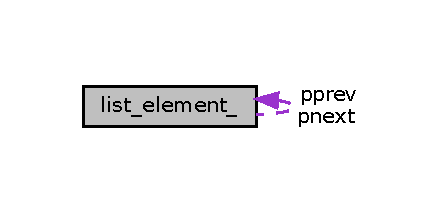
\includegraphics[width=200pt]{structlist__element____coll__graph}
\end{center}
\end{figure}
\subsection*{Public Attributes}
\begin{DoxyCompactItemize}
\item 
\hypertarget{structlist__element___a81cb2c54606be8120460bded0d919039}{}struct \hyperlink{structlist__element__}{list\+\_\+element\+\_\+} $\ast$ \hyperlink{structlist__element___a81cb2c54606be8120460bded0d919039}{pnext}\label{structlist__element___a81cb2c54606be8120460bded0d919039}

\begin{DoxyCompactList}\small\item\em pointer to the next element in the list \end{DoxyCompactList}\item 
\hypertarget{structlist__element___a0f6c573966c9d70d4a2ef19b73717515}{}struct \hyperlink{structlist__element__}{list\+\_\+element\+\_\+} $\ast$ \hyperlink{structlist__element___a0f6c573966c9d70d4a2ef19b73717515}{pprev}\label{structlist__element___a0f6c573966c9d70d4a2ef19b73717515}

\begin{DoxyCompactList}\small\item\em pointer to the previous element in the list \end{DoxyCompactList}\end{DoxyCompactItemize}


\subsection{Detailed Description}
structure defines base type for the lists 

The documentation for this struct was generated from the following file\+:\begin{DoxyCompactItemize}
\item 
src/lib/tiny\+\_\+list.\+h\end{DoxyCompactItemize}

\hypertarget{classTiny_1_1Packet}{}\section{Tiny\+:\+:Packet Class Reference}
\label{classTiny_1_1Packet}\index{Tiny\+::\+Packet@{Tiny\+::\+Packet}}


{\ttfamily \#include $<$Tiny\+Packet.\+h$>$}

\subsection*{Public Member Functions}
\begin{DoxyCompactItemize}
\item 
\hyperlink{classTiny_1_1Packet_aad47b3053945b29b1b46d76b31b72960}{Packet} (char $\ast$buf, size\+\_\+t \hyperlink{classTiny_1_1Packet_a47c24d500159d2268908b10c407d8d4d}{size})
\item 
void \hyperlink{classTiny_1_1Packet_a9bfdb9244515ef3dbf1056c1e37d0902}{clear} ()
\item 
void \hyperlink{classTiny_1_1Packet_a52c746f604ee6c0e4e78902b4cf710a9}{put} (uint8\+\_\+t byte)
\item 
void \hyperlink{classTiny_1_1Packet_a6e1e5236908290f28c3b9a0818242b5b}{put} (char chr)
\item 
void \hyperlink{classTiny_1_1Packet_a0055b5d1c437104e38bf66ece8ab84ba}{put} (uint16\+\_\+t \hyperlink{classTiny_1_1Packet_a3307ba504caba9c5eee8f1f32cf1a749}{data})
\item 
void \hyperlink{classTiny_1_1Packet_aed30fc087142669b37ec99d9d6572e57}{put} (uint32\+\_\+t \hyperlink{classTiny_1_1Packet_a3307ba504caba9c5eee8f1f32cf1a749}{data})
\item 
void \hyperlink{classTiny_1_1Packet_a464ddc51642812e604ac39f775762165}{put} (int16\+\_\+t \hyperlink{classTiny_1_1Packet_a3307ba504caba9c5eee8f1f32cf1a749}{data})
\item 
void \hyperlink{classTiny_1_1Packet_a6b5880ebffa02df3a380a270809433e1}{put} (const char $\ast$str)
\item 
void \hyperlink{classTiny_1_1Packet_a5741e3aec04c9100ce00a6b702417231}{put} (const \hyperlink{classTiny_1_1Packet}{Packet} \&pkt)
\item 
void \hyperlink{classTiny_1_1Packet_ae8764bf70fd6f09df2cb15c02ce2aa30}{put\+Uid} (uint16\+\_\+t uid)
\item 
uint8\+\_\+t \hyperlink{classTiny_1_1Packet_a152feac05d3e972f614c17c36bf30513}{get\+Byte} ()
\item 
char \hyperlink{classTiny_1_1Packet_a260645f9d055da878f149a13ecd58844}{get\+Char} ()
\item 
uint16\+\_\+t \hyperlink{classTiny_1_1Packet_a71765e73adfbc67138f75c2b8ea7d74c}{get\+Uint16} ()
\item 
int16\+\_\+t \hyperlink{classTiny_1_1Packet_a7dfed04418564f93dd4d2b4e9144a861}{get\+Int16} ()
\item 
uint32\+\_\+t \hyperlink{classTiny_1_1Packet_a5dd4b89cb7224b62d4f0328c8e40f38f}{get\+Uint32} ()
\item 
char $\ast$ \hyperlink{classTiny_1_1Packet_a8bc9a3b3f41be292f9c5ac566afeb04b}{get\+String} ()
\item 
uint16\+\_\+t \hyperlink{classTiny_1_1Packet_a65e342e15b9fa3e878393d268c4e69e4}{get\+Uid} () const
\item 
size\+\_\+t \hyperlink{classTiny_1_1Packet_a47c24d500159d2268908b10c407d8d4d}{size} () const
\item 
size\+\_\+t \hyperlink{classTiny_1_1Packet_a9985ff3b48f81628a7428b1197ca9f8f}{max\+Size} () const
\item 
char $\ast$ \hyperlink{classTiny_1_1Packet_a3307ba504caba9c5eee8f1f32cf1a749}{data} ()
\item 
uint8\+\_\+t \& \hyperlink{classTiny_1_1Packet_abfaef504eb88a4db88bca3b907770fa2}{operator\mbox{[}$\,$\mbox{]}} (size\+\_\+t idx)
\item 
\hyperlink{classTiny_1_1Packet}{Packet} \& \hyperlink{classTiny_1_1Packet_a2de2c7f2c3ea6baaab462dd7e4469ecb}{operator=} (char chr)
\end{DoxyCompactItemize}
\subsection*{Friends}
\begin{DoxyCompactItemize}
\item 
\mbox{\Hypertarget{classTiny_1_1Packet_a45bd055fddab40aaf0c60bfb9e21aa6f}\label{classTiny_1_1Packet_a45bd055fddab40aaf0c60bfb9e21aa6f}} 
class {\bfseries Proto}
\item 
\mbox{\Hypertarget{classTiny_1_1Packet_a7f90e063a34c3417ed1ea25e64608857}\label{classTiny_1_1Packet_a7f90e063a34c3417ed1ea25e64608857}} 
class {\bfseries Proto\+Hd}
\item 
\mbox{\Hypertarget{classTiny_1_1Packet_a1d317236f2a79fa559d5a9112e555882}\label{classTiny_1_1Packet_a1d317236f2a79fa559d5a9112e555882}} 
class {\bfseries Proto\+Light}
\end{DoxyCompactItemize}


\subsection{Detailed Description}
Describes packet entity and provides A\+PI methods to manipulate the packet. 

\subsection{Constructor \& Destructor Documentation}
\mbox{\Hypertarget{classTiny_1_1Packet_aad47b3053945b29b1b46d76b31b72960}\label{classTiny_1_1Packet_aad47b3053945b29b1b46d76b31b72960}} 
\index{Tiny\+::\+Packet@{Tiny\+::\+Packet}!Packet@{Packet}}
\index{Packet@{Packet}!Tiny\+::\+Packet@{Tiny\+::\+Packet}}
\subsubsection{\texorpdfstring{Packet()}{Packet()}}
{\footnotesize\ttfamily Tiny\+::\+Packet\+::\+Packet (\begin{DoxyParamCaption}\item[{char $\ast$}]{buf,  }\item[{size\+\_\+t}]{size }\end{DoxyParamCaption})\hspace{0.3cm}{\ttfamily [inline]}}

Creates packet object. 
\begin{DoxyParams}{Parameters}
{\em buf} & -\/ pointer to the buffer to store packet data \\
\hline
{\em size} & -\/ size of the buffer to hold packet data \\
\hline
\end{DoxyParams}
\begin{DoxyNote}{Note}
passed buffer must exist all lifecycle of the \hyperlink{classTiny_1_1Packet}{Packet} object. 
\end{DoxyNote}


\subsection{Member Function Documentation}
\mbox{\Hypertarget{classTiny_1_1Packet_a9bfdb9244515ef3dbf1056c1e37d0902}\label{classTiny_1_1Packet_a9bfdb9244515ef3dbf1056c1e37d0902}} 
\index{Tiny\+::\+Packet@{Tiny\+::\+Packet}!clear@{clear}}
\index{clear@{clear}!Tiny\+::\+Packet@{Tiny\+::\+Packet}}
\subsubsection{\texorpdfstring{clear()}{clear()}}
{\footnotesize\ttfamily void Tiny\+::\+Packet\+::clear (\begin{DoxyParamCaption}{ }\end{DoxyParamCaption})\hspace{0.3cm}{\ttfamily [inline]}}

Clears \hyperlink{classTiny_1_1Packet}{Packet} state. Buffer and its size are preserved. \mbox{\Hypertarget{classTiny_1_1Packet_a3307ba504caba9c5eee8f1f32cf1a749}\label{classTiny_1_1Packet_a3307ba504caba9c5eee8f1f32cf1a749}} 
\index{Tiny\+::\+Packet@{Tiny\+::\+Packet}!data@{data}}
\index{data@{data}!Tiny\+::\+Packet@{Tiny\+::\+Packet}}
\subsubsection{\texorpdfstring{data()}{data()}}
{\footnotesize\ttfamily char$\ast$ Tiny\+::\+Packet\+::data (\begin{DoxyParamCaption}{ }\end{DoxyParamCaption})\hspace{0.3cm}{\ttfamily [inline]}}

Returns size of payload data in the received packet. \begin{DoxyReturn}{Returns}
size of payload data. 
\end{DoxyReturn}
\mbox{\Hypertarget{classTiny_1_1Packet_a152feac05d3e972f614c17c36bf30513}\label{classTiny_1_1Packet_a152feac05d3e972f614c17c36bf30513}} 
\index{Tiny\+::\+Packet@{Tiny\+::\+Packet}!get\+Byte@{get\+Byte}}
\index{get\+Byte@{get\+Byte}!Tiny\+::\+Packet@{Tiny\+::\+Packet}}
\subsubsection{\texorpdfstring{get\+Byte()}{getByte()}}
{\footnotesize\ttfamily uint8\+\_\+t Tiny\+::\+Packet\+::get\+Byte (\begin{DoxyParamCaption}{ }\end{DoxyParamCaption})\hspace{0.3cm}{\ttfamily [inline]}}

Reads next byte from the packet. \begin{DoxyReturn}{Returns}
byte from the packet. 
\end{DoxyReturn}
\mbox{\Hypertarget{classTiny_1_1Packet_a260645f9d055da878f149a13ecd58844}\label{classTiny_1_1Packet_a260645f9d055da878f149a13ecd58844}} 
\index{Tiny\+::\+Packet@{Tiny\+::\+Packet}!get\+Char@{get\+Char}}
\index{get\+Char@{get\+Char}!Tiny\+::\+Packet@{Tiny\+::\+Packet}}
\subsubsection{\texorpdfstring{get\+Char()}{getChar()}}
{\footnotesize\ttfamily char Tiny\+::\+Packet\+::get\+Char (\begin{DoxyParamCaption}{ }\end{DoxyParamCaption})\hspace{0.3cm}{\ttfamily [inline]}}

Reads next character from the packet. \begin{DoxyReturn}{Returns}
character from the packet. 
\end{DoxyReturn}
\mbox{\Hypertarget{classTiny_1_1Packet_a7dfed04418564f93dd4d2b4e9144a861}\label{classTiny_1_1Packet_a7dfed04418564f93dd4d2b4e9144a861}} 
\index{Tiny\+::\+Packet@{Tiny\+::\+Packet}!get\+Int16@{get\+Int16}}
\index{get\+Int16@{get\+Int16}!Tiny\+::\+Packet@{Tiny\+::\+Packet}}
\subsubsection{\texorpdfstring{get\+Int16()}{getInt16()}}
{\footnotesize\ttfamily int16\+\_\+t Tiny\+::\+Packet\+::get\+Int16 (\begin{DoxyParamCaption}{ }\end{DoxyParamCaption})\hspace{0.3cm}{\ttfamily [inline]}}

Reads next signed 16-\/bit integer from the packet. \begin{DoxyReturn}{Returns}
signed 16-\/bit integer. 
\end{DoxyReturn}
\mbox{\Hypertarget{classTiny_1_1Packet_a8bc9a3b3f41be292f9c5ac566afeb04b}\label{classTiny_1_1Packet_a8bc9a3b3f41be292f9c5ac566afeb04b}} 
\index{Tiny\+::\+Packet@{Tiny\+::\+Packet}!get\+String@{get\+String}}
\index{get\+String@{get\+String}!Tiny\+::\+Packet@{Tiny\+::\+Packet}}
\subsubsection{\texorpdfstring{get\+String()}{getString()}}
{\footnotesize\ttfamily char$\ast$ Tiny\+::\+Packet\+::get\+String (\begin{DoxyParamCaption}{ }\end{DoxyParamCaption})\hspace{0.3cm}{\ttfamily [inline]}}

Reads zero-\/terminated string from the packet. \begin{DoxyReturn}{Returns}
zero-\/terminated string. 
\end{DoxyReturn}
\mbox{\Hypertarget{classTiny_1_1Packet_a65e342e15b9fa3e878393d268c4e69e4}\label{classTiny_1_1Packet_a65e342e15b9fa3e878393d268c4e69e4}} 
\index{Tiny\+::\+Packet@{Tiny\+::\+Packet}!get\+Uid@{get\+Uid}}
\index{get\+Uid@{get\+Uid}!Tiny\+::\+Packet@{Tiny\+::\+Packet}}
\subsubsection{\texorpdfstring{get\+Uid()}{getUid()}}
{\footnotesize\ttfamily uint16\+\_\+t Tiny\+::\+Packet\+::get\+Uid (\begin{DoxyParamCaption}{ }\end{DoxyParamCaption}) const\hspace{0.3cm}{\ttfamily [inline]}}

Returns 16-\/bit identificator of the packet. \begin{DoxyWarning}{Warning}
uid is valid only if uid functionality is enabled in the \hyperlink{classTiny_1_1Proto}{Proto} 
\end{DoxyWarning}
\begin{DoxySeeAlso}{See also}
\hyperlink{classTiny_1_1Proto_a9fdd64b8296e27f3205cd0d3ea685eac}{Proto\+::enable\+Uid} 

\hyperlink{classTiny_1_1Proto_aff9f3c59f58a8ca527ad0254ab806c5c}{Proto\+::disable\+Uid} 
\end{DoxySeeAlso}
\begin{DoxyReturn}{Returns}
16-\/bit uid. 
\end{DoxyReturn}
\mbox{\Hypertarget{classTiny_1_1Packet_a71765e73adfbc67138f75c2b8ea7d74c}\label{classTiny_1_1Packet_a71765e73adfbc67138f75c2b8ea7d74c}} 
\index{Tiny\+::\+Packet@{Tiny\+::\+Packet}!get\+Uint16@{get\+Uint16}}
\index{get\+Uint16@{get\+Uint16}!Tiny\+::\+Packet@{Tiny\+::\+Packet}}
\subsubsection{\texorpdfstring{get\+Uint16()}{getUint16()}}
{\footnotesize\ttfamily uint16\+\_\+t Tiny\+::\+Packet\+::get\+Uint16 (\begin{DoxyParamCaption}{ }\end{DoxyParamCaption})\hspace{0.3cm}{\ttfamily [inline]}}

Reads next unsigned 16-\/bit integer from the packet. \begin{DoxyReturn}{Returns}
unsigned 16-\/bit integer. 
\end{DoxyReturn}
\mbox{\Hypertarget{classTiny_1_1Packet_a5dd4b89cb7224b62d4f0328c8e40f38f}\label{classTiny_1_1Packet_a5dd4b89cb7224b62d4f0328c8e40f38f}} 
\index{Tiny\+::\+Packet@{Tiny\+::\+Packet}!get\+Uint32@{get\+Uint32}}
\index{get\+Uint32@{get\+Uint32}!Tiny\+::\+Packet@{Tiny\+::\+Packet}}
\subsubsection{\texorpdfstring{get\+Uint32()}{getUint32()}}
{\footnotesize\ttfamily uint32\+\_\+t Tiny\+::\+Packet\+::get\+Uint32 (\begin{DoxyParamCaption}{ }\end{DoxyParamCaption})\hspace{0.3cm}{\ttfamily [inline]}}

Reads next unsigned 32-\/bit integer from the packet. \begin{DoxyReturn}{Returns}
unsigned 32-\/bit integer. 
\end{DoxyReturn}
\mbox{\Hypertarget{classTiny_1_1Packet_a9985ff3b48f81628a7428b1197ca9f8f}\label{classTiny_1_1Packet_a9985ff3b48f81628a7428b1197ca9f8f}} 
\index{Tiny\+::\+Packet@{Tiny\+::\+Packet}!max\+Size@{max\+Size}}
\index{max\+Size@{max\+Size}!Tiny\+::\+Packet@{Tiny\+::\+Packet}}
\subsubsection{\texorpdfstring{max\+Size()}{maxSize()}}
{\footnotesize\ttfamily size\+\_\+t Tiny\+::\+Packet\+::max\+Size (\begin{DoxyParamCaption}{ }\end{DoxyParamCaption}) const\hspace{0.3cm}{\ttfamily [inline]}}

Returns maximum size of packet buffer. \begin{DoxyReturn}{Returns}
max size of packet buffer. 
\end{DoxyReturn}
\mbox{\Hypertarget{classTiny_1_1Packet_a2de2c7f2c3ea6baaab462dd7e4469ecb}\label{classTiny_1_1Packet_a2de2c7f2c3ea6baaab462dd7e4469ecb}} 
\index{Tiny\+::\+Packet@{Tiny\+::\+Packet}!operator=@{operator=}}
\index{operator=@{operator=}!Tiny\+::\+Packet@{Tiny\+::\+Packet}}
\subsubsection{\texorpdfstring{operator=()}{operator=()}}
{\footnotesize\ttfamily \hyperlink{classTiny_1_1Packet}{Packet}\& Tiny\+::\+Packet\+::operator= (\begin{DoxyParamCaption}\item[{char}]{chr }\end{DoxyParamCaption})\hspace{0.3cm}{\ttfamily [inline]}}

Assign operator = puts next char to the packet. Several assign operators put one by one several chars. \mbox{\Hypertarget{classTiny_1_1Packet_abfaef504eb88a4db88bca3b907770fa2}\label{classTiny_1_1Packet_abfaef504eb88a4db88bca3b907770fa2}} 
\index{Tiny\+::\+Packet@{Tiny\+::\+Packet}!operator\mbox{[}\mbox{]}@{operator[]}}
\index{operator\mbox{[}\mbox{]}@{operator[]}!Tiny\+::\+Packet@{Tiny\+::\+Packet}}
\subsubsection{\texorpdfstring{operator[]()}{operator[]()}}
{\footnotesize\ttfamily uint8\+\_\+t\& Tiny\+::\+Packet\+::operator\mbox{[}$\,$\mbox{]} (\begin{DoxyParamCaption}\item[{size\+\_\+t}]{idx }\end{DoxyParamCaption})\hspace{0.3cm}{\ttfamily [inline]}}

You may refer to \hyperlink{classTiny_1_1Packet}{Packet} payload data directly by using operator \mbox{[}\mbox{]} \mbox{\Hypertarget{classTiny_1_1Packet_a52c746f604ee6c0e4e78902b4cf710a9}\label{classTiny_1_1Packet_a52c746f604ee6c0e4e78902b4cf710a9}} 
\index{Tiny\+::\+Packet@{Tiny\+::\+Packet}!put@{put}}
\index{put@{put}!Tiny\+::\+Packet@{Tiny\+::\+Packet}}
\subsubsection{\texorpdfstring{put()}{put()}\hspace{0.1cm}{\footnotesize\ttfamily [1/7]}}
{\footnotesize\ttfamily void Tiny\+::\+Packet\+::put (\begin{DoxyParamCaption}\item[{uint8\+\_\+t}]{byte }\end{DoxyParamCaption})\hspace{0.3cm}{\ttfamily [inline]}}

Puts next byte to the packet. For example, after calling this method twice\+: put(5), put(10), -\/ the \hyperlink{classTiny_1_1Packet}{Packet} will contain 5,10. 
\begin{DoxyParams}{Parameters}
{\em byte} & -\/ data byte to put. \\
\hline
\end{DoxyParams}
\mbox{\Hypertarget{classTiny_1_1Packet_a6e1e5236908290f28c3b9a0818242b5b}\label{classTiny_1_1Packet_a6e1e5236908290f28c3b9a0818242b5b}} 
\index{Tiny\+::\+Packet@{Tiny\+::\+Packet}!put@{put}}
\index{put@{put}!Tiny\+::\+Packet@{Tiny\+::\+Packet}}
\subsubsection{\texorpdfstring{put()}{put()}\hspace{0.1cm}{\footnotesize\ttfamily [2/7]}}
{\footnotesize\ttfamily void Tiny\+::\+Packet\+::put (\begin{DoxyParamCaption}\item[{char}]{chr }\end{DoxyParamCaption})\hspace{0.3cm}{\ttfamily [inline]}}

Puts next char to the packet. For example, after calling this method twice\+: put(\textquotesingle{}a\textquotesingle{}), put(\textquotesingle{}c\textquotesingle{}), -\/ the \hyperlink{classTiny_1_1Packet}{Packet} will contain \textquotesingle{}ac\textquotesingle{}. 
\begin{DoxyParams}{Parameters}
{\em chr} & -\/ character to put. \\
\hline
\end{DoxyParams}
\mbox{\Hypertarget{classTiny_1_1Packet_a0055b5d1c437104e38bf66ece8ab84ba}\label{classTiny_1_1Packet_a0055b5d1c437104e38bf66ece8ab84ba}} 
\index{Tiny\+::\+Packet@{Tiny\+::\+Packet}!put@{put}}
\index{put@{put}!Tiny\+::\+Packet@{Tiny\+::\+Packet}}
\subsubsection{\texorpdfstring{put()}{put()}\hspace{0.1cm}{\footnotesize\ttfamily [3/7]}}
{\footnotesize\ttfamily void Tiny\+::\+Packet\+::put (\begin{DoxyParamCaption}\item[{uint16\+\_\+t}]{data }\end{DoxyParamCaption})\hspace{0.3cm}{\ttfamily [inline]}}

Puts next 16-\/bit unsigned integer to the packet. 
\begin{DoxyParams}{Parameters}
{\em data} & -\/ data to put. \\
\hline
\end{DoxyParams}
\mbox{\Hypertarget{classTiny_1_1Packet_aed30fc087142669b37ec99d9d6572e57}\label{classTiny_1_1Packet_aed30fc087142669b37ec99d9d6572e57}} 
\index{Tiny\+::\+Packet@{Tiny\+::\+Packet}!put@{put}}
\index{put@{put}!Tiny\+::\+Packet@{Tiny\+::\+Packet}}
\subsubsection{\texorpdfstring{put()}{put()}\hspace{0.1cm}{\footnotesize\ttfamily [4/7]}}
{\footnotesize\ttfamily void Tiny\+::\+Packet\+::put (\begin{DoxyParamCaption}\item[{uint32\+\_\+t}]{data }\end{DoxyParamCaption})\hspace{0.3cm}{\ttfamily [inline]}}

Puts next 32-\/bit unsigned integer to the packet. 
\begin{DoxyParams}{Parameters}
{\em data} & -\/ data to put. \\
\hline
\end{DoxyParams}
\mbox{\Hypertarget{classTiny_1_1Packet_a464ddc51642812e604ac39f775762165}\label{classTiny_1_1Packet_a464ddc51642812e604ac39f775762165}} 
\index{Tiny\+::\+Packet@{Tiny\+::\+Packet}!put@{put}}
\index{put@{put}!Tiny\+::\+Packet@{Tiny\+::\+Packet}}
\subsubsection{\texorpdfstring{put()}{put()}\hspace{0.1cm}{\footnotesize\ttfamily [5/7]}}
{\footnotesize\ttfamily void Tiny\+::\+Packet\+::put (\begin{DoxyParamCaption}\item[{int16\+\_\+t}]{data }\end{DoxyParamCaption})\hspace{0.3cm}{\ttfamily [inline]}}

Puts next 16-\/bit signed integer to the packet. 
\begin{DoxyParams}{Parameters}
{\em data} & -\/ data to put. \\
\hline
\end{DoxyParams}
\mbox{\Hypertarget{classTiny_1_1Packet_a6b5880ebffa02df3a380a270809433e1}\label{classTiny_1_1Packet_a6b5880ebffa02df3a380a270809433e1}} 
\index{Tiny\+::\+Packet@{Tiny\+::\+Packet}!put@{put}}
\index{put@{put}!Tiny\+::\+Packet@{Tiny\+::\+Packet}}
\subsubsection{\texorpdfstring{put()}{put()}\hspace{0.1cm}{\footnotesize\ttfamily [6/7]}}
{\footnotesize\ttfamily void Tiny\+::\+Packet\+::put (\begin{DoxyParamCaption}\item[{const char $\ast$}]{str }\end{DoxyParamCaption})\hspace{0.3cm}{\ttfamily [inline]}}

Puts next null-\/terminated string to the packet. 
\begin{DoxyParams}{Parameters}
{\em str} & -\/ string to put. \\
\hline
\end{DoxyParams}
\mbox{\Hypertarget{classTiny_1_1Packet_a5741e3aec04c9100ce00a6b702417231}\label{classTiny_1_1Packet_a5741e3aec04c9100ce00a6b702417231}} 
\index{Tiny\+::\+Packet@{Tiny\+::\+Packet}!put@{put}}
\index{put@{put}!Tiny\+::\+Packet@{Tiny\+::\+Packet}}
\subsubsection{\texorpdfstring{put()}{put()}\hspace{0.1cm}{\footnotesize\ttfamily [7/7]}}
{\footnotesize\ttfamily void Tiny\+::\+Packet\+::put (\begin{DoxyParamCaption}\item[{const \hyperlink{classTiny_1_1Packet}{Packet} \&}]{pkt }\end{DoxyParamCaption})\hspace{0.3cm}{\ttfamily [inline]}}

Adds data from packet to the new packet being built. 
\begin{DoxyParams}{Parameters}
{\em pkt} & -\/ reference to the \hyperlink{classTiny_1_1Packet}{Packet} to add. \\
\hline
\end{DoxyParams}
\mbox{\Hypertarget{classTiny_1_1Packet_ae8764bf70fd6f09df2cb15c02ce2aa30}\label{classTiny_1_1Packet_ae8764bf70fd6f09df2cb15c02ce2aa30}} 
\index{Tiny\+::\+Packet@{Tiny\+::\+Packet}!put\+Uid@{put\+Uid}}
\index{put\+Uid@{put\+Uid}!Tiny\+::\+Packet@{Tiny\+::\+Packet}}
\subsubsection{\texorpdfstring{put\+Uid()}{putUid()}}
{\footnotesize\ttfamily void Tiny\+::\+Packet\+::put\+Uid (\begin{DoxyParamCaption}\item[{uint16\+\_\+t}]{uid }\end{DoxyParamCaption})\hspace{0.3cm}{\ttfamily [inline]}}

Puts uid to the packet. \begin{DoxyWarning}{Warning}
uid is sent only if this functionality is enabled in the \hyperlink{classTiny_1_1Proto}{Proto}. 
\end{DoxyWarning}
\begin{DoxySeeAlso}{See also}
\hyperlink{classTiny_1_1Proto_a9fdd64b8296e27f3205cd0d3ea685eac}{Proto\+::enable\+Uid} 

\hyperlink{classTiny_1_1Proto_aff9f3c59f58a8ca527ad0254ab806c5c}{Proto\+::disable\+Uid} 
\end{DoxySeeAlso}

\begin{DoxyParams}{Parameters}
{\em uid} & -\/ 16-\/bit number to place to the packet. \\
\hline
\end{DoxyParams}
\mbox{\Hypertarget{classTiny_1_1Packet_a47c24d500159d2268908b10c407d8d4d}\label{classTiny_1_1Packet_a47c24d500159d2268908b10c407d8d4d}} 
\index{Tiny\+::\+Packet@{Tiny\+::\+Packet}!size@{size}}
\index{size@{size}!Tiny\+::\+Packet@{Tiny\+::\+Packet}}
\subsubsection{\texorpdfstring{size()}{size()}}
{\footnotesize\ttfamily size\+\_\+t Tiny\+::\+Packet\+::size (\begin{DoxyParamCaption}{ }\end{DoxyParamCaption}) const\hspace{0.3cm}{\ttfamily [inline]}}

Returns size of payload data in the received packet. \begin{DoxyReturn}{Returns}
size of payload data. 
\end{DoxyReturn}


The documentation for this class was generated from the following file\+:\begin{DoxyCompactItemize}
\item 
src/\hyperlink{TinyPacket_8h}{Tiny\+Packet.\+h}\end{DoxyCompactItemize}

\hypertarget{classTiny_1_1Proto}{}\section{Tiny\+:\+:Proto Class Reference}
\label{classTiny_1_1Proto}\index{Tiny\+::\+Proto@{Tiny\+::\+Proto}}


{\ttfamily \#include $<$Tiny\+Protocol.\+h$>$}

\subsection*{Public Member Functions}
\begin{DoxyCompactItemize}
\item 
void \hyperlink{classTiny_1_1Proto_a6f5f4ebec42dc6e679c25e79284d7705}{begin} (\hyperlink{tiny__proto__types_8h_aafd634660bba76cace57a8f9b01e044d}{write\+\_\+block\+\_\+cb\+\_\+t} writecb, \hyperlink{tiny__proto__types_8h_a15bec127d9ee63658563d62e92b5261b}{read\+\_\+block\+\_\+cb\+\_\+t} readcb)
\item 
void \hyperlink{classTiny_1_1Proto_a1dcad822337b6155148b1da9222fdd82}{begin\+To\+Serial} ()
\item 
void \hyperlink{classTiny_1_1Proto_a707f3112e0ca3651d4b0f3df6c19dd8c}{begin\+To\+Serial1} ()
\item 
void \hyperlink{classTiny_1_1Proto_a6d06cd3b1530e4986ce42a9987c522c4}{begin\+To\+Serial2} ()
\item 
void \hyperlink{classTiny_1_1Proto_aedbc025e1534105134e4a2499d32207c}{begin\+To\+Serial3} ()
\item 
void \hyperlink{classTiny_1_1Proto_ae9f52fa1c4f18981672ad7af12633d4e}{end} ()
\item 
int \hyperlink{classTiny_1_1Proto_a46fbc8b8681431b9b0a9a4b953a8dc33}{write} (char $\ast$buf, int size, uint8\+\_\+t flags=\hyperlink{group__FLAGS__GROUP_ga3a34267804581c5709d03f52d232b307}{T\+I\+N\+Y\+\_\+\+F\+L\+A\+G\+\_\+\+W\+A\+I\+T\+\_\+\+F\+O\+R\+E\+V\+ER})
\item 
int \hyperlink{classTiny_1_1Proto_acc00ac10509eaa11a83b0b88a2278b3e}{read} (char $\ast$buf, int size, uint8\+\_\+t flags=\hyperlink{group__FLAGS__GROUP_ga3a34267804581c5709d03f52d232b307}{T\+I\+N\+Y\+\_\+\+F\+L\+A\+G\+\_\+\+W\+A\+I\+T\+\_\+\+F\+O\+R\+E\+V\+ER})
\item 
int \hyperlink{classTiny_1_1Proto_ade93766700805a81be6a3317d846b276}{write} (\hyperlink{classTiny_1_1Packet}{Packet} \&pkt, uint8\+\_\+t flags=\hyperlink{group__FLAGS__GROUP_ga3a34267804581c5709d03f52d232b307}{T\+I\+N\+Y\+\_\+\+F\+L\+A\+G\+\_\+\+W\+A\+I\+T\+\_\+\+F\+O\+R\+E\+V\+ER})
\item 
int \hyperlink{classTiny_1_1Proto_aedef629f8b8968db7c8693bb45039651}{read} (\hyperlink{classTiny_1_1Packet}{Packet} \&pkt, uint8\+\_\+t flags=\hyperlink{group__FLAGS__GROUP_ga3a34267804581c5709d03f52d232b307}{T\+I\+N\+Y\+\_\+\+F\+L\+A\+G\+\_\+\+W\+A\+I\+T\+\_\+\+F\+O\+R\+E\+V\+ER})
\item 
void \hyperlink{classTiny_1_1Proto_a8992983d7ada115b0aa24db41594947c}{disable\+Crc} ()
\item 
bool \hyperlink{classTiny_1_1Proto_abb6cbae9a9944dc9ae0d756554f65a52}{enable\+Check\+Sum} ()
\item 
bool \hyperlink{classTiny_1_1Proto_a794afcac2ca15544247c34b059bc1289}{enable\+Crc16} ()
\item 
bool \hyperlink{classTiny_1_1Proto_a2ef1c80490d9343b896180ab8b8a6f77}{enable\+Crc32} ()
\item 
void \hyperlink{classTiny_1_1Proto_a9fdd64b8296e27f3205cd0d3ea685eac}{enable\+Uid} ()
\item 
void \hyperlink{classTiny_1_1Proto_aff9f3c59f58a8ca527ad0254ab806c5c}{disable\+Uid} ()
\end{DoxyCompactItemize}


\subsection{Detailed Description}
\hyperlink{classTiny_1_1Proto}{Proto} class incapsulates Protocol functionality. Remember that you may use always C-\/style A\+PI functions instead C++. Please refer to documentation. 

\subsection{Member Function Documentation}
\mbox{\Hypertarget{classTiny_1_1Proto_a6f5f4ebec42dc6e679c25e79284d7705}\label{classTiny_1_1Proto_a6f5f4ebec42dc6e679c25e79284d7705}} 
\index{Tiny\+::\+Proto@{Tiny\+::\+Proto}!begin@{begin}}
\index{begin@{begin}!Tiny\+::\+Proto@{Tiny\+::\+Proto}}
\subsubsection{\texorpdfstring{begin()}{begin()}}
{\footnotesize\ttfamily void Tiny\+::\+Proto\+::begin (\begin{DoxyParamCaption}\item[{\hyperlink{tiny__proto__types_8h_aafd634660bba76cace57a8f9b01e044d}{write\+\_\+block\+\_\+cb\+\_\+t}}]{writecb,  }\item[{\hyperlink{tiny__proto__types_8h_a15bec127d9ee63658563d62e92b5261b}{read\+\_\+block\+\_\+cb\+\_\+t}}]{readcb }\end{DoxyParamCaption})}

Initializes protocol internal variables. If you need to switch communication with other destination point, you can call this method one again after calling \hyperlink{classTiny_1_1Proto_ae9f52fa1c4f18981672ad7af12633d4e}{end()}. 
\begin{DoxyParams}{Parameters}
{\em writecb} & -\/ write function to some physical channel \\
\hline
{\em readcb} & -\/ read function from some physical channel \\
\hline
\end{DoxyParams}
\begin{DoxyReturn}{Returns}
None 
\end{DoxyReturn}
\mbox{\Hypertarget{classTiny_1_1Proto_a1dcad822337b6155148b1da9222fdd82}\label{classTiny_1_1Proto_a1dcad822337b6155148b1da9222fdd82}} 
\index{Tiny\+::\+Proto@{Tiny\+::\+Proto}!begin\+To\+Serial@{begin\+To\+Serial}}
\index{begin\+To\+Serial@{begin\+To\+Serial}!Tiny\+::\+Proto@{Tiny\+::\+Proto}}
\subsubsection{\texorpdfstring{begin\+To\+Serial()}{beginToSerial()}}
{\footnotesize\ttfamily void Tiny\+::\+Proto\+::begin\+To\+Serial (\begin{DoxyParamCaption}{ }\end{DoxyParamCaption})\hspace{0.3cm}{\ttfamily [inline]}}

Initializes protocol internal variables and redirects communication through Arduino Serial connection (Serial). \begin{DoxyReturn}{Returns}
None 
\end{DoxyReturn}
\mbox{\Hypertarget{classTiny_1_1Proto_a707f3112e0ca3651d4b0f3df6c19dd8c}\label{classTiny_1_1Proto_a707f3112e0ca3651d4b0f3df6c19dd8c}} 
\index{Tiny\+::\+Proto@{Tiny\+::\+Proto}!begin\+To\+Serial1@{begin\+To\+Serial1}}
\index{begin\+To\+Serial1@{begin\+To\+Serial1}!Tiny\+::\+Proto@{Tiny\+::\+Proto}}
\subsubsection{\texorpdfstring{begin\+To\+Serial1()}{beginToSerial1()}}
{\footnotesize\ttfamily void Tiny\+::\+Proto\+::begin\+To\+Serial1 (\begin{DoxyParamCaption}{ }\end{DoxyParamCaption})\hspace{0.3cm}{\ttfamily [inline]}}

Initializes protocol internal variables and redirects communication through Arduino Serial1 connection (Serial1). \begin{DoxyReturn}{Returns}
None 
\end{DoxyReturn}
\mbox{\Hypertarget{classTiny_1_1Proto_a6d06cd3b1530e4986ce42a9987c522c4}\label{classTiny_1_1Proto_a6d06cd3b1530e4986ce42a9987c522c4}} 
\index{Tiny\+::\+Proto@{Tiny\+::\+Proto}!begin\+To\+Serial2@{begin\+To\+Serial2}}
\index{begin\+To\+Serial2@{begin\+To\+Serial2}!Tiny\+::\+Proto@{Tiny\+::\+Proto}}
\subsubsection{\texorpdfstring{begin\+To\+Serial2()}{beginToSerial2()}}
{\footnotesize\ttfamily void Tiny\+::\+Proto\+::begin\+To\+Serial2 (\begin{DoxyParamCaption}{ }\end{DoxyParamCaption})\hspace{0.3cm}{\ttfamily [inline]}}

Initializes protocol internal variables and redirects communication through Arduino Serial2 connection (Serial2). \begin{DoxyReturn}{Returns}
None 
\end{DoxyReturn}
\mbox{\Hypertarget{classTiny_1_1Proto_aedbc025e1534105134e4a2499d32207c}\label{classTiny_1_1Proto_aedbc025e1534105134e4a2499d32207c}} 
\index{Tiny\+::\+Proto@{Tiny\+::\+Proto}!begin\+To\+Serial3@{begin\+To\+Serial3}}
\index{begin\+To\+Serial3@{begin\+To\+Serial3}!Tiny\+::\+Proto@{Tiny\+::\+Proto}}
\subsubsection{\texorpdfstring{begin\+To\+Serial3()}{beginToSerial3()}}
{\footnotesize\ttfamily void Tiny\+::\+Proto\+::begin\+To\+Serial3 (\begin{DoxyParamCaption}{ }\end{DoxyParamCaption})\hspace{0.3cm}{\ttfamily [inline]}}

Initializes protocol internal variables and redirects communication through Arduino Serial3 connection (Serial3). \begin{DoxyReturn}{Returns}
None 
\end{DoxyReturn}
\mbox{\Hypertarget{classTiny_1_1Proto_a8992983d7ada115b0aa24db41594947c}\label{classTiny_1_1Proto_a8992983d7ada115b0aa24db41594947c}} 
\index{Tiny\+::\+Proto@{Tiny\+::\+Proto}!disable\+Crc@{disable\+Crc}}
\index{disable\+Crc@{disable\+Crc}!Tiny\+::\+Proto@{Tiny\+::\+Proto}}
\subsubsection{\texorpdfstring{disable\+Crc()}{disableCrc()}}
{\footnotesize\ttfamily void Tiny\+::\+Proto\+::disable\+Crc (\begin{DoxyParamCaption}{ }\end{DoxyParamCaption})}

Disable C\+RC field in the protocol. If C\+RC field is O\+FF, then the frame looks like this\+: 0x7E databytes 0x7E. \mbox{\Hypertarget{classTiny_1_1Proto_aff9f3c59f58a8ca527ad0254ab806c5c}\label{classTiny_1_1Proto_aff9f3c59f58a8ca527ad0254ab806c5c}} 
\index{Tiny\+::\+Proto@{Tiny\+::\+Proto}!disable\+Uid@{disable\+Uid}}
\index{disable\+Uid@{disable\+Uid}!Tiny\+::\+Proto@{Tiny\+::\+Proto}}
\subsubsection{\texorpdfstring{disable\+Uid()}{disableUid()}}
{\footnotesize\ttfamily void Tiny\+::\+Proto\+::disable\+Uid (\begin{DoxyParamCaption}{ }\end{DoxyParamCaption})\hspace{0.3cm}{\ttfamily [inline]}}

Disables Uid field in the protocol. If enabled this 16-\/bit field with packet identifier is added before each payload data. Frame with uid\+: 0x7E 16-\/bituid payload 0x7E Frame without uid\+: 0x7E payload 0x7E \mbox{\Hypertarget{classTiny_1_1Proto_abb6cbae9a9944dc9ae0d756554f65a52}\label{classTiny_1_1Proto_abb6cbae9a9944dc9ae0d756554f65a52}} 
\index{Tiny\+::\+Proto@{Tiny\+::\+Proto}!enable\+Check\+Sum@{enable\+Check\+Sum}}
\index{enable\+Check\+Sum@{enable\+Check\+Sum}!Tiny\+::\+Proto@{Tiny\+::\+Proto}}
\subsubsection{\texorpdfstring{enable\+Check\+Sum()}{enableCheckSum()}}
{\footnotesize\ttfamily bool Tiny\+::\+Proto\+::enable\+Check\+Sum (\begin{DoxyParamCaption}{ }\end{DoxyParamCaption})}

Enables C\+RC 8-\/bit field in the protocol. This field contains sum of all data bytes in the packet. 8-\/bit field is supported by Nano version of Tiny library. \begin{DoxyReturn}{Returns}
true if successful false in case of error. 
\end{DoxyReturn}
\mbox{\Hypertarget{classTiny_1_1Proto_a794afcac2ca15544247c34b059bc1289}\label{classTiny_1_1Proto_a794afcac2ca15544247c34b059bc1289}} 
\index{Tiny\+::\+Proto@{Tiny\+::\+Proto}!enable\+Crc16@{enable\+Crc16}}
\index{enable\+Crc16@{enable\+Crc16}!Tiny\+::\+Proto@{Tiny\+::\+Proto}}
\subsubsection{\texorpdfstring{enable\+Crc16()}{enableCrc16()}}
{\footnotesize\ttfamily bool Tiny\+::\+Proto\+::enable\+Crc16 (\begin{DoxyParamCaption}{ }\end{DoxyParamCaption})}

Enables C\+RC 16-\/bit field in the protocol. This field contains F\+CS 16-\/bit C\+C\+I\+TT like defined in R\+FC 1662. 16-\/bit field is not supported by Nano version of Tiny library. \begin{DoxyReturn}{Returns}
true if successful false in case of error. 
\end{DoxyReturn}
\mbox{\Hypertarget{classTiny_1_1Proto_a2ef1c80490d9343b896180ab8b8a6f77}\label{classTiny_1_1Proto_a2ef1c80490d9343b896180ab8b8a6f77}} 
\index{Tiny\+::\+Proto@{Tiny\+::\+Proto}!enable\+Crc32@{enable\+Crc32}}
\index{enable\+Crc32@{enable\+Crc32}!Tiny\+::\+Proto@{Tiny\+::\+Proto}}
\subsubsection{\texorpdfstring{enable\+Crc32()}{enableCrc32()}}
{\footnotesize\ttfamily bool Tiny\+::\+Proto\+::enable\+Crc32 (\begin{DoxyParamCaption}{ }\end{DoxyParamCaption})}

Enables C\+RC 32-\/bit field in the protocol. This field contains F\+CS 32-\/bit C\+C\+I\+TT like defined in R\+FC 1662. 32-\/bit field is not supported by Nano version of Tiny library. \begin{DoxyReturn}{Returns}
true if successful false in case of error. 
\end{DoxyReturn}
\mbox{\Hypertarget{classTiny_1_1Proto_a9fdd64b8296e27f3205cd0d3ea685eac}\label{classTiny_1_1Proto_a9fdd64b8296e27f3205cd0d3ea685eac}} 
\index{Tiny\+::\+Proto@{Tiny\+::\+Proto}!enable\+Uid@{enable\+Uid}}
\index{enable\+Uid@{enable\+Uid}!Tiny\+::\+Proto@{Tiny\+::\+Proto}}
\subsubsection{\texorpdfstring{enable\+Uid()}{enableUid()}}
{\footnotesize\ttfamily void Tiny\+::\+Proto\+::enable\+Uid (\begin{DoxyParamCaption}{ }\end{DoxyParamCaption})\hspace{0.3cm}{\ttfamily [inline]}}

Enables Uid field in the protocol. If enabled this 16-\/bit field with packet identifier is added before each payload data. Frame with uid\+: 0x7E 16-\/bituid payload 0x7E Frame without uid\+: 0x7E payload 0x7E \mbox{\Hypertarget{classTiny_1_1Proto_ae9f52fa1c4f18981672ad7af12633d4e}\label{classTiny_1_1Proto_ae9f52fa1c4f18981672ad7af12633d4e}} 
\index{Tiny\+::\+Proto@{Tiny\+::\+Proto}!end@{end}}
\index{end@{end}!Tiny\+::\+Proto@{Tiny\+::\+Proto}}
\subsubsection{\texorpdfstring{end()}{end()}}
{\footnotesize\ttfamily void Tiny\+::\+Proto\+::end (\begin{DoxyParamCaption}{ }\end{DoxyParamCaption})}

Resets protocol state. \mbox{\Hypertarget{classTiny_1_1Proto_acc00ac10509eaa11a83b0b88a2278b3e}\label{classTiny_1_1Proto_acc00ac10509eaa11a83b0b88a2278b3e}} 
\index{Tiny\+::\+Proto@{Tiny\+::\+Proto}!read@{read}}
\index{read@{read}!Tiny\+::\+Proto@{Tiny\+::\+Proto}}
\subsubsection{\texorpdfstring{read()}{read()}\hspace{0.1cm}{\footnotesize\ttfamily [1/2]}}
{\footnotesize\ttfamily int Tiny\+::\+Proto\+::read (\begin{DoxyParamCaption}\item[{char $\ast$}]{buf,  }\item[{int}]{size,  }\item[{uint8\+\_\+t}]{flags = {\ttfamily \hyperlink{group__FLAGS__GROUP_ga3a34267804581c5709d03f52d232b307}{T\+I\+N\+Y\+\_\+\+F\+L\+A\+G\+\_\+\+W\+A\+I\+T\+\_\+\+F\+O\+R\+E\+V\+ER}} }\end{DoxyParamCaption})}

Reads data block from communication channel. 
\begin{DoxyParams}{Parameters}
{\em buf} & -\/ buffer to place data read from communication channel \\
\hline
{\em size} & -\/ maximum size of the buffer in bytes. \\
\hline
{\em flags} & -\/ \hyperlink{group__FLAGS__GROUP}{Flags for Tiny A\+PI functions} \\
\hline
\end{DoxyParams}
\begin{DoxyReturn}{Returns}
negative value in case of error zero if nothing is read positive -\/ number of bytes read from the channel 
\end{DoxyReturn}
\mbox{\Hypertarget{classTiny_1_1Proto_aedef629f8b8968db7c8693bb45039651}\label{classTiny_1_1Proto_aedef629f8b8968db7c8693bb45039651}} 
\index{Tiny\+::\+Proto@{Tiny\+::\+Proto}!read@{read}}
\index{read@{read}!Tiny\+::\+Proto@{Tiny\+::\+Proto}}
\subsubsection{\texorpdfstring{read()}{read()}\hspace{0.1cm}{\footnotesize\ttfamily [2/2]}}
{\footnotesize\ttfamily int Tiny\+::\+Proto\+::read (\begin{DoxyParamCaption}\item[{\hyperlink{classTiny_1_1Packet}{Packet} \&}]{pkt,  }\item[{uint8\+\_\+t}]{flags = {\ttfamily \hyperlink{group__FLAGS__GROUP_ga3a34267804581c5709d03f52d232b307}{T\+I\+N\+Y\+\_\+\+F\+L\+A\+G\+\_\+\+W\+A\+I\+T\+\_\+\+F\+O\+R\+E\+V\+ER}} }\end{DoxyParamCaption})}

Reads packet from communication channel. 
\begin{DoxyParams}{Parameters}
{\em pkt} & \hyperlink{classTiny_1_1Packet}{Packet} object to put data to \\
\hline
{\em flags} & \hyperlink{group__FLAGS__GROUP}{Flags for Tiny A\+PI functions} \\
\hline
\end{DoxyParams}
\begin{DoxySeeAlso}{See also}
\hyperlink{classTiny_1_1Packet}{Packet} 
\end{DoxySeeAlso}
\begin{DoxyReturn}{Returns}
negative value in case of error zero if nothing is read positive -\/ \hyperlink{classTiny_1_1Packet}{Packet} is successfully received 
\end{DoxyReturn}
\mbox{\Hypertarget{classTiny_1_1Proto_a46fbc8b8681431b9b0a9a4b953a8dc33}\label{classTiny_1_1Proto_a46fbc8b8681431b9b0a9a4b953a8dc33}} 
\index{Tiny\+::\+Proto@{Tiny\+::\+Proto}!write@{write}}
\index{write@{write}!Tiny\+::\+Proto@{Tiny\+::\+Proto}}
\subsubsection{\texorpdfstring{write()}{write()}\hspace{0.1cm}{\footnotesize\ttfamily [1/2]}}
{\footnotesize\ttfamily int Tiny\+::\+Proto\+::write (\begin{DoxyParamCaption}\item[{char $\ast$}]{buf,  }\item[{int}]{size,  }\item[{uint8\+\_\+t}]{flags = {\ttfamily \hyperlink{group__FLAGS__GROUP_ga3a34267804581c5709d03f52d232b307}{T\+I\+N\+Y\+\_\+\+F\+L\+A\+G\+\_\+\+W\+A\+I\+T\+\_\+\+F\+O\+R\+E\+V\+ER}} }\end{DoxyParamCaption})}

Sends data block over communication channel. 
\begin{DoxyParams}{Parameters}
{\em buf} & -\/ data to send \\
\hline
{\em size} & -\/ length of the data in bytes \\
\hline
{\em flags} & -\/ flags. \hyperlink{group__FLAGS__GROUP}{Flags for Tiny A\+PI functions} \\
\hline
\end{DoxyParams}
\begin{DoxyReturn}{Returns}
negative value in case of error zero if nothing is sent positive -\/ should be equal to size parameter 
\end{DoxyReturn}
\mbox{\Hypertarget{classTiny_1_1Proto_ade93766700805a81be6a3317d846b276}\label{classTiny_1_1Proto_ade93766700805a81be6a3317d846b276}} 
\index{Tiny\+::\+Proto@{Tiny\+::\+Proto}!write@{write}}
\index{write@{write}!Tiny\+::\+Proto@{Tiny\+::\+Proto}}
\subsubsection{\texorpdfstring{write()}{write()}\hspace{0.1cm}{\footnotesize\ttfamily [2/2]}}
{\footnotesize\ttfamily int Tiny\+::\+Proto\+::write (\begin{DoxyParamCaption}\item[{\hyperlink{classTiny_1_1Packet}{Packet} \&}]{pkt,  }\item[{uint8\+\_\+t}]{flags = {\ttfamily \hyperlink{group__FLAGS__GROUP_ga3a34267804581c5709d03f52d232b307}{T\+I\+N\+Y\+\_\+\+F\+L\+A\+G\+\_\+\+W\+A\+I\+T\+\_\+\+F\+O\+R\+E\+V\+ER}} }\end{DoxyParamCaption})}

Sends packet over communication channel. 
\begin{DoxyParams}{Parameters}
{\em pkt} & -\/ \hyperlink{classTiny_1_1Packet}{Packet} to send \\
\hline
{\em flags} & -\/ \hyperlink{group__FLAGS__GROUP}{Flags for Tiny A\+PI functions} \\
\hline
\end{DoxyParams}
\begin{DoxySeeAlso}{See also}
\hyperlink{classTiny_1_1Packet}{Packet} 
\end{DoxySeeAlso}
\begin{DoxyReturn}{Returns}
negative value in case of error zero if nothing is sent positive -\/ \hyperlink{classTiny_1_1Packet}{Packet} is successfully sent 
\end{DoxyReturn}


The documentation for this class was generated from the following file\+:\begin{DoxyCompactItemize}
\item 
src/\hyperlink{TinyProtocol_8h}{Tiny\+Protocol.\+h}\end{DoxyCompactItemize}

\hypertarget{classTiny_1_1ProtoHd}{}\section{Tiny\+:\+:Proto\+Hd Class Reference}
\label{classTiny_1_1ProtoHd}\index{Tiny\+::\+Proto\+Hd@{Tiny\+::\+Proto\+Hd}}


{\ttfamily \#include $<$Tiny\+Protocol\+Hd.\+h$>$}

\subsection*{Public Member Functions}
\begin{DoxyCompactItemize}
\item 
\hyperlink{classTiny_1_1ProtoHd_a1a55191980c259f2c760997d9c07cb48}{Proto\+Hd} (void $\ast$buffer, int buffer\+Size, void($\ast$on\+Receive)(uint8\+\_\+t $\ast$buf, int len))
\item 
void \hyperlink{classTiny_1_1ProtoHd_a112ae02531837a852af7ca3c9a32a7eb}{begin} (\hyperlink{tiny__proto__types_8h_a7f69e669de5baa69a43ee5cb439a7496}{write\+\_\+block\+\_\+cb\+\_\+t} writecb, \hyperlink{tiny__proto__types_8h_ae3d867e030f59de94508902f2b84a7ec}{read\+\_\+block\+\_\+cb\+\_\+t} readcb)
\item 
void \hyperlink{classTiny_1_1ProtoHd_a0e88ac5b3c67ca67c566742c22180050}{begin\+To\+Serial} ()
\item 
void \hyperlink{classTiny_1_1ProtoHd_a1b2975217b0523c3de4b534644cfa501}{begin\+To\+Serial1} ()
\item 
void \hyperlink{classTiny_1_1ProtoHd_a450fc792e515ffd150072988bc632c9e}{begin\+To\+Serial2} ()
\item 
void \hyperlink{classTiny_1_1ProtoHd_acd6519f6652c279b3a3b98aabbaeed65}{begin\+To\+Serial3} ()
\item 
void \hyperlink{classTiny_1_1ProtoHd_ac87bf8264895b654025001a0e6014f3f}{end} ()
\item 
int \hyperlink{classTiny_1_1ProtoHd_af53c8817317d3a62535e68ca236a038f}{write} (char $\ast$buf, int size)
\item 
int \hyperlink{classTiny_1_1ProtoHd_abffb26e95006c4e09e79f27f6ec4cdfe}{write} (\hyperlink{classTiny_1_1Packet}{Packet} \&pkt)
\item 
int \hyperlink{classTiny_1_1ProtoHd_af07b1f5d0df3021e00a4b4f04af4150b}{run} ()
\item 
void \hyperlink{classTiny_1_1ProtoHd_ae90a0a40de0b71a015f7f7f940440fa0}{disable\+Crc} ()
\item 
bool \hyperlink{classTiny_1_1ProtoHd_ace4e6b993532b3eb47d025b8db94192d}{enable\+Check\+Sum} ()
\item 
bool \hyperlink{classTiny_1_1ProtoHd_a0887adedc93b7538dbaef3fc8e0b2819}{enable\+Crc16} ()
\item 
bool \hyperlink{classTiny_1_1ProtoHd_a4110a0112548d5e47d312d190930ad20}{enable\+Crc32} ()
\end{DoxyCompactItemize}


\subsection{Detailed Description}
\hyperlink{classTiny_1_1ProtoHd}{Proto\+Hd} class incapsulates Half Duplex Protocol functionality. Half Duplex version of the Protocol allows to send messages with confirmation. Remember that you may use always C-\/style A\+PI functions instead C++. Please refer to documentation. 

\subsection{Constructor \& Destructor Documentation}
\mbox{\Hypertarget{classTiny_1_1ProtoHd_a1a55191980c259f2c760997d9c07cb48}\label{classTiny_1_1ProtoHd_a1a55191980c259f2c760997d9c07cb48}} 
\index{Tiny\+::\+Proto\+Hd@{Tiny\+::\+Proto\+Hd}!Proto\+Hd@{Proto\+Hd}}
\index{Proto\+Hd@{Proto\+Hd}!Tiny\+::\+Proto\+Hd@{Tiny\+::\+Proto\+Hd}}
\subsubsection{\texorpdfstring{Proto\+Hd()}{ProtoHd()}}
{\footnotesize\ttfamily Tiny\+::\+Proto\+Hd\+::\+Proto\+Hd (\begin{DoxyParamCaption}\item[{void $\ast$}]{buffer,  }\item[{int}]{buffer\+Size,  }\item[{void($\ast$)(uint8\+\_\+t $\ast$buf, int len)}]{on\+Receive }\end{DoxyParamCaption})\hspace{0.3cm}{\ttfamily [inline]}}

Initializes \hyperlink{classTiny_1_1ProtoHd}{Proto\+Hd} object 
\begin{DoxyParams}{Parameters}
{\em buffer} & -\/ buffer to store the frames being received. \\
\hline
{\em buffer\+Size} & -\/ size of the buffer \\
\hline
{\em on\+Receive} & -\/ callback to call when the frame is received completely. \\
\hline
\end{DoxyParams}


\subsection{Member Function Documentation}
\mbox{\Hypertarget{classTiny_1_1ProtoHd_a112ae02531837a852af7ca3c9a32a7eb}\label{classTiny_1_1ProtoHd_a112ae02531837a852af7ca3c9a32a7eb}} 
\index{Tiny\+::\+Proto\+Hd@{Tiny\+::\+Proto\+Hd}!begin@{begin}}
\index{begin@{begin}!Tiny\+::\+Proto\+Hd@{Tiny\+::\+Proto\+Hd}}
\subsubsection{\texorpdfstring{begin()}{begin()}}
{\footnotesize\ttfamily void Tiny\+::\+Proto\+Hd\+::begin (\begin{DoxyParamCaption}\item[{\hyperlink{tiny__proto__types_8h_a7f69e669de5baa69a43ee5cb439a7496}{write\+\_\+block\+\_\+cb\+\_\+t}}]{writecb,  }\item[{\hyperlink{tiny__proto__types_8h_ae3d867e030f59de94508902f2b84a7ec}{read\+\_\+block\+\_\+cb\+\_\+t}}]{readcb }\end{DoxyParamCaption})}

Initializes protocol internal variables. If you need to switch communication with other destination point, you can call this method one again after calling \hyperlink{classTiny_1_1ProtoHd_ac87bf8264895b654025001a0e6014f3f}{end()}. 
\begin{DoxyParams}{Parameters}
{\em writecb} & -\/ write function to some physical channel \\
\hline
{\em readcb} & -\/ read function from some physical channel \\
\hline
\end{DoxyParams}
\begin{DoxyReturn}{Returns}
None 
\end{DoxyReturn}
\mbox{\Hypertarget{classTiny_1_1ProtoHd_a0e88ac5b3c67ca67c566742c22180050}\label{classTiny_1_1ProtoHd_a0e88ac5b3c67ca67c566742c22180050}} 
\index{Tiny\+::\+Proto\+Hd@{Tiny\+::\+Proto\+Hd}!begin\+To\+Serial@{begin\+To\+Serial}}
\index{begin\+To\+Serial@{begin\+To\+Serial}!Tiny\+::\+Proto\+Hd@{Tiny\+::\+Proto\+Hd}}
\subsubsection{\texorpdfstring{begin\+To\+Serial()}{beginToSerial()}}
{\footnotesize\ttfamily void Tiny\+::\+Proto\+Hd\+::begin\+To\+Serial (\begin{DoxyParamCaption}{ }\end{DoxyParamCaption})\hspace{0.3cm}{\ttfamily [inline]}}

Initializes protocol internal variables and redirects communication through Arduino Serial connection (Serial). \begin{DoxyReturn}{Returns}
None 
\end{DoxyReturn}
\mbox{\Hypertarget{classTiny_1_1ProtoHd_a1b2975217b0523c3de4b534644cfa501}\label{classTiny_1_1ProtoHd_a1b2975217b0523c3de4b534644cfa501}} 
\index{Tiny\+::\+Proto\+Hd@{Tiny\+::\+Proto\+Hd}!begin\+To\+Serial1@{begin\+To\+Serial1}}
\index{begin\+To\+Serial1@{begin\+To\+Serial1}!Tiny\+::\+Proto\+Hd@{Tiny\+::\+Proto\+Hd}}
\subsubsection{\texorpdfstring{begin\+To\+Serial1()}{beginToSerial1()}}
{\footnotesize\ttfamily void Tiny\+::\+Proto\+Hd\+::begin\+To\+Serial1 (\begin{DoxyParamCaption}{ }\end{DoxyParamCaption})\hspace{0.3cm}{\ttfamily [inline]}}

Initializes protocol internal variables and redirects communication through Arduino Serial1 connection (Serial1). \begin{DoxyReturn}{Returns}
None 
\end{DoxyReturn}
\mbox{\Hypertarget{classTiny_1_1ProtoHd_a450fc792e515ffd150072988bc632c9e}\label{classTiny_1_1ProtoHd_a450fc792e515ffd150072988bc632c9e}} 
\index{Tiny\+::\+Proto\+Hd@{Tiny\+::\+Proto\+Hd}!begin\+To\+Serial2@{begin\+To\+Serial2}}
\index{begin\+To\+Serial2@{begin\+To\+Serial2}!Tiny\+::\+Proto\+Hd@{Tiny\+::\+Proto\+Hd}}
\subsubsection{\texorpdfstring{begin\+To\+Serial2()}{beginToSerial2()}}
{\footnotesize\ttfamily void Tiny\+::\+Proto\+Hd\+::begin\+To\+Serial2 (\begin{DoxyParamCaption}{ }\end{DoxyParamCaption})\hspace{0.3cm}{\ttfamily [inline]}}

Initializes protocol internal variables and redirects communication through Arduino Serial2 connection (Serial2). \begin{DoxyReturn}{Returns}
None 
\end{DoxyReturn}
\mbox{\Hypertarget{classTiny_1_1ProtoHd_acd6519f6652c279b3a3b98aabbaeed65}\label{classTiny_1_1ProtoHd_acd6519f6652c279b3a3b98aabbaeed65}} 
\index{Tiny\+::\+Proto\+Hd@{Tiny\+::\+Proto\+Hd}!begin\+To\+Serial3@{begin\+To\+Serial3}}
\index{begin\+To\+Serial3@{begin\+To\+Serial3}!Tiny\+::\+Proto\+Hd@{Tiny\+::\+Proto\+Hd}}
\subsubsection{\texorpdfstring{begin\+To\+Serial3()}{beginToSerial3()}}
{\footnotesize\ttfamily void Tiny\+::\+Proto\+Hd\+::begin\+To\+Serial3 (\begin{DoxyParamCaption}{ }\end{DoxyParamCaption})\hspace{0.3cm}{\ttfamily [inline]}}

Initializes protocol internal variables and redirects communication through Arduino Serial3 connection (Serial3). \begin{DoxyReturn}{Returns}
None 
\end{DoxyReturn}
\mbox{\Hypertarget{classTiny_1_1ProtoHd_ae90a0a40de0b71a015f7f7f940440fa0}\label{classTiny_1_1ProtoHd_ae90a0a40de0b71a015f7f7f940440fa0}} 
\index{Tiny\+::\+Proto\+Hd@{Tiny\+::\+Proto\+Hd}!disable\+Crc@{disable\+Crc}}
\index{disable\+Crc@{disable\+Crc}!Tiny\+::\+Proto\+Hd@{Tiny\+::\+Proto\+Hd}}
\subsubsection{\texorpdfstring{disable\+Crc()}{disableCrc()}}
{\footnotesize\ttfamily void Tiny\+::\+Proto\+Hd\+::disable\+Crc (\begin{DoxyParamCaption}{ }\end{DoxyParamCaption})}

Disable C\+RC field in the protocol. If C\+RC field is O\+FF, then the frame looks like this\+: 0x7E databytes 0x7E. \mbox{\Hypertarget{classTiny_1_1ProtoHd_ace4e6b993532b3eb47d025b8db94192d}\label{classTiny_1_1ProtoHd_ace4e6b993532b3eb47d025b8db94192d}} 
\index{Tiny\+::\+Proto\+Hd@{Tiny\+::\+Proto\+Hd}!enable\+Check\+Sum@{enable\+Check\+Sum}}
\index{enable\+Check\+Sum@{enable\+Check\+Sum}!Tiny\+::\+Proto\+Hd@{Tiny\+::\+Proto\+Hd}}
\subsubsection{\texorpdfstring{enable\+Check\+Sum()}{enableCheckSum()}}
{\footnotesize\ttfamily bool Tiny\+::\+Proto\+Hd\+::enable\+Check\+Sum (\begin{DoxyParamCaption}{ }\end{DoxyParamCaption})}

Enables C\+RC 8-\/bit field in the protocol. This field contains sum of all data bytes in the packet. 8-\/bit field is supported by Nano version of Tiny library. \begin{DoxyReturn}{Returns}
true if successful false in case of error. 
\end{DoxyReturn}
\mbox{\Hypertarget{classTiny_1_1ProtoHd_a0887adedc93b7538dbaef3fc8e0b2819}\label{classTiny_1_1ProtoHd_a0887adedc93b7538dbaef3fc8e0b2819}} 
\index{Tiny\+::\+Proto\+Hd@{Tiny\+::\+Proto\+Hd}!enable\+Crc16@{enable\+Crc16}}
\index{enable\+Crc16@{enable\+Crc16}!Tiny\+::\+Proto\+Hd@{Tiny\+::\+Proto\+Hd}}
\subsubsection{\texorpdfstring{enable\+Crc16()}{enableCrc16()}}
{\footnotesize\ttfamily bool Tiny\+::\+Proto\+Hd\+::enable\+Crc16 (\begin{DoxyParamCaption}{ }\end{DoxyParamCaption})}

Enables C\+RC 16-\/bit field in the protocol. This field contains F\+CS 16-\/bit C\+C\+I\+TT like defined in R\+FC 1662. 16-\/bit field is not supported by Nano version of Tiny library. \begin{DoxyReturn}{Returns}
true if successful false in case of error. 
\end{DoxyReturn}
\mbox{\Hypertarget{classTiny_1_1ProtoHd_a4110a0112548d5e47d312d190930ad20}\label{classTiny_1_1ProtoHd_a4110a0112548d5e47d312d190930ad20}} 
\index{Tiny\+::\+Proto\+Hd@{Tiny\+::\+Proto\+Hd}!enable\+Crc32@{enable\+Crc32}}
\index{enable\+Crc32@{enable\+Crc32}!Tiny\+::\+Proto\+Hd@{Tiny\+::\+Proto\+Hd}}
\subsubsection{\texorpdfstring{enable\+Crc32()}{enableCrc32()}}
{\footnotesize\ttfamily bool Tiny\+::\+Proto\+Hd\+::enable\+Crc32 (\begin{DoxyParamCaption}{ }\end{DoxyParamCaption})}

Enables C\+RC 32-\/bit field in the protocol. This field contains F\+CS 32-\/bit C\+C\+I\+TT like defined in R\+FC 1662. 32-\/bit field is not supported by Nano version of Tiny library. \begin{DoxyReturn}{Returns}
true if successful false in case of error. 
\end{DoxyReturn}
\mbox{\Hypertarget{classTiny_1_1ProtoHd_ac87bf8264895b654025001a0e6014f3f}\label{classTiny_1_1ProtoHd_ac87bf8264895b654025001a0e6014f3f}} 
\index{Tiny\+::\+Proto\+Hd@{Tiny\+::\+Proto\+Hd}!end@{end}}
\index{end@{end}!Tiny\+::\+Proto\+Hd@{Tiny\+::\+Proto\+Hd}}
\subsubsection{\texorpdfstring{end()}{end()}}
{\footnotesize\ttfamily void Tiny\+::\+Proto\+Hd\+::end (\begin{DoxyParamCaption}{ }\end{DoxyParamCaption})}

Resets protocol state. \mbox{\Hypertarget{classTiny_1_1ProtoHd_af07b1f5d0df3021e00a4b4f04af4150b}\label{classTiny_1_1ProtoHd_af07b1f5d0df3021e00a4b4f04af4150b}} 
\index{Tiny\+::\+Proto\+Hd@{Tiny\+::\+Proto\+Hd}!run@{run}}
\index{run@{run}!Tiny\+::\+Proto\+Hd@{Tiny\+::\+Proto\+Hd}}
\subsubsection{\texorpdfstring{run()}{run()}}
{\footnotesize\ttfamily int Tiny\+::\+Proto\+Hd\+::run (\begin{DoxyParamCaption}{ }\end{DoxyParamCaption})}

Checks communcation channel for incoming messages. \begin{DoxyReturn}{Returns}
negative value in case of error zero if nothing is read positive -\/ \hyperlink{classTiny_1_1Packet}{Packet} is successfully received 
\end{DoxyReturn}
\begin{DoxyRemark}{Remarks}
if \hyperlink{classTiny_1_1Packet}{Packet} is receive during run execution callback is called. 
\end{DoxyRemark}
\mbox{\Hypertarget{classTiny_1_1ProtoHd_af53c8817317d3a62535e68ca236a038f}\label{classTiny_1_1ProtoHd_af53c8817317d3a62535e68ca236a038f}} 
\index{Tiny\+::\+Proto\+Hd@{Tiny\+::\+Proto\+Hd}!write@{write}}
\index{write@{write}!Tiny\+::\+Proto\+Hd@{Tiny\+::\+Proto\+Hd}}
\subsubsection{\texorpdfstring{write()}{write()}\hspace{0.1cm}{\footnotesize\ttfamily [1/2]}}
{\footnotesize\ttfamily int Tiny\+::\+Proto\+Hd\+::write (\begin{DoxyParamCaption}\item[{char $\ast$}]{buf,  }\item[{int}]{size }\end{DoxyParamCaption})}

Sends data block over communication channel. 
\begin{DoxyParams}{Parameters}
{\em buf} & -\/ data to send \\
\hline
{\em size} & -\/ length of the data in bytes \\
\hline
\end{DoxyParams}
\begin{DoxyReturn}{Returns}
negative value in case of error zero if nothing is sent positive -\/ should be equal to size parameter 
\end{DoxyReturn}
\mbox{\Hypertarget{classTiny_1_1ProtoHd_abffb26e95006c4e09e79f27f6ec4cdfe}\label{classTiny_1_1ProtoHd_abffb26e95006c4e09e79f27f6ec4cdfe}} 
\index{Tiny\+::\+Proto\+Hd@{Tiny\+::\+Proto\+Hd}!write@{write}}
\index{write@{write}!Tiny\+::\+Proto\+Hd@{Tiny\+::\+Proto\+Hd}}
\subsubsection{\texorpdfstring{write()}{write()}\hspace{0.1cm}{\footnotesize\ttfamily [2/2]}}
{\footnotesize\ttfamily int Tiny\+::\+Proto\+Hd\+::write (\begin{DoxyParamCaption}\item[{\hyperlink{classTiny_1_1Packet}{Packet} \&}]{pkt }\end{DoxyParamCaption})}

Sends packet over communication channel. 
\begin{DoxyParams}{Parameters}
{\em pkt} & -\/ \hyperlink{classTiny_1_1Packet}{Packet} to send \\
\hline
\end{DoxyParams}
\begin{DoxySeeAlso}{See also}
\hyperlink{classTiny_1_1Packet}{Packet} 
\end{DoxySeeAlso}
\begin{DoxyReturn}{Returns}
negative value in case of error zero if nothing is sent positive -\/ \hyperlink{classTiny_1_1Packet}{Packet} is successfully sent 
\end{DoxyReturn}


The documentation for this class was generated from the following file\+:\begin{DoxyCompactItemize}
\item 
src/\hyperlink{TinyProtocolHd_8h}{Tiny\+Protocol\+Hd.\+h}\end{DoxyCompactItemize}

\hypertarget{classTiny_1_1ProtoLight}{}\section{Tiny\+:\+:Proto\+Light Class Reference}
\label{classTiny_1_1ProtoLight}\index{Tiny\+::\+Proto\+Light@{Tiny\+::\+Proto\+Light}}


{\ttfamily \#include $<$Tiny\+Light\+Protocol.\+h$>$}

\subsection*{Public Member Functions}
\begin{DoxyCompactItemize}
\item 
void \hyperlink{classTiny_1_1ProtoLight_ad27dfcef54a8316228469ef0a4267962}{begin} (write\+\_\+block\+\_\+cb\+\_\+t writecb, read\+\_\+block\+\_\+cb\+\_\+t readcb)
\item 
void \hyperlink{classTiny_1_1ProtoLight_a50bf63fe1891edda48980ca2893485d7}{begin\+To\+Serial} ()
\item 
void \hyperlink{classTiny_1_1ProtoLight_a948b2a0e37177b7434581adc64b36497}{end} ()
\item 
int \hyperlink{classTiny_1_1ProtoLight_a46a27ee9d0b55c88672c98abf04dbdce}{write} (char $\ast$buf, int size)
\item 
int \hyperlink{classTiny_1_1ProtoLight_acf18a8b73ee6c6394270c903ad7882b8}{read} (char $\ast$buf, int size)
\item 
int \hyperlink{classTiny_1_1ProtoLight_abf2966531f8ed7dba44079f00eefded2}{write} (\hyperlink{classTiny_1_1Packet}{Packet} \&pkt)
\item 
int \hyperlink{classTiny_1_1ProtoLight_a96c56b10b4eee28c09b291461c66fa54}{read} (\hyperlink{classTiny_1_1Packet}{Packet} \&pkt)
\end{DoxyCompactItemize}


\subsection{Detailed Description}
\hyperlink{classTiny_1_1ProtoLight}{Proto\+Light} class incapsulates Protocol functionality. Remember that you may use always C-\/style A\+P\+I functions instead C++. Please refer to documentation. 

\subsection{Member Function Documentation}
\hypertarget{classTiny_1_1ProtoLight_ad27dfcef54a8316228469ef0a4267962}{}\index{Tiny\+::\+Proto\+Light@{Tiny\+::\+Proto\+Light}!begin@{begin}}
\index{begin@{begin}!Tiny\+::\+Proto\+Light@{Tiny\+::\+Proto\+Light}}
\subsubsection[{begin}]{\setlength{\rightskip}{0pt plus 5cm}void Tiny\+::\+Proto\+Light\+::begin (
\begin{DoxyParamCaption}
\item[{write\+\_\+block\+\_\+cb\+\_\+t}]{writecb, }
\item[{read\+\_\+block\+\_\+cb\+\_\+t}]{readcb}
\end{DoxyParamCaption}
)}\label{classTiny_1_1ProtoLight_ad27dfcef54a8316228469ef0a4267962}
Initializes protocol internal variables. If you need to switch communication with other destination point, you can call this method one again after calling \hyperlink{classTiny_1_1ProtoLight_a948b2a0e37177b7434581adc64b36497}{end()}. 
\begin{DoxyParams}{Parameters}
{\em writecb} & -\/ write function to some physical channel \\
\hline
{\em readcb} & -\/ read function from some physical channel \\
\hline
\end{DoxyParams}
\begin{DoxyReturn}{Returns}
None 
\end{DoxyReturn}
\hypertarget{classTiny_1_1ProtoLight_a50bf63fe1891edda48980ca2893485d7}{}\index{Tiny\+::\+Proto\+Light@{Tiny\+::\+Proto\+Light}!begin\+To\+Serial@{begin\+To\+Serial}}
\index{begin\+To\+Serial@{begin\+To\+Serial}!Tiny\+::\+Proto\+Light@{Tiny\+::\+Proto\+Light}}
\subsubsection[{begin\+To\+Serial}]{\setlength{\rightskip}{0pt plus 5cm}void Tiny\+::\+Proto\+Light\+::begin\+To\+Serial (
\begin{DoxyParamCaption}
{}
\end{DoxyParamCaption}
)}\label{classTiny_1_1ProtoLight_a50bf63fe1891edda48980ca2893485d7}
Initializes protocol internal variables and redirects communication through Arduino Serial connection (Serial). \begin{DoxyReturn}{Returns}
None 
\end{DoxyReturn}
\hypertarget{classTiny_1_1ProtoLight_a948b2a0e37177b7434581adc64b36497}{}\index{Tiny\+::\+Proto\+Light@{Tiny\+::\+Proto\+Light}!end@{end}}
\index{end@{end}!Tiny\+::\+Proto\+Light@{Tiny\+::\+Proto\+Light}}
\subsubsection[{end}]{\setlength{\rightskip}{0pt plus 5cm}void Tiny\+::\+Proto\+Light\+::end (
\begin{DoxyParamCaption}
{}
\end{DoxyParamCaption}
)}\label{classTiny_1_1ProtoLight_a948b2a0e37177b7434581adc64b36497}
Resets protocol state. \hypertarget{classTiny_1_1ProtoLight_acf18a8b73ee6c6394270c903ad7882b8}{}\index{Tiny\+::\+Proto\+Light@{Tiny\+::\+Proto\+Light}!read@{read}}
\index{read@{read}!Tiny\+::\+Proto\+Light@{Tiny\+::\+Proto\+Light}}
\subsubsection[{read}]{\setlength{\rightskip}{0pt plus 5cm}int Tiny\+::\+Proto\+Light\+::read (
\begin{DoxyParamCaption}
\item[{char $\ast$}]{buf, }
\item[{int}]{size}
\end{DoxyParamCaption}
)}\label{classTiny_1_1ProtoLight_acf18a8b73ee6c6394270c903ad7882b8}
Reads data block from communication channel. 
\begin{DoxyParams}{Parameters}
{\em buf} & -\/ buffer to place data read from communication channel \\
\hline
{\em size} & -\/ maximum size of the buffer in bytes. \\
\hline
\end{DoxyParams}
\begin{DoxyReturn}{Returns}
negative value in case of error zero if nothing is read positive -\/ number of bytes read from the channel 
\end{DoxyReturn}
\hypertarget{classTiny_1_1ProtoLight_a96c56b10b4eee28c09b291461c66fa54}{}\index{Tiny\+::\+Proto\+Light@{Tiny\+::\+Proto\+Light}!read@{read}}
\index{read@{read}!Tiny\+::\+Proto\+Light@{Tiny\+::\+Proto\+Light}}
\subsubsection[{read}]{\setlength{\rightskip}{0pt plus 5cm}int Tiny\+::\+Proto\+Light\+::read (
\begin{DoxyParamCaption}
\item[{{\bf Packet} \&}]{pkt}
\end{DoxyParamCaption}
)}\label{classTiny_1_1ProtoLight_a96c56b10b4eee28c09b291461c66fa54}
Reads packet from communication channel. 
\begin{DoxyParams}{Parameters}
{\em pkt} & -\/ \hyperlink{classTiny_1_1Packet}{Packet} object to put data to \\
\hline
\end{DoxyParams}
\begin{DoxySeeAlso}{See also}
\hyperlink{classTiny_1_1Packet}{Packet} 
\end{DoxySeeAlso}
\begin{DoxyReturn}{Returns}
negative value in case of error zero if nothing is read positive -\/ \hyperlink{classTiny_1_1Packet}{Packet} is successfully received 
\end{DoxyReturn}
\hypertarget{classTiny_1_1ProtoLight_a46a27ee9d0b55c88672c98abf04dbdce}{}\index{Tiny\+::\+Proto\+Light@{Tiny\+::\+Proto\+Light}!write@{write}}
\index{write@{write}!Tiny\+::\+Proto\+Light@{Tiny\+::\+Proto\+Light}}
\subsubsection[{write}]{\setlength{\rightskip}{0pt plus 5cm}int Tiny\+::\+Proto\+Light\+::write (
\begin{DoxyParamCaption}
\item[{char $\ast$}]{buf, }
\item[{int}]{size}
\end{DoxyParamCaption}
)}\label{classTiny_1_1ProtoLight_a46a27ee9d0b55c88672c98abf04dbdce}
Sends data block over communication channel. 
\begin{DoxyParams}{Parameters}
{\em buf} & -\/ data to send \\
\hline
{\em size} & -\/ length of the data in bytes \\
\hline
\end{DoxyParams}
\begin{DoxyReturn}{Returns}
negative value in case of error zero if nothing is sent positive -\/ should be equal to size parameter 
\end{DoxyReturn}
\hypertarget{classTiny_1_1ProtoLight_abf2966531f8ed7dba44079f00eefded2}{}\index{Tiny\+::\+Proto\+Light@{Tiny\+::\+Proto\+Light}!write@{write}}
\index{write@{write}!Tiny\+::\+Proto\+Light@{Tiny\+::\+Proto\+Light}}
\subsubsection[{write}]{\setlength{\rightskip}{0pt plus 5cm}int Tiny\+::\+Proto\+Light\+::write (
\begin{DoxyParamCaption}
\item[{{\bf Packet} \&}]{pkt}
\end{DoxyParamCaption}
)}\label{classTiny_1_1ProtoLight_abf2966531f8ed7dba44079f00eefded2}
Sends packet over communication channel. 
\begin{DoxyParams}{Parameters}
{\em pkt} & -\/ \hyperlink{classTiny_1_1Packet}{Packet} to send \\
\hline
\end{DoxyParams}
\begin{DoxySeeAlso}{See also}
\hyperlink{classTiny_1_1Packet}{Packet} 
\end{DoxySeeAlso}
\begin{DoxyReturn}{Returns}
negative value in case of error zero if nothing is sent positive -\/ \hyperlink{classTiny_1_1Packet}{Packet} is successfully sent 
\end{DoxyReturn}


The documentation for this class was generated from the following file\+:\begin{DoxyCompactItemize}
\item 
src/arduino/src/\hyperlink{TinyLightProtocol_8h}{Tiny\+Light\+Protocol.\+h}\end{DoxyCompactItemize}

\hypertarget{structSTinyData}{}\section{S\+Tiny\+Data Struct Reference}
\label{structSTinyData}\index{S\+Tiny\+Data@{S\+Tiny\+Data}}


{\ttfamily \#include $<$tiny\+\_\+layer2.\+h$>$}



Collaboration diagram for S\+Tiny\+Data\+:\nopagebreak
\begin{figure}[H]
\begin{center}
\leavevmode
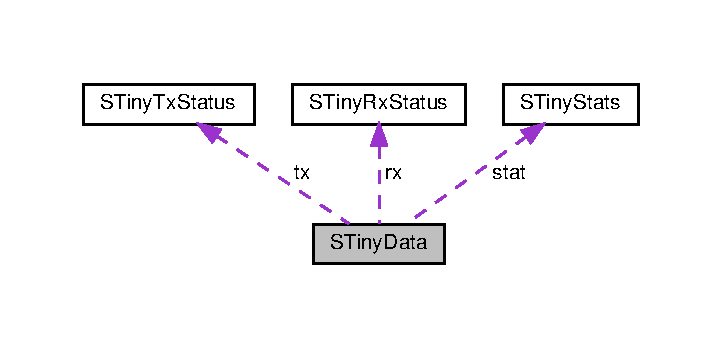
\includegraphics[width=347pt]{structSTinyData__coll__graph}
\end{center}
\end{figure}
\subsection*{Public Attributes}
\begin{DoxyCompactItemize}
\item 
\hypertarget{structSTinyData_a26c40b0b7e18776af99745624c460c5a}{}\hyperlink{tiny__layer2_8h_a7f69e669de5baa69a43ee5cb439a7496}{write\+\_\+block\+\_\+cb\+\_\+t} \hyperlink{structSTinyData_a26c40b0b7e18776af99745624c460c5a}{write\+\_\+func}\label{structSTinyData_a26c40b0b7e18776af99745624c460c5a}

\begin{DoxyCompactList}\small\item\em pointer to platform related write function \end{DoxyCompactList}\item 
\hypertarget{structSTinyData_a9714041284fd99230be0e7efbc8c60cf}{}\hyperlink{tiny__layer2_8h_ae3d867e030f59de94508902f2b84a7ec}{read\+\_\+block\+\_\+cb\+\_\+t} \hyperlink{structSTinyData_a9714041284fd99230be0e7efbc8c60cf}{read\+\_\+func}\label{structSTinyData_a9714041284fd99230be0e7efbc8c60cf}

\begin{DoxyCompactList}\small\item\em pointer to platform related read function \end{DoxyCompactList}\item 
\hypertarget{structSTinyData_a3ac48d44af9b2912dd980c7377a020be}{}void $\ast$ \hyperlink{structSTinyData_a3ac48d44af9b2912dd980c7377a020be}{pdata}\label{structSTinyData_a3ac48d44af9b2912dd980c7377a020be}

\begin{DoxyCompactList}\small\item\em pointer to application defined data, passed during protocol initialization -\/ absent in Arduino version \end{DoxyCompactList}\item 
\hyperlink{structSTinyRxStatus}{S\+Tiny\+Rx\+Status} \hyperlink{structSTinyData_aa3b43db99a1a6bf3d562f932d5a539db}{rx}
\item 
\hyperlink{structSTinyTxStatus}{S\+Tiny\+Tx\+Status} \hyperlink{structSTinyData_aa099adb35f3494332747eb18851fbb23}{tx}
\item 
\hypertarget{structSTinyData_a3cf4d6009cc472630e20a68d6fa50186}{}uint8\+\_\+t \hyperlink{structSTinyData_a3cf4d6009cc472630e20a68d6fa50186}{fcs\+\_\+bits}\label{structSTinyData_a3cf4d6009cc472630e20a68d6fa50186}

\begin{DoxyCompactList}\small\item\em The field contains number of bits to use for F\+C\+S and not available in T\+I\+N\+Y\+\_\+\+M\+I\+N\+I\+M\+A\+L configuration. \end{DoxyCompactList}\item 
\hyperlink{structSTinyStats}{S\+Tiny\+Stats} \hyperlink{structSTinyData_a16ba8c9e60d6aee3fcd4909f85561f3d}{stat}
\item 
\hyperlink{tiny__layer2_8h_ad6bf709565b8aecb9e6ecf196f219d54}{on\+\_\+frame\+\_\+cb\+\_\+t} \hyperlink{structSTinyData_a31ba50154472c11e0d063b0aeef95f4d}{read\+\_\+cb}
\begin{DoxyCompactList}\small\item\em pointer to callback function \end{DoxyCompactList}\item 
\hyperlink{tiny__layer2_8h_ad6bf709565b8aecb9e6ecf196f219d54}{on\+\_\+frame\+\_\+cb\+\_\+t} \hyperlink{structSTinyData_ada334c88e86bfd2c10191f65818c3fb3}{write\+\_\+cb}
\begin{DoxyCompactList}\small\item\em pointer to callback function to get data being sent \end{DoxyCompactList}\item 
\hypertarget{structSTinyData_aa004bdc7db38cbbef4df4a4d94ca6a4b}{}uint8\+\_\+t \hyperlink{structSTinyData_aa004bdc7db38cbbef4df4a4d94ca6a4b}{uid\+\_\+support}\label{structSTinyData_aa004bdc7db38cbbef4df4a4d94ca6a4b}

\begin{DoxyCompactList}\small\item\em flag indicates if uid support is enabled. It is important for \hyperlink{group__ADVANCED__API_gaaf9bf6423bd0b8388c3387225b805278}{tiny\+\_\+on\+\_\+rx\+\_\+byte()} \end{DoxyCompactList}\end{DoxyCompactItemize}


\subsection{Detailed Description}
This structure contains information about communication channel and its state. \begin{DoxyWarning}{Warning}
This is for internal use only, and should not be accessed directly from the application. 
\end{DoxyWarning}


\subsection{Member Data Documentation}
\hypertarget{structSTinyData_a31ba50154472c11e0d063b0aeef95f4d}{}\index{S\+Tiny\+Data@{S\+Tiny\+Data}!read\+\_\+cb@{read\+\_\+cb}}
\index{read\+\_\+cb@{read\+\_\+cb}!S\+Tiny\+Data@{S\+Tiny\+Data}}
\subsubsection[{read\+\_\+cb}]{\setlength{\rightskip}{0pt plus 5cm}{\bf on\+\_\+frame\+\_\+cb\+\_\+t} S\+Tiny\+Data\+::read\+\_\+cb}\label{structSTinyData_a31ba50154472c11e0d063b0aeef95f4d}


pointer to callback function 

This callback is called when it is not null and when new frame is successfully received. \hypertarget{structSTinyData_aa3b43db99a1a6bf3d562f932d5a539db}{}\index{S\+Tiny\+Data@{S\+Tiny\+Data}!rx@{rx}}
\index{rx@{rx}!S\+Tiny\+Data@{S\+Tiny\+Data}}
\subsubsection[{rx}]{\setlength{\rightskip}{0pt plus 5cm}{\bf S\+Tiny\+Rx\+Status} S\+Tiny\+Data\+::rx}\label{structSTinyData_aa3b43db99a1a6bf3d562f932d5a539db}
\begin{DoxySeeAlso}{See also}
\hyperlink{structSTinyRxStatus}{S\+Tiny\+Rx\+Status} 
\end{DoxySeeAlso}
\hypertarget{structSTinyData_a16ba8c9e60d6aee3fcd4909f85561f3d}{}\index{S\+Tiny\+Data@{S\+Tiny\+Data}!stat@{stat}}
\index{stat@{stat}!S\+Tiny\+Data@{S\+Tiny\+Data}}
\subsubsection[{stat}]{\setlength{\rightskip}{0pt plus 5cm}{\bf S\+Tiny\+Stats} S\+Tiny\+Data\+::stat}\label{structSTinyData_a16ba8c9e60d6aee3fcd4909f85561f3d}
\begin{DoxySeeAlso}{See also}
\hyperlink{structSTinyStats}{S\+Tiny\+Stats} 
\end{DoxySeeAlso}
\hypertarget{structSTinyData_aa099adb35f3494332747eb18851fbb23}{}\index{S\+Tiny\+Data@{S\+Tiny\+Data}!tx@{tx}}
\index{tx@{tx}!S\+Tiny\+Data@{S\+Tiny\+Data}}
\subsubsection[{tx}]{\setlength{\rightskip}{0pt plus 5cm}{\bf S\+Tiny\+Tx\+Status} S\+Tiny\+Data\+::tx}\label{structSTinyData_aa099adb35f3494332747eb18851fbb23}
\begin{DoxySeeAlso}{See also}
\hyperlink{structSTinyTxStatus}{S\+Tiny\+Tx\+Status} 
\end{DoxySeeAlso}
\hypertarget{structSTinyData_ada334c88e86bfd2c10191f65818c3fb3}{}\index{S\+Tiny\+Data@{S\+Tiny\+Data}!write\+\_\+cb@{write\+\_\+cb}}
\index{write\+\_\+cb@{write\+\_\+cb}!S\+Tiny\+Data@{S\+Tiny\+Data}}
\subsubsection[{write\+\_\+cb}]{\setlength{\rightskip}{0pt plus 5cm}{\bf on\+\_\+frame\+\_\+cb\+\_\+t} S\+Tiny\+Data\+::write\+\_\+cb}\label{structSTinyData_ada334c88e86bfd2c10191f65818c3fb3}


pointer to callback function to get data being sent 

This callback is called when it is not null and when new frame is successfully sent. 

The documentation for this struct was generated from the following file\+:\begin{DoxyCompactItemize}
\item 
inc/\hyperlink{tiny__layer2_8h}{tiny\+\_\+layer2.\+h}\end{DoxyCompactItemize}

\hypertarget{structSTinyHdData__}{}\section{S\+Tiny\+Hd\+Data\+\_\+ Struct Reference}
\label{structSTinyHdData__}\index{S\+Tiny\+Hd\+Data\+\_\+@{S\+Tiny\+Hd\+Data\+\_\+}}


{\ttfamily \#include $<$tiny\+\_\+hd.\+h$>$}



Collaboration diagram for S\+Tiny\+Hd\+Data\+\_\+\+:
\nopagebreak
\begin{figure}[H]
\begin{center}
\leavevmode
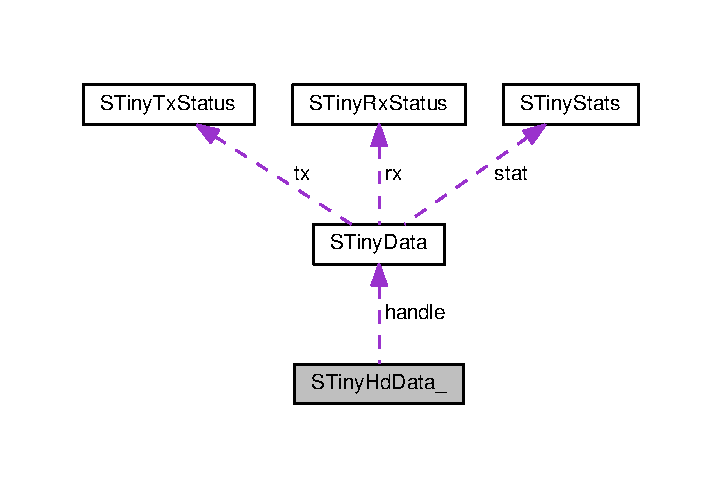
\includegraphics[width=263pt]{structSTinyHdData____coll__graph}
\end{center}
\end{figure}
\subsection*{Public Attributes}
\begin{DoxyCompactItemize}
\item 
\hypertarget{structSTinyHdData___a0df5a323cbbfd49fb138b14bca73f14c}{}\hyperlink{structSTinyData}{S\+Tiny\+Data} \hyperlink{structSTinyHdData___a0df5a323cbbfd49fb138b14bca73f14c}{handle}\label{structSTinyHdData___a0df5a323cbbfd49fb138b14bca73f14c}

\begin{DoxyCompactList}\small\item\em Original \hyperlink{structSTinyData}{S\+Tiny\+Data} structure. It is used to control lower level. \end{DoxyCompactList}\item 
\hypertarget{structSTinyHdData___abf8a0eb5006769a92adc186554a3a1c0}{}on\+\_\+frame\+\_\+cb\+\_\+t \hyperlink{structSTinyHdData___abf8a0eb5006769a92adc186554a3a1c0}{on\+\_\+frame\+\_\+cb}\label{structSTinyHdData___abf8a0eb5006769a92adc186554a3a1c0}

\begin{DoxyCompactList}\small\item\em Callback to process received frames. \end{DoxyCompactList}\item 
\hypertarget{structSTinyHdData___a69a6bb34b580bcfa5e13112cb7652d1d}{}void $\ast$ \hyperlink{structSTinyHdData___a69a6bb34b580bcfa5e13112cb7652d1d}{inbuf}\label{structSTinyHdData___a69a6bb34b580bcfa5e13112cb7652d1d}

\begin{DoxyCompactList}\small\item\em Buffer to store frames being received. \end{DoxyCompactList}\item 
\hypertarget{structSTinyHdData___adbad190a4b54eccd4da6f3c3305a54f1}{}uint16\+\_\+t \hyperlink{structSTinyHdData___adbad190a4b54eccd4da6f3c3305a54f1}{inbuf\+\_\+size}\label{structSTinyHdData___adbad190a4b54eccd4da6f3c3305a54f1}

\begin{DoxyCompactList}\small\item\em maximum size of Rx buffer \end{DoxyCompactList}\item 
\hypertarget{structSTinyHdData___a7ca4e5b23cf480d93317245010bcbe73}{}uint16\+\_\+t \hyperlink{structSTinyHdData___a7ca4e5b23cf480d93317245010bcbe73}{timeout}\label{structSTinyHdData___a7ca4e5b23cf480d93317245010bcbe73}

\begin{DoxyCompactList}\small\item\em Timeout for operations with acknowledge. \end{DoxyCompactList}\item 
\hypertarget{structSTinyHdData___a7084eac08b744ad0aa2624b854866825}{}uint16\+\_\+t \hyperlink{structSTinyHdData___a7084eac08b744ad0aa2624b854866825}{uid}\label{structSTinyHdData___a7084eac08b744ad0aa2624b854866825}

\begin{DoxyCompactList}\small\item\em field used to store temporary uid \end{DoxyCompactList}\item 
\hypertarget{structSTinyHdData___a37dca10adb0dd210f02365b7fa20a598}{}uint8\+\_\+t \hyperlink{structSTinyHdData___a37dca10adb0dd210f02365b7fa20a598}{multithread\+\_\+mode}\label{structSTinyHdData___a37dca10adb0dd210f02365b7fa20a598}

\begin{DoxyCompactList}\small\item\em only single thread mode is supporte now. Should be zero \end{DoxyCompactList}\end{DoxyCompactItemize}


\subsection{Detailed Description}
This structure contains service data, required for half-\/duplex functioning. 

The documentation for this struct was generated from the following file\+:\begin{DoxyCompactItemize}
\item 
inc/\hyperlink{tiny__hd_8h}{tiny\+\_\+hd.\+h}\end{DoxyCompactItemize}

\hypertarget{structSTinyHdInit__}{}\section{S\+Tiny\+Hd\+Init\+\_\+ Struct Reference}
\label{structSTinyHdInit__}\index{S\+Tiny\+Hd\+Init\+\_\+@{S\+Tiny\+Hd\+Init\+\_\+}}


{\ttfamily \#include $<$tiny\+\_\+hd.\+h$>$}

\subsection*{Public Attributes}
\begin{DoxyCompactItemize}
\item 
\mbox{\Hypertarget{structSTinyHdInit___a0bd05a4fc43236ff37d67aec4d2a0952}\label{structSTinyHdInit___a0bd05a4fc43236ff37d67aec4d2a0952}} 
\hyperlink{tiny__proto__types_8h_a7f69e669de5baa69a43ee5cb439a7496}{write\+\_\+block\+\_\+cb\+\_\+t} \hyperlink{structSTinyHdInit___a0bd05a4fc43236ff37d67aec4d2a0952}{write\+\_\+func}
\begin{DoxyCompactList}\small\item\em callback function to write bytes to the physical channel \end{DoxyCompactList}\item 
\mbox{\Hypertarget{structSTinyHdInit___a5de352b11ca7915737bc459cde7c566d}\label{structSTinyHdInit___a5de352b11ca7915737bc459cde7c566d}} 
\hyperlink{tiny__proto__types_8h_ae3d867e030f59de94508902f2b84a7ec}{read\+\_\+block\+\_\+cb\+\_\+t} \hyperlink{structSTinyHdInit___a5de352b11ca7915737bc459cde7c566d}{read\+\_\+func}
\begin{DoxyCompactList}\small\item\em callback function to read buytes from the physical channel \end{DoxyCompactList}\item 
\mbox{\Hypertarget{structSTinyHdInit___a7b6be4e09ea04eaa4372eadce4d51055}\label{structSTinyHdInit___a7b6be4e09ea04eaa4372eadce4d51055}} 
void $\ast$ \hyperlink{structSTinyHdInit___a7b6be4e09ea04eaa4372eadce4d51055}{pdata}
\begin{DoxyCompactList}\small\item\em user data for block read/write functions \end{DoxyCompactList}\item 
\mbox{\Hypertarget{structSTinyHdInit___ae2eea5181620dfbb47b60a5073bd5ed2}\label{structSTinyHdInit___ae2eea5181620dfbb47b60a5073bd5ed2}} 
\hyperlink{tiny__proto__types_8h_ad6bf709565b8aecb9e6ecf196f219d54}{on\+\_\+frame\+\_\+cb\+\_\+t} \hyperlink{structSTinyHdInit___ae2eea5181620dfbb47b60a5073bd5ed2}{on\+\_\+frame\+\_\+cb}
\begin{DoxyCompactList}\small\item\em callback function to process incoming frames \end{DoxyCompactList}\item 
\mbox{\Hypertarget{structSTinyHdInit___a5996a48606a90ff9938e4037612cf97d}\label{structSTinyHdInit___a5996a48606a90ff9938e4037612cf97d}} 
void $\ast$ \hyperlink{structSTinyHdInit___a5996a48606a90ff9938e4037612cf97d}{inbuf}
\begin{DoxyCompactList}\small\item\em buffer to store input bytes being received. Must be at least maximum packet size over communication channel \end{DoxyCompactList}\item 
\mbox{\Hypertarget{structSTinyHdInit___a0eed47c62a16fa29435d480541989cf6}\label{structSTinyHdInit___a0eed47c62a16fa29435d480541989cf6}} 
uint16\+\_\+t \hyperlink{structSTinyHdInit___a0eed47c62a16fa29435d480541989cf6}{inbuf\+\_\+size}
\begin{DoxyCompactList}\small\item\em maximum input buffer size \end{DoxyCompactList}\item 
\mbox{\Hypertarget{structSTinyHdInit___ac7a1ae9314efc1296d78927198f07ac8}\label{structSTinyHdInit___ac7a1ae9314efc1296d78927198f07ac8}} 
uint16\+\_\+t \hyperlink{structSTinyHdInit___ac7a1ae9314efc1296d78927198f07ac8}{timeout}
\begin{DoxyCompactList}\small\item\em timeout. Can be set to 0 during initialization. In this case timeout will be set to default \end{DoxyCompactList}\item 
\mbox{\Hypertarget{structSTinyHdInit___a404947e25922fa8400daa924a032897e}\label{structSTinyHdInit___a404947e25922fa8400daa924a032897e}} 
uint8\+\_\+t \hyperlink{structSTinyHdInit___a404947e25922fa8400daa924a032897e}{multithread\+\_\+mode}
\begin{DoxyCompactList}\small\item\em multithread mode. At present should be 0 \end{DoxyCompactList}\end{DoxyCompactItemize}


\subsection{Detailed Description}
This structure is used for initialization of Tiny Half Duplex protocol. 

The documentation for this struct was generated from the following file\+:\begin{DoxyCompactItemize}
\item 
src/proto/\hyperlink{tiny__hd_8h}{tiny\+\_\+hd.\+h}\end{DoxyCompactItemize}

\hypertarget{structSTinyRxStatus}{}\section{S\+Tiny\+Rx\+Status Struct Reference}
\label{structSTinyRxStatus}\index{S\+Tiny\+Rx\+Status@{S\+Tiny\+Rx\+Status}}


{\ttfamily \#include $<$tiny\+\_\+layer2.\+h$>$}

\subsection*{Public Attributes}
\begin{DoxyCompactItemize}
\item 
int \hyperlink{structSTinyRxStatus_ad9f6055b8e74f10894c48ff2247f51c4}{framelen}
\begin{DoxyCompactList}\small\item\em Number of bytes in the frame being received. \end{DoxyCompactList}\item 
\hypertarget{structSTinyRxStatus_aaa956a3e43e12753ef43b76bb51d298e}{}uint8\+\_\+t \hyperlink{structSTinyRxStatus_aaa956a3e43e12753ef43b76bb51d298e}{inprogress}\label{structSTinyRxStatus_aaa956a3e43e12753ef43b76bb51d298e}

\begin{DoxyCompactList}\small\item\em The state of Receive State machine. \end{DoxyCompactList}\end{DoxyCompactItemize}


\subsection{Detailed Description}
This structure describes the state of Receive State machine. \begin{DoxyWarning}{Warning}
This is for internal use only, and should not be accessed directly from the application. 
\end{DoxyWarning}


\subsection{Member Data Documentation}
\hypertarget{structSTinyRxStatus_ad9f6055b8e74f10894c48ff2247f51c4}{}\index{S\+Tiny\+Rx\+Status@{S\+Tiny\+Rx\+Status}!framelen@{framelen}}
\index{framelen@{framelen}!S\+Tiny\+Rx\+Status@{S\+Tiny\+Rx\+Status}}
\subsubsection[{framelen}]{\setlength{\rightskip}{0pt plus 5cm}int S\+Tiny\+Rx\+Status\+::framelen}\label{structSTinyRxStatus_ad9f6055b8e74f10894c48ff2247f51c4}


Number of bytes in the frame being received. 

This value becomes valid only when T\+I\+N\+Y\+\_\+\+R\+X\+\_\+\+S\+T\+A\+T\+E\+\_\+\+E\+N\+D is reached. 

The documentation for this struct was generated from the following file\+:\begin{DoxyCompactItemize}
\item 
src/arduino/src/proto/\hyperlink{src_2arduino_2src_2proto_2tiny__layer2_8h}{tiny\+\_\+layer2.\+h}\end{DoxyCompactItemize}

\hypertarget{structSTinyStats}{}\section{S\+Tiny\+Stats Struct Reference}
\label{structSTinyStats}\index{S\+Tiny\+Stats@{S\+Tiny\+Stats}}


{\ttfamily \#include $<$tiny\+\_\+types.\+h$>$}

\subsection*{Public Attributes}
\begin{DoxyCompactItemize}
\item 
\mbox{\Hypertarget{structSTinyStats_a79119146606964d4e3345a0c019db329}\label{structSTinyStats_a79119146606964d4e3345a0c019db329}} 
uint32\+\_\+t \hyperlink{structSTinyStats_a79119146606964d4e3345a0c019db329}{oosync\+Bytes}
\begin{DoxyCompactList}\small\item\em Number of bytes received out of frame bytes. \end{DoxyCompactList}\item 
\mbox{\Hypertarget{structSTinyStats_a3ee26fa17e5afd758b4c7f2086bc0cbc}\label{structSTinyStats_a3ee26fa17e5afd758b4c7f2086bc0cbc}} 
uint32\+\_\+t \hyperlink{structSTinyStats_a3ee26fa17e5afd758b4c7f2086bc0cbc}{bytes\+Sent}
\begin{DoxyCompactList}\small\item\em Number of payload bytes totally sent through the channel. \end{DoxyCompactList}\item 
\mbox{\Hypertarget{structSTinyStats_ab58c342d0fc862c193bff6f71dc725ac}\label{structSTinyStats_ab58c342d0fc862c193bff6f71dc725ac}} 
uint32\+\_\+t \hyperlink{structSTinyStats_ab58c342d0fc862c193bff6f71dc725ac}{bytes\+Received}
\begin{DoxyCompactList}\small\item\em Number of payload bytes totally received through the channel. \end{DoxyCompactList}\item 
\mbox{\Hypertarget{structSTinyStats_a0bc110aa81a7dea0d0d64e359fb06dc3}\label{structSTinyStats_a0bc110aa81a7dea0d0d64e359fb06dc3}} 
uint32\+\_\+t \hyperlink{structSTinyStats_a0bc110aa81a7dea0d0d64e359fb06dc3}{frames\+Sent}
\begin{DoxyCompactList}\small\item\em Number of frames, successfully sent through the channel. \end{DoxyCompactList}\item 
\mbox{\Hypertarget{structSTinyStats_a19dfd3a62dbb9d86f6fb77eb1ea6f871}\label{structSTinyStats_a19dfd3a62dbb9d86f6fb77eb1ea6f871}} 
uint32\+\_\+t \hyperlink{structSTinyStats_a19dfd3a62dbb9d86f6fb77eb1ea6f871}{frames\+Received}
\begin{DoxyCompactList}\small\item\em Number of frames, successfully received through the communication channel. \end{DoxyCompactList}\item 
\mbox{\Hypertarget{structSTinyStats_abe4f4a9455b532e22f29e60789386130}\label{structSTinyStats_abe4f4a9455b532e22f29e60789386130}} 
uint32\+\_\+t \hyperlink{structSTinyStats_abe4f4a9455b532e22f29e60789386130}{frames\+Broken}
\begin{DoxyCompactList}\small\item\em Number of broken frames received. \end{DoxyCompactList}\end{DoxyCompactItemize}


\subsection{Detailed Description}
This structure contains captured statistics while the protocol sends and receives messages. 

The documentation for this struct was generated from the following file\+:\begin{DoxyCompactItemize}
\item 
src/proto/hal/\hyperlink{tiny__types_8h}{tiny\+\_\+types.\+h}\end{DoxyCompactItemize}

\hypertarget{structSTinyTxStatus}{}\section{S\+Tiny\+Tx\+Status Struct Reference}
\label{structSTinyTxStatus}\index{S\+Tiny\+Tx\+Status@{S\+Tiny\+Tx\+Status}}


{\ttfamily \#include $<$tiny\+\_\+layer2.\+h$>$}

\subsection*{Public Attributes}
\begin{DoxyCompactItemize}
\item 
\mbox{\Hypertarget{structSTinyTxStatus_ab5074839815ccf15744e258ce4816c06}\label{structSTinyTxStatus_ab5074839815ccf15744e258ce4816c06}} 
int \hyperlink{structSTinyTxStatus_ab5074839815ccf15744e258ce4816c06}{sentbytes}
\begin{DoxyCompactList}\small\item\em Number of payload bytes, sent from the frame being sent. \end{DoxyCompactList}\item 
\mbox{\Hypertarget{structSTinyTxStatus_adad1f600118b0c12040d344c073f0f1a}\label{structSTinyTxStatus_adad1f600118b0c12040d344c073f0f1a}} 
uint8\+\_\+t $\ast$ \hyperlink{structSTinyTxStatus_adad1f600118b0c12040d344c073f0f1a}{pframe}
\begin{DoxyCompactList}\small\item\em Pointer to the frame data being sent. \end{DoxyCompactList}\item 
\mbox{\Hypertarget{structSTinyTxStatus_a9f6d1382fec34b6c7daf60d95c5a540d}\label{structSTinyTxStatus_a9f6d1382fec34b6c7daf60d95c5a540d}} 
int \hyperlink{structSTinyTxStatus_a9f6d1382fec34b6c7daf60d95c5a540d}{framelen}
\begin{DoxyCompactList}\small\item\em Length of the frame passed by a user. \end{DoxyCompactList}\item 
uint8\+\_\+t \hyperlink{structSTinyTxStatus_a8d7fa9861ba2adb1fd4ad4689548d238}{inprogress}
\item 
\mbox{\Hypertarget{structSTinyTxStatus_a48dd8a16aab283ac5fc6d8d77f30e8cc}\label{structSTinyTxStatus_a48dd8a16aab283ac5fc6d8d77f30e8cc}} 
fcs\+\_\+t \hyperlink{structSTinyTxStatus_a48dd8a16aab283ac5fc6d8d77f30e8cc}{fcs}
\begin{DoxyCompactList}\small\item\em The field contains calculated checksum and not available in T\+I\+N\+Y\+\_\+\+M\+I\+N\+I\+M\+AL configuration. \end{DoxyCompactList}\end{DoxyCompactItemize}


\subsection{Detailed Description}
This structure describes the state of Transmit State machine. \begin{DoxyWarning}{Warning}
This is for internal use only, and should not be accessed directly from the application. 
\end{DoxyWarning}


\subsection{Member Data Documentation}
\mbox{\Hypertarget{structSTinyTxStatus_a8d7fa9861ba2adb1fd4ad4689548d238}\label{structSTinyTxStatus_a8d7fa9861ba2adb1fd4ad4689548d238}} 
\index{S\+Tiny\+Tx\+Status@{S\+Tiny\+Tx\+Status}!inprogress@{inprogress}}
\index{inprogress@{inprogress}!S\+Tiny\+Tx\+Status@{S\+Tiny\+Tx\+Status}}
\subsubsection{\texorpdfstring{inprogress}{inprogress}}
{\footnotesize\ttfamily uint8\+\_\+t S\+Tiny\+Tx\+Status\+::inprogress}

\begin{DoxySeeAlso}{See also}
E\+Tiny\+Tx\+State 
\end{DoxySeeAlso}


The documentation for this struct was generated from the following file\+:\begin{DoxyCompactItemize}
\item 
src/proto/\+\_\+old/\hyperlink{tiny__layer2_8h}{tiny\+\_\+layer2.\+h}\end{DoxyCompactItemize}

\hypertarget{structtiny__request__}{}\section{tiny\+\_\+request\+\_\+ Struct Reference}
\label{structtiny__request__}\index{tiny\+\_\+request\+\_\+@{tiny\+\_\+request\+\_\+}}


defines type for tiny request list item  




{\ttfamily \#include $<$tiny\+\_\+rq\+\_\+pool.\+h$>$}



Collaboration diagram for tiny\+\_\+request\+\_\+\+:\nopagebreak
\begin{figure}[H]
\begin{center}
\leavevmode
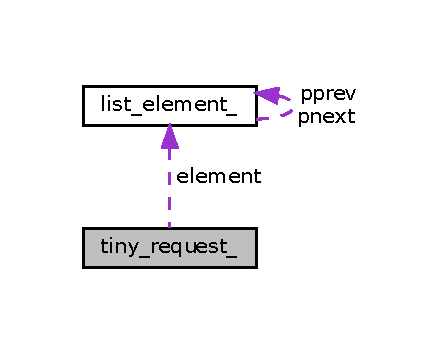
\includegraphics[width=212pt]{structtiny__request____coll__graph}
\end{center}
\end{figure}
\subsection*{Public Attributes}
\begin{DoxyCompactItemize}
\item 
\mbox{\Hypertarget{structtiny__request___a02c8fb6d26d0cfb0264423a1cb643159}\label{structtiny__request___a02c8fb6d26d0cfb0264423a1cb643159}} 
\hyperlink{structlist__element__}{list\+\_\+element} \hyperlink{structtiny__request___a02c8fb6d26d0cfb0264423a1cb643159}{element}
\begin{DoxyCompactList}\small\item\em This is base data for tiny lists. Must be first field in the structure. \end{DoxyCompactList}\item 
\mbox{\Hypertarget{structtiny__request___a019207b55569a48a82a2922dd3cc7eb2}\label{structtiny__request___a019207b55569a48a82a2922dd3cc7eb2}} 
uint8\+\_\+t \hyperlink{structtiny__request___a019207b55569a48a82a2922dd3cc7eb2}{state}
\begin{DoxyCompactList}\small\item\em state of the request \end{DoxyCompactList}\item 
\mbox{\Hypertarget{structtiny__request___aefa85d07e09d6772963532b6cf1ed125}\label{structtiny__request___aefa85d07e09d6772963532b6cf1ed125}} 
uint16\+\_\+t \hyperlink{structtiny__request___aefa85d07e09d6772963532b6cf1ed125}{uid}
\begin{DoxyCompactList}\small\item\em unique id of the sent packet \end{DoxyCompactList}\end{DoxyCompactItemize}


\subsection{Detailed Description}
defines type for tiny request list item 

The documentation for this struct was generated from the following file\+:\begin{DoxyCompactItemize}
\item 
src/proto/half\+\_\+duplex/tiny\+\_\+rq\+\_\+pool.\+h\end{DoxyCompactItemize}

\chapter{File Documentation}
\hypertarget{tiny__hd_8h}{}\section{src/proto/half\+\_\+duplex/tiny\+\_\+hd.h File Reference}
\label{tiny__hd_8h}\index{src/proto/half\+\_\+duplex/tiny\+\_\+hd.\+h@{src/proto/half\+\_\+duplex/tiny\+\_\+hd.\+h}}


Tiny Protocol Half Duplex A\+PI.  


{\ttfamily \#include $<$stdint.\+h$>$}\newline
{\ttfamily \#include \char`\"{}proto/hdlc/tiny\+\_\+hdlc.\+h\char`\"{}}\newline
{\ttfamily \#include \char`\"{}proto/hal/tiny\+\_\+types.\+h\char`\"{}}\newline
Include dependency graph for tiny\+\_\+hd.\+h\+:\nopagebreak
\begin{figure}[H]
\begin{center}
\leavevmode
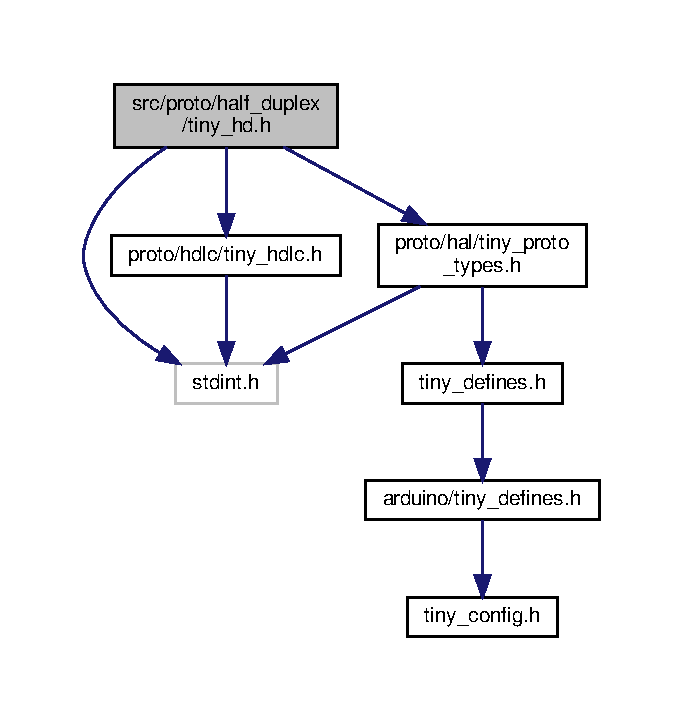
\includegraphics[width=332pt]{tiny__hd_8h__incl}
\end{center}
\end{figure}
This graph shows which files directly or indirectly include this file\+:\nopagebreak
\begin{figure}[H]
\begin{center}
\leavevmode
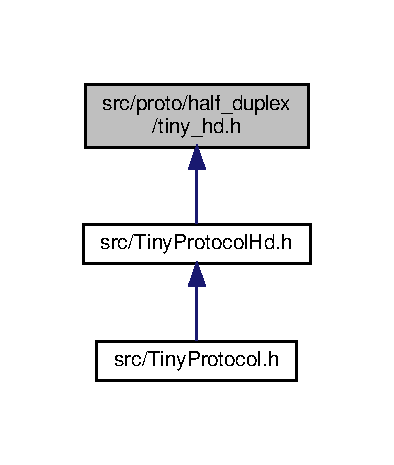
\includegraphics[width=199pt]{tiny__hd_8h__dep__incl}
\end{center}
\end{figure}
\subsection*{Classes}
\begin{DoxyCompactItemize}
\item 
struct \hyperlink{structSTinyHdData__}{S\+Tiny\+Hd\+Data\+\_\+}
\item 
struct \hyperlink{structSTinyHdInit__}{S\+Tiny\+Hd\+Init\+\_\+}
\end{DoxyCompactItemize}
\subsection*{Typedefs}
\begin{DoxyCompactItemize}
\item 
typedef struct \hyperlink{structSTinyHdData__}{S\+Tiny\+Hd\+Data\+\_\+} \hyperlink{group__HALF__DUPLEX__API_gaf9f81ad129b754a780dfca5dcd7f7cf9}{S\+Tiny\+Hd\+Data}
\item 
typedef struct \hyperlink{structSTinyHdInit__}{S\+Tiny\+Hd\+Init\+\_\+} \hyperlink{group__HALF__DUPLEX__API_ga784f1a0f0ae7f06da4bc288fa3f22408}{S\+Tiny\+Hd\+Init}
\end{DoxyCompactItemize}
\subsection*{Functions}
\begin{DoxyCompactItemize}
\item 
int \hyperlink{group__HALF__DUPLEX__API_ga747e6a3a0b5d2a9e1fe0c143c20057e9}{tiny\+\_\+hd\+\_\+init} (\hyperlink{group__HALF__DUPLEX__API_gaf9f81ad129b754a780dfca5dcd7f7cf9}{S\+Tiny\+Hd\+Data} $\ast$handle, \hyperlink{group__HALF__DUPLEX__API_ga784f1a0f0ae7f06da4bc288fa3f22408}{S\+Tiny\+Hd\+Init} $\ast$init)
\begin{DoxyCompactList}\small\item\em Initialized communication for Tiny Half Duplex protocol. \end{DoxyCompactList}\item 
void \hyperlink{group__HALF__DUPLEX__API_ga275846730a88b9654345d5defbda31e7}{tiny\+\_\+hd\+\_\+close} (\hyperlink{group__HALF__DUPLEX__API_gaf9f81ad129b754a780dfca5dcd7f7cf9}{S\+Tiny\+Hd\+Data} $\ast$handle)
\begin{DoxyCompactList}\small\item\em stops Tiny Half Duplex state machine \end{DoxyCompactList}\item 
int \hyperlink{group__HALF__DUPLEX__API_gac962595f09883dea1dd0992a608a17b9}{tiny\+\_\+hd\+\_\+run} (\hyperlink{group__HALF__DUPLEX__API_gaf9f81ad129b754a780dfca5dcd7f7cf9}{S\+Tiny\+Hd\+Data} $\ast$handle)
\begin{DoxyCompactList}\small\item\em runs receive functions of Tiny Half Duplex protocol. \end{DoxyCompactList}\item 
int \hyperlink{group__HALF__DUPLEX__API_ga84325cc961c3f31e2ba6111d0235bd61}{tiny\+\_\+hd\+\_\+run\+\_\+tx} (\hyperlink{group__HALF__DUPLEX__API_gaf9f81ad129b754a780dfca5dcd7f7cf9}{S\+Tiny\+Hd\+Data} $\ast$handle)
\item 
int \hyperlink{group__HALF__DUPLEX__API_ga5aad8dcb504b80bac923496f2686a6d6}{tiny\+\_\+send\+\_\+wait\+\_\+ack} (\hyperlink{group__HALF__DUPLEX__API_gaf9f81ad129b754a780dfca5dcd7f7cf9}{S\+Tiny\+Hd\+Data} $\ast$handle, void $\ast$buf, uint16\+\_\+t len)
\begin{DoxyCompactList}\small\item\em Sends userdata and waits for acknowledgement from remote side. \end{DoxyCompactList}\end{DoxyCompactItemize}


\subsection{Detailed Description}
Tiny Protocol Half Duplex A\+PI. 

This is Tiny Half-\/\+Duplex protocol implementation for microcontrollers. It is built on top of Tiny Protocol (tiny\+\_\+layer2.\+c) 
\hypertarget{tiny__layer2_8h}{}\section{src/proto/tiny\+\_\+layer2.h File Reference}
\label{tiny__layer2_8h}\index{src/proto/tiny\+\_\+layer2.\+h@{src/proto/tiny\+\_\+layer2.\+h}}


Tiny protocol A\+PI.  


{\ttfamily \#include $<$stdint.\+h$>$}\newline
{\ttfamily \#include \char`\"{}tiny\+\_\+proto\+\_\+types.\+h\char`\"{}}\newline
Include dependency graph for tiny\+\_\+layer2.\+h\+:
\nopagebreak
\begin{figure}[H]
\begin{center}
\leavevmode
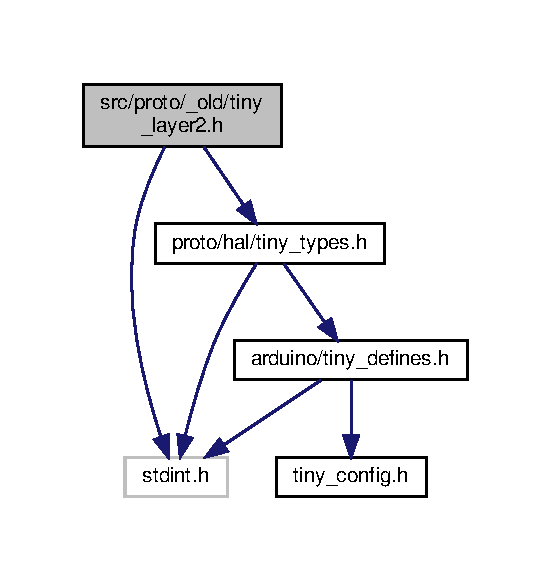
\includegraphics[width=249pt]{tiny__layer2_8h__incl}
\end{center}
\end{figure}
This graph shows which files directly or indirectly include this file\+:
\nopagebreak
\begin{figure}[H]
\begin{center}
\leavevmode
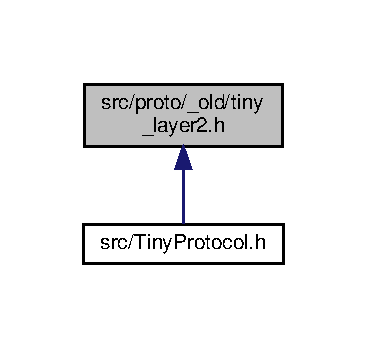
\includegraphics[width=350pt]{tiny__layer2_8h__dep__incl}
\end{center}
\end{figure}
\subsection*{Classes}
\begin{DoxyCompactItemize}
\item 
struct \hyperlink{structSTinyRxStatus}{S\+Tiny\+Rx\+Status}
\item 
struct \hyperlink{structSTinyTxStatus}{S\+Tiny\+Tx\+Status}
\item 
struct \hyperlink{structSTinyData}{S\+Tiny\+Data}
\end{DoxyCompactItemize}
\subsection*{Functions}
\begin{DoxyCompactItemize}
\item 
int \hyperlink{group__SIMPLE__API_gab9bfaed3c75551c8b7f3f8b25e766546}{tiny\+\_\+init} (\hyperlink{structSTinyData}{S\+Tiny\+Data} $\ast$handle, \hyperlink{tiny__proto__types_8h_a7f69e669de5baa69a43ee5cb439a7496}{write\+\_\+block\+\_\+cb\+\_\+t} write\+\_\+func, \hyperlink{tiny__proto__types_8h_ae3d867e030f59de94508902f2b84a7ec}{read\+\_\+block\+\_\+cb\+\_\+t} read\+\_\+func, void $\ast$pdata)
\item 
int \hyperlink{group__SIMPLE__API_ga48cf9ffab9eeb9665e61ae69e28938b8}{tiny\+\_\+close} (\hyperlink{structSTinyData}{S\+Tiny\+Data} $\ast$handle)
\item 
int \hyperlink{group__SIMPLE__API_ga988a41addbe75dc15cc13006de6740e0}{tiny\+\_\+send} (\hyperlink{structSTinyData}{S\+Tiny\+Data} $\ast$handle, uint16\+\_\+t $\ast$uid, uint8\+\_\+t $\ast$pbuf, int len, uint8\+\_\+t flags)
\begin{DoxyCompactList}\small\item\em sends frame with user payload to communication channel \end{DoxyCompactList}\item 
int \hyperlink{group__SIMPLE__API_ga470d59a60a496944e63031ba43a00e3d}{tiny\+\_\+read} (\hyperlink{structSTinyData}{S\+Tiny\+Data} $\ast$handle, uint16\+\_\+t $\ast$uid, uint8\+\_\+t $\ast$pbuf, int len, uint8\+\_\+t flags)
\item 
int \hyperlink{group__SIMPLE__API_gafae39ccf72f1f22f4dc47bd54998e88c}{tiny\+\_\+simple\+\_\+send} (\hyperlink{structSTinyData}{S\+Tiny\+Data} $\ast$handle, uint8\+\_\+t $\ast$pbuf, int len)
\begin{DoxyCompactList}\small\item\em sends frame with user payload to communication channel in blocking mode \end{DoxyCompactList}\item 
int \hyperlink{group__SIMPLE__API_gac9eaac50ab16b9891ca74e5c5e46b778}{tiny\+\_\+simple\+\_\+read} (\hyperlink{structSTinyData}{S\+Tiny\+Data} $\ast$handle, uint8\+\_\+t $\ast$pbuf, int len)
\begin{DoxyCompactList}\small\item\em reads frame from the channel in blocking mode. \end{DoxyCompactList}\item 
void \hyperlink{group__ADVANCED__API_gac5cabf56a5b22e96036b9e5bff926f1d}{tiny\+\_\+enable\+\_\+uid} (\hyperlink{structSTinyData}{S\+Tiny\+Data} $\ast$handle, uint8\+\_\+t on)
\begin{DoxyCompactList}\small\item\em The function enables uid support. Enables uid support. The function affects on tiny\+\_\+on\+\_\+rx\+\_\+byte and on\+\_\+frame\+\_\+cb\+\_\+t behavior. \end{DoxyCompactList}\item 
int \hyperlink{group__ADVANCED__API_ga5e66725a2818491d4e2b1134951d9229}{tiny\+\_\+set\+\_\+fcs\+\_\+bits} (\hyperlink{structSTinyData}{S\+Tiny\+Data} $\ast$handle, uint8\+\_\+t bits)
\item 
int \hyperlink{group__ADVANCED__API_gaaf9bf6423bd0b8388c3387225b805278}{tiny\+\_\+on\+\_\+rx\+\_\+byte} (\hyperlink{structSTinyData}{S\+Tiny\+Data} $\ast$handle, uint8\+\_\+t $\ast$pbuf, int len, uint8\+\_\+t byte)
\begin{DoxyCompactList}\small\item\em The function processes one rx byte. Used in event-\/based mode. This function processes single received byte. If new frame is completely received, read\+\_\+cb handler is called and application can take actions on receive frame. Refer to tiny\+\_\+set\+\_\+callbacks. \end{DoxyCompactList}\item 
int \hyperlink{group__ADVANCED__API_ga159189fa29f3eaa79a76a3fa87b31084}{tiny\+\_\+send\+\_\+start} (\hyperlink{structSTinyData}{S\+Tiny\+Data} $\ast$handle, uint8\+\_\+t flags)
\begin{DoxyCompactList}\small\item\em initiates sending of a new frame \end{DoxyCompactList}\item 
int \hyperlink{group__ADVANCED__API_gabe04a4e76adc5421deac4e3699a15646}{tiny\+\_\+send\+\_\+buffer} (\hyperlink{structSTinyData}{S\+Tiny\+Data} $\ast$handle, uint8\+\_\+t $\ast$pbuf, int len, uint8\+\_\+t flags)
\begin{DoxyCompactList}\small\item\em sends user provided data in the body of the frame \end{DoxyCompactList}\item 
int \hyperlink{group__ADVANCED__API_ga2e85c7e9efb0bbe9c6adfd923ec7c73c}{tiny\+\_\+send\+\_\+end} (\hyperlink{structSTinyData}{S\+Tiny\+Data} $\ast$handle, uint8\+\_\+t flags)
\begin{DoxyCompactList}\small\item\em completes sending of a new frame \end{DoxyCompactList}\item 
void \hyperlink{group__ADVANCED__API_ga73c9f1cfb0948bd559d3704749db540b}{tiny\+\_\+send\+\_\+terminate} (\hyperlink{structSTinyData}{S\+Tiny\+Data} $\ast$handle)
\begin{DoxyCompactList}\small\item\em terminates send operation \end{DoxyCompactList}\item 
int \hyperlink{group__ADVANCED__API_ga2f0547115de5b96a828d79f5491d22fa}{tiny\+\_\+read\+\_\+start} (\hyperlink{structSTinyData}{S\+Tiny\+Data} $\ast$handle, uint8\+\_\+t flags)
\begin{DoxyCompactList}\small\item\em initiates receiving of a new frame \end{DoxyCompactList}\item 
int \hyperlink{group__ADVANCED__API_gade4e07eb12b8e32e6dd0c7b9757e8f39}{tiny\+\_\+read\+\_\+buffer} (\hyperlink{structSTinyData}{S\+Tiny\+Data} $\ast$handle, uint8\+\_\+t $\ast$pbuf, int len, uint8\+\_\+t flags)
\begin{DoxyCompactList}\small\item\em reads frame payload to provided buffer \end{DoxyCompactList}\item 
void \hyperlink{group__ADVANCED__API_gaab48caab81a46d74fb52f2afb2649b61}{tiny\+\_\+read\+\_\+terminate} (\hyperlink{structSTinyData}{S\+Tiny\+Data} $\ast$handle)
\begin{DoxyCompactList}\small\item\em terminates read operation \end{DoxyCompactList}\item 
int \hyperlink{group__ADVANCED__API_gac318682c20279f9f20ffc6f636a7f1c9}{tiny\+\_\+lock} (\hyperlink{structSTinyData}{S\+Tiny\+Data} $\ast$handle, uint8\+\_\+t flags)
\begin{DoxyCompactList}\small\item\em locks Tiny state machine for send operations \end{DoxyCompactList}\item 
void \hyperlink{group__ADVANCED__API_gae4bfad55a4ef5814a5af50f044f6d7cd}{tiny\+\_\+unlock} (\hyperlink{structSTinyData}{S\+Tiny\+Data} $\ast$handle)
\begin{DoxyCompactList}\small\item\em unlock Tiny state machine for send operations \end{DoxyCompactList}\item 
int \hyperlink{group__ADVANCED__API_gac562103dd1699b82fddf29dccdc0ec7c}{tiny\+\_\+set\+\_\+callbacks} (\hyperlink{structSTinyData}{S\+Tiny\+Data} $\ast$handle, \hyperlink{tiny__proto__types_8h_ad6bf709565b8aecb9e6ecf196f219d54}{on\+\_\+frame\+\_\+cb\+\_\+t} read\+\_\+cb, \hyperlink{tiny__proto__types_8h_ad6bf709565b8aecb9e6ecf196f219d54}{on\+\_\+frame\+\_\+cb\+\_\+t} send\+\_\+cb)
\begin{DoxyCompactList}\small\item\em set callbacks for processing frames The function sets callback procs for specified Tiny channel. callbacks will receive all data being sent or received. \end{DoxyCompactList}\item 
int \hyperlink{group__ADVANCED__API_gabe38a1f81966f6901eb2f6969b568298}{tiny\+\_\+get\+\_\+callbacks} (\hyperlink{structSTinyData}{S\+Tiny\+Data} $\ast$handle, \hyperlink{tiny__proto__types_8h_ad6bf709565b8aecb9e6ecf196f219d54}{on\+\_\+frame\+\_\+cb\+\_\+t} $\ast$read\+\_\+cb, \hyperlink{tiny__proto__types_8h_ad6bf709565b8aecb9e6ecf196f219d54}{on\+\_\+frame\+\_\+cb\+\_\+t} $\ast$send\+\_\+cb)
\begin{DoxyCompactList}\small\item\em returns callbacks assigned for frame processing The function returns set callbacks. \end{DoxyCompactList}\item 
int \hyperlink{group__ADVANCED__API_ga5f61774b2027a91f772f31d943acdd3f}{tiny\+\_\+get\+\_\+stat} (\hyperlink{structSTinyData}{S\+Tiny\+Data} $\ast$handle, \hyperlink{structSTinyStats}{S\+Tiny\+Stats} $\ast$stat)
\item 
int \hyperlink{group__ADVANCED__API_gac75ee03ea3691b0a8bf842d764b342d9}{tiny\+\_\+clear\+\_\+stat} (\hyperlink{structSTinyData}{S\+Tiny\+Data} $\ast$handle)
\end{DoxyCompactItemize}


\subsection{Detailed Description}
Tiny protocol A\+PI. 

This is Tiny protocol implementation for microcontrollers 
\hypertarget{arduino_8dox}{}\section{src/arduino.dox File Reference}
\label{arduino_8dox}\index{src/arduino.\+dox@{src/arduino.\+dox}}


Arduino reated A\+PI.  




\subsection{Detailed Description}
Arduino reated A\+PI. 


\hypertarget{TinyLightProtocol_8h}{}\section{src/\+Tiny\+Light\+Protocol.h File Reference}
\label{TinyLightProtocol_8h}\index{src/\+Tiny\+Light\+Protocol.\+h@{src/\+Tiny\+Light\+Protocol.\+h}}


Tiny light protocol Arduino A\+PI.  


{\ttfamily \#include \char`\"{}Tiny\+Packet.\+h\char`\"{}}\newline
{\ttfamily \#include \char`\"{}proto/tiny\+\_\+light.\+h\char`\"{}}\newline
{\ttfamily \#include $<$Hardware\+Serial.\+h$>$}\newline
Include dependency graph for Tiny\+Light\+Protocol.\+h\+:
\nopagebreak
\begin{figure}[H]
\begin{center}
\leavevmode
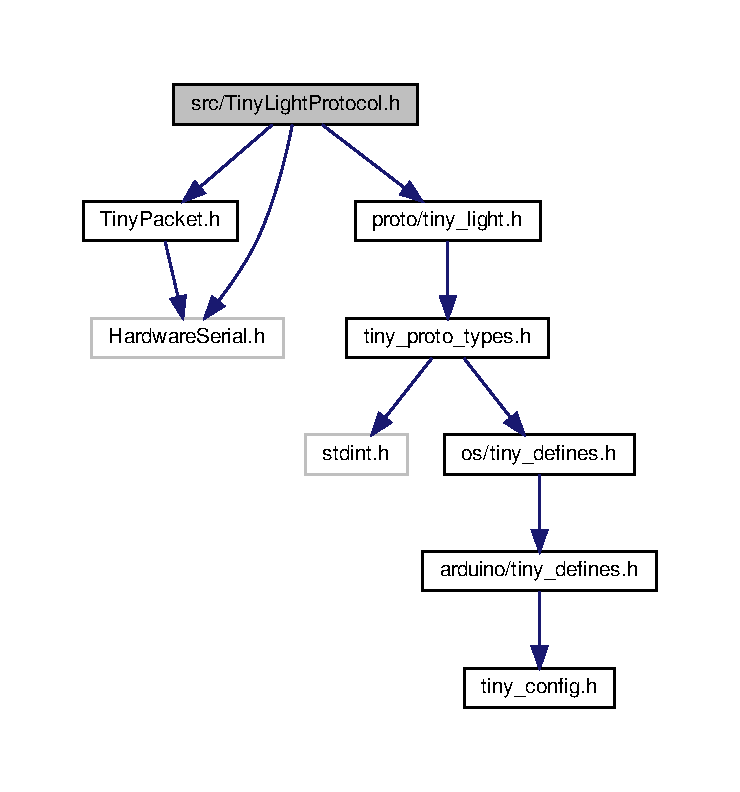
\includegraphics[width=350pt]{TinyLightProtocol_8h__incl}
\end{center}
\end{figure}
\subsection*{Classes}
\begin{DoxyCompactItemize}
\item 
class \hyperlink{classTiny_1_1ProtoLight}{Tiny\+::\+Proto\+Light}
\end{DoxyCompactItemize}


\subsection{Detailed Description}
Tiny light protocol Arduino A\+PI. 

This is Tiny light protocol implementation for microcontrollers 
\hypertarget{TinyPacket_8h}{}\section{src/\+Tiny\+Packet.h File Reference}
\label{TinyPacket_8h}\index{src/\+Tiny\+Packet.\+h@{src/\+Tiny\+Packet.\+h}}


Tiny protocol Arduino A\+PI.  


{\ttfamily \#include $<$Hardware\+Serial.\+h$>$}\newline
Include dependency graph for Tiny\+Packet.\+h\+:\nopagebreak
\begin{figure}[H]
\begin{center}
\leavevmode
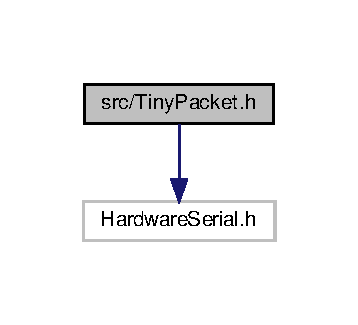
\includegraphics[width=172pt]{TinyPacket_8h__incl}
\end{center}
\end{figure}
This graph shows which files directly or indirectly include this file\+:\nopagebreak
\begin{figure}[H]
\begin{center}
\leavevmode
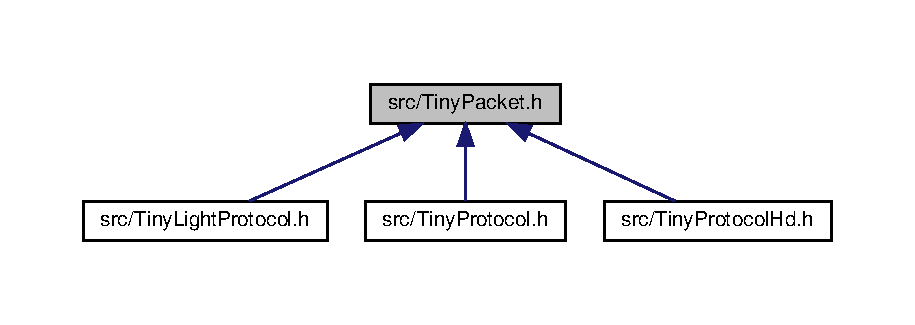
\includegraphics[width=350pt]{TinyPacket_8h__dep__incl}
\end{center}
\end{figure}
\subsection*{Classes}
\begin{DoxyCompactItemize}
\item 
class \hyperlink{classTiny_1_1Packet}{Tiny\+::\+Packet}
\end{DoxyCompactItemize}


\subsection{Detailed Description}
Tiny protocol Arduino A\+PI. 

This is Tiny protocol implementation for microcontrollers 
\hypertarget{TinyProtocol_8h}{}\section{src/arduino/src/\+Tiny\+Protocol.h File Reference}
\label{TinyProtocol_8h}\index{src/arduino/src/\+Tiny\+Protocol.\+h@{src/arduino/src/\+Tiny\+Protocol.\+h}}


Tiny protocol Arduino A\+P\+I.  


{\ttfamily \#include \char`\"{}proto/tiny\+\_\+layer2.\+h\char`\"{}}\\*
{\ttfamily \#include $<$Hardware\+Serial.\+h$>$}\\*
Include dependency graph for Tiny\+Protocol.\+h\+:
\nopagebreak
\begin{figure}[H]
\begin{center}
\leavevmode
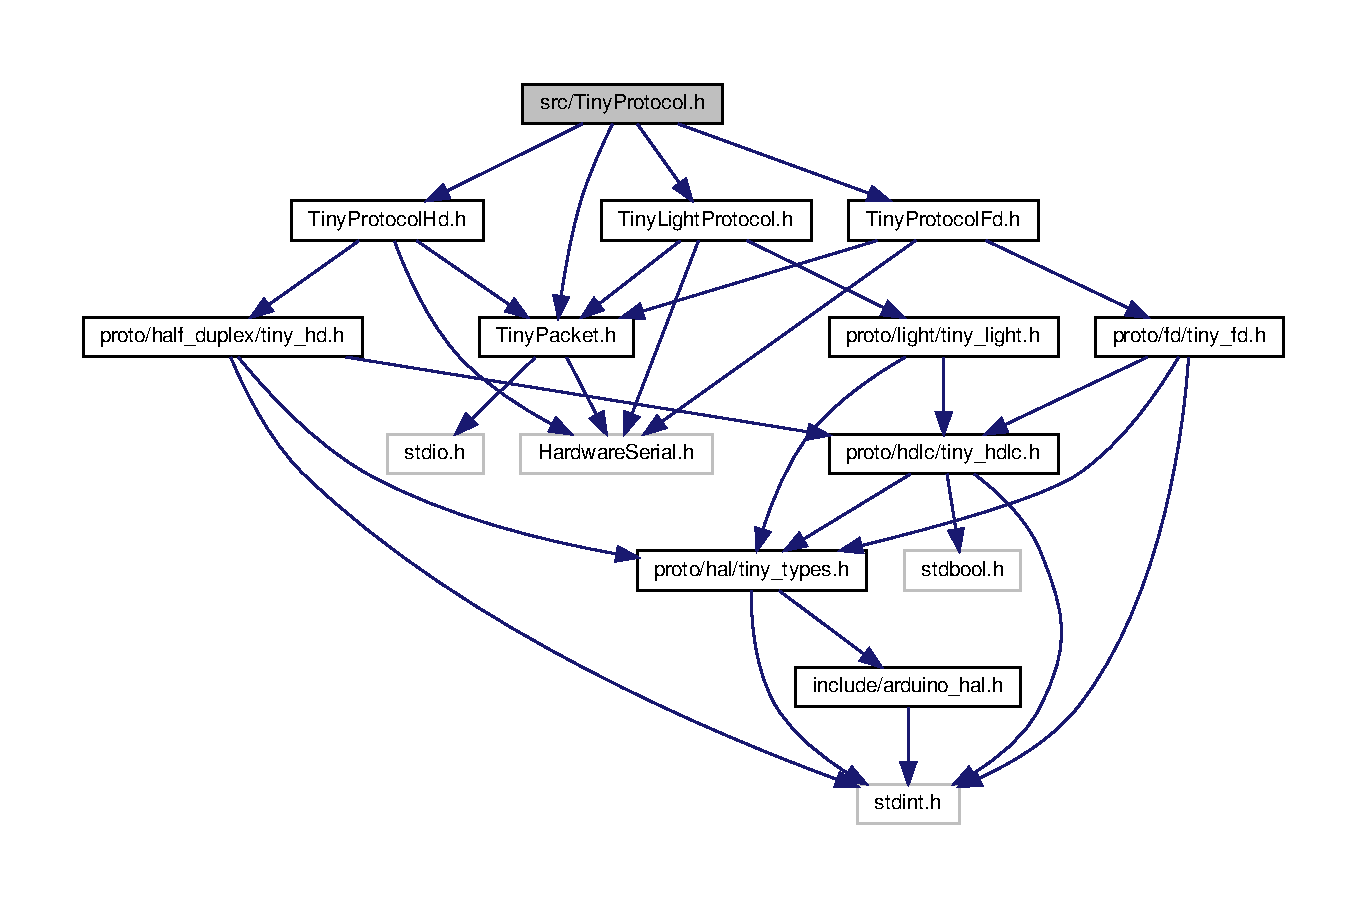
\includegraphics[width=350pt]{TinyProtocol_8h__incl}
\end{center}
\end{figure}
\subsection*{Classes}
\begin{DoxyCompactItemize}
\item 
class \hyperlink{classTiny_1_1Proto}{Tiny\+::\+Proto}
\item 
class \hyperlink{classTiny_1_1Packet}{Tiny\+::\+Packet}
\end{DoxyCompactItemize}


\subsection{Detailed Description}
Tiny protocol Arduino A\+P\+I. 

This is Tiny protocol implementation for microcontrollers 
\hypertarget{TinyProtocolHd_8h}{}\section{src/arduino/src/\+Tiny\+Protocol\+Hd.h File Reference}
\label{TinyProtocolHd_8h}\index{src/arduino/src/\+Tiny\+Protocol\+Hd.\+h@{src/arduino/src/\+Tiny\+Protocol\+Hd.\+h}}


Tiny protocol Arduino A\+P\+I.  


{\ttfamily \#include \char`\"{}Tiny\+Packet.\+h\char`\"{}}\\*
{\ttfamily \#include \char`\"{}proto/tiny\+\_\+hd.\+h\char`\"{}}\\*
{\ttfamily \#include $<$Hardware\+Serial.\+h$>$}\\*
Include dependency graph for Tiny\+Protocol\+Hd.\+h\+:
\nopagebreak
\begin{figure}[H]
\begin{center}
\leavevmode
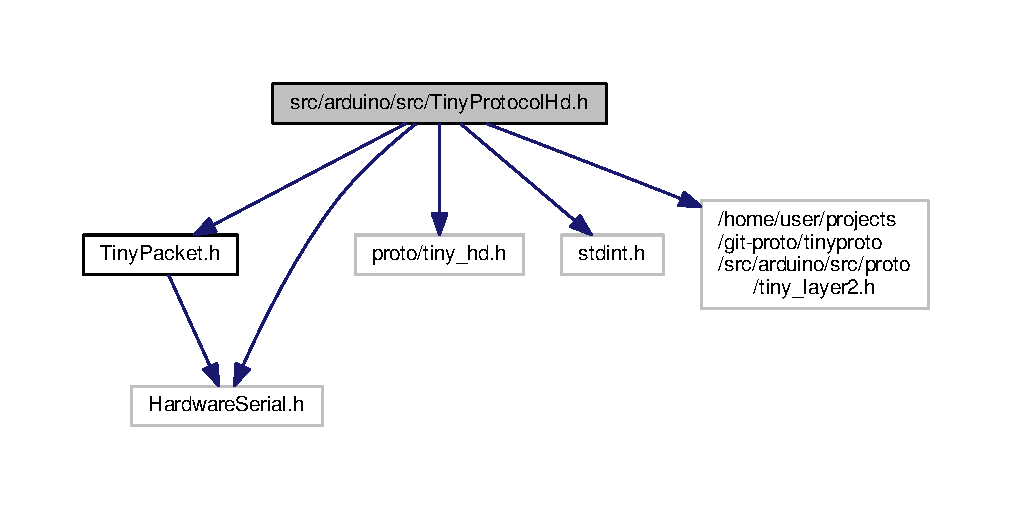
\includegraphics[width=350pt]{TinyProtocolHd_8h__incl}
\end{center}
\end{figure}
\subsection*{Classes}
\begin{DoxyCompactItemize}
\item 
class \hyperlink{classTiny_1_1ProtoHd}{Tiny\+::\+Proto\+Hd}
\end{DoxyCompactItemize}


\subsection{Detailed Description}
Tiny protocol Arduino A\+P\+I. 

This is Tiny protocol implementation for microcontrollers 
\hypertarget{mainpage_8dox}{}\section{src/mainpage.dox File Reference}
\label{mainpage_8dox}\index{src/mainpage.\+dox@{src/mainpage.\+dox}}


Tiny Microcontroller Communication Protocol.  




\subsection{Detailed Description}
Tiny Microcontroller Communication Protocol. 


%--- End generated contents ---

% Index
\backmatter
\newpage
\phantomsection
\clearemptydoublepage
\addcontentsline{toc}{chapter}{Index}
\printindex

\end{document}
